% =====================================================================
%  TETC-2026-05-0252 -- BAN CO DANH DAU THAY DOI
%
%  Giong het ban sach (main_revision.tex), chi khac: bat co \annottrue nen
%  moi tieu de muc hien them mot nhan mau noi muc do MOI / VIET LAI / SUA
%  LOI / GIU, kem mot cau giai thich va ma y reviewer tuong ung.
%
%  Dung de:
%    1. Thay va dong tac gia doc soat -- nhin la biet cho nao moi, cho nao
%       con nguyen cua ban da nop, khong phai do hai ban canh nhau.
%    2. TETC bat buoc nop ban danh dau thay doi cung voi ban sach.
%
%  Noi dung than bai KHONG khac ban sach mot chu nao -- ca hai deu
%  % =====================================================================
%  THAN TAI LIEU dung chung: tieu de, tac gia, abstract, va thu tu cac muc.
%  Khong chua lenh mo tai lieu -- hai ban main bao ngoai phan nay.
% =====================================================================
\title{NISQ-Aware Quantum Kernel SVM for Network\\
  Intrusion Detection:\\
  A Regime-Specific Benchmark on NSL-KDD}

\author{Minh~Tuan~Pham,
        Phuc~Hao~Do,
        Nguyen~Nang~Hung~Van,
        Quang~Anh~Nguyen,
        and~Quan~Tran~Anh~Vo% <-- GIU NGUYEN, khong them/bot tac gia
\thanks{Manuscript received [Date]; revised [Date]. This work was supported by
The University of Danang - University of Science and Technology under Project
T2026-02-10TN. \emph{(Corresponding author: Quan Tran Anh Vo.)}}
\thanks{Phuc Hao Do is with The Bonch-Bruevich Saint Petersburg State University
of Telecommunications, Saint Petersburg 193232, Russia, and also with Danang
Architecture University, Danang 550000, Vietnam (e-mail: do.hf@sut.ru;
haodp@dau.edu.vn).}
\thanks{Minh Tuan Pham, Nguyen Nang Hung Van, Quang Anh Nguyen, and Quan Tran
Anh Vo are with the University of Science and Technology - The University of
Danang, Danang 550000, Vietnam (e-mail: pmtuan@dut.udn.vn;
nguyenvan@dut.udn.vn; anh1303052005@gmail.com; votrananhquan1111@gmail.com).}}

\markboth{IEEE Transactions on Emerging Topics in Computing,~Vol.~XX, No.~Y, 2026}%
{Pham \MakeLowercase{\textit{et al.}}: NISQ-Aware Quantum Kernel SVM for Network Intrusion Detection}

\maketitle

% =====================================================================
%  ABSTRACT -- viet lai. Ban da nop khang dinh loi the o che do it du lieu
%  va o dich chuyen prior; ca hai deu khong con dung sau khi them baseline
%  manh va do lai voi 10 run. Abstract moi dan bang cau hoi "o dau" chu
%  khong bang mot con so thang cuoc.
% =====================================================================
\begin{abstract}
\begin{revbody}
Quantum support vector machines (QSVM) built on the \ZZ{}-feature map are
routinely reported to help on network intrusion detection (NIDS), yet the
conditions under which they help are rarely isolated. This paper asks where a
NISQ-feasible quantum kernel is worth its cost, where ``NISQ-aware'' means a
circuit budget (four qubits, depth two, 44 two-qubit gates) chosen under an
explicit cost model and checked under a backend-derived noise model in
simulation, not execution on hardware, and answers with a protocol in
which one factor is varied at a time: the embedding dimension is fixed by a
lexicographic rule that charges explicitly for two-qubit gate count; the
entangling layer is ablated against an otherwise identical control; the test
distribution is shifted; and the training-set size is swept across two orders of
magnitude under both the natural class prior and a rare-enriched one. Every
comparison is paired within run over ten runs, tuned symmetrically for quantum
and classical models alike, and corrected for multiplicity within baseline
families; under a single Benjamini--Hochberg correction over all cells the
tally below becomes 17, 15 and 78, and under Holm over all 110 cells no
verdict survives. Against six baselines that now include a
random forest and XGBoost, we find no general advantage: of 110 controlled
comparisons, 21 favour the quantum kernel, 21 favour a classical baseline, and
68 are inconclusive, and the cells come from two protocols (a rare-enriched
pool with small test splits, and the natural prior on the full test set) that
are tallied separately in the paper. What we do find is structure. Under the
natural class prior the ordering against the two tree ensembles and the linear
and polynomial kernels reverses between $N=2000$ and $N=5000$ and survives
freezing the hyper-parameters; against the RBF kernel it does not demonstrably
reverse at any size tested, and against XGBoost given all 122 features the
kernel reaches parity, not a lead. Whether rare-attack enrichment, as the
submitted protocol used, removes the reversal cannot be decided by this design:
the enriched arm cannot be run past $N=2000$ without runs sharing samples, and
where the two arms overlap the tree ensembles lead under both priors. The selection rule transfers to
UNSW-NB15 unchanged and returns six qubits rather than four, while the
sample-complexity reversal does not transfer. Finally, spending a larger feature
budget forces a wider circuit, and widening destroys the kernel: at eight qubits
all 48 paired comparisons favour the classical model, with a mechanism visible
directly in the Gram matrix, whose off-diagonal dispersion decays faster for the
\ZZ{} map than for its entanglement-free control, by the factor of two that
phase-term counting predicts at $K=20$ and by 3.3 at $K=80$, where the collapse
occurs. We report the result as a regime map, including the regimes in which the
quantum kernel loses.
\end{revbody}
\end{abstract}

\begin{IEEEkeywords}
Quantum machine learning, quantum kernel, support vector machine, network
intrusion detection, NSL-KDD, UNSW-NB15, NISQ, \ZZ{}FeatureMap, kernel
concentration, sample complexity, class-prior shift.
\end{IEEEkeywords}

% =====================================================================
\section{Introduction}
\label{sec:intro}
% =====================================================================
%  I. Introduction
%
%  Ban da nop mo bai bang "QSVM dat 0.854, hon SVM-RBF 0.838". So do gio
%  khong con dung (XGBoost 0.8503 dung dau). Ban nay mo bang CAU HOI, va
%  noi thang ngay o trang 1 rang phan lon ket qua la am hoac khong ket luan
%  duoc. Reviewer doc trang 1 phai thay ngay minh khong ban loi the.
%
%  Dong cuoi cua danh sach dong gop la cho tu khai 5 khang dinh phai rut.
%  De o day chu khong giau xuong muc VII: neu reviewer tu tim ra thi mat
%  het thien chi.
% =====================================================================

\revnote{rewrite}{Rewritten. The submitted introduction claimed a low-data and prior-shift advantage; both are withdrawn (AE-1, R1-4).}
\begin{revbody}
Network intrusion detection is an attractive target for quantum machine
learning. The data are tabular and moderate-dimensional, the decision is a
classification, and the operational value of a small accuracy gain is high
\cite{ref24}. Classical machine learning and deep learning are well established
on the task \cite{ref1,ref2,ref3}, which sets the bar a quantum method has to
clear. Quantum kernel methods are the natural instrument: a feature map prepares a
state whose fidelities form a positive semi-definite kernel that can be dropped
into a standard support vector machine \cite{havlicek2019,schuld2019}, so the
quantum component is a single well-isolated block inside an otherwise classical
pipeline.

The literature reflects that attractiveness. Studies applying quantum kernels
and variational classifiers to NSL-KDD \cite{ref4} and its successors
\cite{ref25} report accuracies competitive with, and sometimes above,
classical baselines \cite{ref13,ref14,ref15}. What they rarely report is the shape of the claim: at which training
set size, against which class prior, at which circuit width, and against which
classical opponent. Those choices are not incidental. We show below that varying
only the training-set size, with everything else fixed, is enough to reverse the
ordering between a quantum kernel and the tree ensembles and the linear and
polynomial kernels we tested, on a shared four-dimensional embedding.
A benchmark conducted at one operating point can therefore report an advantage
or a deficit and be internally consistent in either case.

This paper asks a narrower question than the literature usually asks:
\emph{where} is a NISQ-feasible quantum kernel worth its cost? The question is
posed as a regime-identification problem (Problem~\ref{prob:regime}) whose
answers include the regimes where the answer is ``nowhere we can detect''.

Our protocol varies one factor at a time. The embedding dimension is fixed by a
lexicographic rule that charges explicitly for two-qubit gates, before any
downstream metric is inspected. The entangling layer is ablated against an
otherwise identical control. The test distribution is shifted four ways. The
training-set size is swept over two orders of magnitude under both the natural
class prior and a rare-enriched one. Every comparison is paired within run over
ten runs, both quantum and classical models are tuned by the same procedure on
the same held-out set, and $p$-values are Holm-corrected within baseline
families. The baselines include a random forest and XGBoost, which the submitted
version of this work did not.

The headline is a map, not a number. Of $110$ controlled comparisons, $21$
favour the quantum kernel, $21$ favour a classical baseline, and $68$ are
inconclusive. Inside that map there is structure worth reporting:

\begin{itemize}
  \item \textbf{An ordering that reverses with sample size.} Under the natural
    class prior, on the shared four-component embedding, \QSVM{} is the
    second-worst model at $N=100$ and the best at $N=10^{4}$; the paired
    difference against XGBoost and the random forest changes sign between
    $N=2000$ and $N=5000$ in both tuning arms and reaches corrected
    significance, the sign change against SVM-RBF is $+0.0008$ and never
    significant, and against XGBoost given all $122$ features the kernel
    reaches parity rather than a lead. Whether rare-attack enrichment (the
    sampling our own submitted protocol used) removes the reversal is not
    decidable with this design: the enriched arm ends at $N=2000$, before the
    reversal, and where the two arms overlap the tree ensembles lead under
    both priors.
  \item \textbf{A selection rule that transfers.} The three-stage rule returns
    $n^{\ast}=4$ on NSL-KDD and, applied without changing a threshold,
    $n^{\ast}=6$ on UNSW-NB15, recovered on $10/10$ independent subsets. The
    entanglement ablation transfers as well; the sample-size reversal does not.
  \item \textbf{A measured boundary.} Spending a larger feature budget forces a
    wider circuit, and widening destroys the kernel: at $K=80$, where the rule
    returns $n^{\ast}=8$, all $48$ paired comparisons favour the classical
    model and the entanglement ablation reverses sign. The mechanism is visible
    in the Gram matrix, whose off-diagonal dispersion decays faster for the
    \ZZ{} map than for its entanglement-free control: by a factor of $2.02$ at
    $K=20$, the ratio the $\binom{n}{2}$ versus $n$ phase-term counting
    predicts, and by $3.32$ at $K=80$, where the collapse occurs and the
    counting argument predicts the ordering but not the rate. Across widths the
    dispersion correlates with macro-$F_{1}$ at $r=+0.77$ for the \ZZ{} map
    (seven widths, 95\% CI $[+0.04,+0.96]$); the contrast with the \Zmap{}
    map ($r=+0.32$) is not resolvable at seven points.
\end{itemize}

We also report where the method loses. It degrades faster than either tree
ensemble under class-prior shift; it is the least robust of all seven models to
feature perturbation; and although it detects rare attacks far better than the
tree ensembles, an RBF-kernel SVM detects them better still.
\end{revbody}

\subsection*{Relation to the submitted version}
\revnote{new}{New subsection: the five claims of the submitted version that are withdrawn, stated on page 1.}
\begin{revbody}

This paper is a substantially revised version of an earlier submission, and five
of that version's claims do not survive the revised protocol. We state them
here rather than in a footnote. (i)~The claimed advantage in the low-data regime
is reversed in direction. (ii)~A reported rare-attack gain of $6.7$ points with
$d=+0.68$ is withdrawn: no rare-class metric was computed by the code that
produced it. (iii)~The former Theorem~1 was false, as one reviewer identified;
it and the objective it maximised have been removed rather than repaired.
(iv)~The former Pareto stage filtered no candidate on this data and has been
replaced. (v)~With a tree ensemble in the comparison, \QSVM{} is no longer the
top-ranked model at the main operating point. Sec.~\ref{sec:erratum} gives the
technical detail, including one error no reviewer raised.
\end{revbody}


% =====================================================================
\section{Background and Related Work}
\label{sec:related}
% =====================================================================
%  II. Background and Related Work
%
%  Ba viec muc nay phai lam, theo dung thu tu uu tien cua reviewer:
%    R1-1  : them QMI 2026 (bai R1 chi dich danh) + cap nhat Table I
%    R3-5  : dinh vi ro so voi arXiv:2403.07059 va 2409.04406
%    tu giac: trich Gillani et al. (2608.18155) -- bai dong thoi, trung
%             ca hai dataset. Nop sau ho 2 thang ma lo di la reviewer tu tim ra.
%
%  Giong van: KHONG cai nhau voi R3. Neu ho noi benchmark khong phai dong
%  gop, ta neu su that la hai bai chinh ho tin cay cung la benchmark thuan
%  tuy -- roi di tiep.
% =====================================================================

\subsection{Quantum kernels}
\revnote{rewrite}{Submitted version had Definitions 1--2 and Propositions 1--2; merged, and Proposition 1 demoted to a cited fact (F1) as R3-3 asks.}
\begin{revbody}

A quantum kernel embeds $\bm{x}$ into a state $|\phi(\bm{x})\rangle$ prepared by
a parameterised circuit and reads off the fidelity as a similarity
\cite{havlicek2019,schuld2019}. The construction sits inside a broader quantum
machine learning programme \cite{ref5,ref6,ref7}, and the identification of
parameterised-circuit models with kernel machines \cite{ref9} is what makes the
quantum component substitutable into a classical learner. Separations have been
proved for constructed problems \cite{ref18}, but the conditions under which they
extend to data that arise in practice are restrictive \cite{ref19,ref20}.
Two results bound expectations. Alignment-based
bounds \cite{cristianini2002,cortes2012} say that a kernel better aligned with
the labels admits a tighter generalisation guarantee at equal empirical risk,
but say nothing about whether a given circuit produces such a kernel. In the
other direction, fidelity kernels from expressive maps concentrate exponentially
toward a constant as the qubit count grows \cite{thanasilp2024}, an effect
distinct from, though related to, the barren plateaus of variational training
\cite{ref10}, so the same expressivity \cite{ref21} that makes a map interesting
makes its Gram matrix uninformative at width. Sec.~\ref{sec:res-width} measures both effects here: the alignment gain
is large, and the concentration is what eventually destroys it.
\end{revbody}

\subsection{Quantum machine learning for intrusion detection}
\revnote{rewrite}{Adds the 2026 survey and Cirillo et al. (QMI 2026), the study Reviewer 1 named in R1-1.}
\begin{revbody}

Applications of quantum kernels and variational classifiers to network intrusion
detection have grown quickly \cite{ref13,ref14,ref15}, most using NSL-KDD
\cite{ref4} or a successor corpus \cite{ref25}; a 2026 survey \cite{kaissar2026} covers the field through
January of that year and reaches two conclusions that bear directly on this
paper: most published approaches rely on simulated quantum environments and
legacy datasets, and evaluation practice is inconsistent across studies. The
recurring pattern is a single operating point (one qubit count, one
training-set size, one class prior) with an accuracy compared against a small
set of classical baselines.

The most directly comparable study is the benchmark of Cirillo \emph{et al.}
\cite{qmi2026}, which evaluates Pegasos-QSVC, a variational classifier and a
hybrid quantum--classical network on ToN\_IoT and NSL-KDD under ideal and three
backend-derived noise models, and reports Pegasos-QSVC best at $94.60\%$
accuracy and $94.13\%$ $F_1$ on NSL-KDD.

Two of their findings bear on ours. They compare against SVM, XGBoost, random
forest and a neural network at matched dimensionality and conclude that the
classical models retain higher peak accuracy, XGBoost reaching $99.1\%$ on
ToN\_IoT, while the quantum models stay competitive in low-dimensional
feature spaces; our own ranking agrees (Sec.~\ref{sec:res-c2}). And they sweep
the qubit count from $2$ to $10$ against two-qubit gate count, finding
performance concentrated in a $20$--$35$ CNOT band and degrading beyond about
$60$. Our operating point of $24$ CNOTs sits inside that band, and the collapse
we report at $112$ is consistent with their threshold.

The two studies diverge on the mechanism, and that divergence is part of our
contribution: they attribute the degradation to two-qubit gate error
accumulating on noisy backends, whereas we observe the same collapse under
\emph{exact, noiseless} simulation and trace it to concentration of the Gram
matrix. Hardware noise is not a necessary ingredient; the bound is intrinsic to
the kernel.

What that study does not vary is the training-set size, fixed at a single $15\%$
class-balanced subsample ($15{,}114$ training instances for NSL-KDD) drawn under
a random $80/20$ split rather than the official partitions.
\end{revbody}

\subsection{Benchmarking studies of quantum models}
\revnote{new}{New subsection. The two benchmarking studies Reviewer 3 cited as prior evidence (R3-5), read in full.}
\begin{revbody}

Two broad benchmarks are relevant precisely because they are sceptical. Bowles,
Ahmed and Schuld \cite{bowles2024} evaluate twelve QML models over $160$ datasets
(predominantly synthetic, so that data properties can be controlled) in
noise-free statevector simulation at up to $18$ qubits, against an MLP, an
RBF-kernel SVM and a CNN, and find that quantum models rarely beat well-tuned
classical baselines. Schnabel and Roth \cite{schnabel2024} run over $20{,}000$
tuned models comparing fidelity and projected quantum kernels across five
dataset families, at up to $15$ qubits against RBF-kernel baselines, and use
correlation analysis to identify which design choices matter. Both conclude that
general-purpose feature maps seldom win once the classical comparison is done
properly, and our results agree with them at the aggregate level.

Neither varies the training-set size: Bowles \emph{et al.} subsample fixed
counts per task, and Schnabel and Roth fix $M=240$ training and $M'=60$ test
points throughout.

Concurrently with this revision, Gillani \emph{et al.} \cite{gillani2026}
benchmark quantum and classical models for intrusion detection across four
corpora, including both of ours, at eight qubits with a $4/6/8/12$-qubit
ablation, against five tuned classical baselines including a random forest and
XGBoost, with Benjamini--Hochberg control over $108$ comparisons on NSL-KDD.
Their conclusion, that reported quantum gains are largely attributable to the
classical preprocessing front-end once the same front-end is given to classical
models, stands in a relation to Sec.~\ref{sec:res-c4} that is closer to a
discrepancy than to corroboration, and we report it as such. Our positive
result is obtained under exactly the matched front-end they describe: every
classical baseline consumes the same four components as the circuit, and the
kernel still leads the tree ensembles at $N\geq5000$. Two differences may
account for it, and the data cannot separate them. Their comparison is made at
one training-set size, the full $125{,}973$-record partition, where our
reference arm shows full-feature XGBoost at $0.804$ above any four-qubit model;
ours sweeps $N$ and finds the lead only between $5000$ and $10^{4}$ records, on
an embedding of four dimensions. And their front-end is given to classical
models at eight qubits' worth of features, where Sec.~\ref{sec:res-width}
shows our kernel has already collapsed. Read together, the two studies agree
that the front-end carries most of what is reported as quantum advantage, and
disagree on whether a residual lead exists in a narrow window of training-set
size and embedding width that their design does not visit. We do not claim
breadth over that study: they evaluate four datasets to our two, at eight
qubits to our four and six, with a stricter error-rate criterion.
\end{revbody}

\subsection{Bounded advantage windows in adjacent domains}
\revnote{new}{New subsection. Carducci, ICAD 2026, the study Reviewer 4 named in R4-1.}
\begin{revbody}

The question this paper asks is being asked elsewhere, and in at least one
adjacent domain it has been given the same shape. Carducci \cite{carducci2026}
opens by arguing that malware analysts ``do not need another general claim that
quantum computing is either broadly superior or broadly impractical'' but rather
``need to know which kinds of malware representations justify quantum effort''
which is, on a different task, the reframing this revision makes.

That study places malware representations on an eleven-rank
representational-complexity scale and reports that the measured advantage is
confined to an \emph{intermediate} window: at the co-occurrence and local-order
representations the quantum workflow retrieves malware where the classical
baseline retrieves none ($4.29\%$ against $0\%$), while classical methods remain
stronger both at the lower-complexity statistical representations and at the
higher-complexity ones. The advantage survives parameter tuning, which the
author reports specifically to rule out a favourable-setting artefact, and the
stated practical implication is to prefer classical methods wherever mature
inductive biases already exist.

Three features of that result recur in ours, on a different task and with a
different quantum primitive: the advantage is bounded on \emph{both} sides
rather than growing with capability; the authors test explicitly whether
re-tuning explains it, as our frozen and tuned arms do; and the region where the
quantum method helps is characterised by \emph{local pairwise structure}, which
is what the $\binom{n}{2}$ pairwise phase terms of the \ZZ{} map encode and what
Sec.~\ref{sec:res-width} shows to stop paying off once $n$ grows.

We could not obtain that full text through our institutional access, so the
comparison rests on its abstract, introduction and index terms; we could not
establish its qubit count or whether it varies training-set size. We present the
parallel as suggestive rather than as evidence, and do not tabulate the study in
Table~\ref{tab:novelty}, whose cells are read from full texts.
\end{revbody}

\subsection{Positioning}
\revnote{rewrite}{Table I rebuilt: from 4 studies and 3 columns to 5 studies and 13 rows, every cell read from the full text (AE-2, R3-5).}
\input{tables/novelty_matrix}
\begin{revbody}


Table~\ref{tab:novelty} places this work against those four studies on the axes
that distinguish them; each cell was read from the full text rather than from an
abstract. The distinguishing axis is not the model, the dataset, the circuit
width or the noise treatment, on all of which we are comparable or narrower;
two of the four vary the qubit count, and two compare against tree ensembles. It
is that \emph{none of the four sweeps the training-set size}, which each fixes at
a single value, and the training-set size is the variable that decides the answer
here: the ordering between \QSVM{} and every strong classical baseline reverses
inside the range $N\in[10^{2},10^{4}]$ under the natural class prior. A benchmark
conducted at a single $N$, as all four are and as our own submitted version
was, can therefore report either outcome and be internally consistent.

We take the reviewers' point that benchmarking alone is not a contribution, and
we note that the two studies most often cited as establishing what is already
known \cite{bowles2024,schnabel2024} are themselves benchmarks without a new
kernel, feature map, algorithm, hardware demonstration or theoretical result.
What makes a benchmark worth publishing is not its novelty of apparatus but
whether it changes what the field believes. We report an ordering that reverses
with sample size, a selection rule whose output transfers across datasets, and a
measured mechanism, Gram-matrix concentration, that predicts where the
method stops working. The last of these is the closest we come to a theoretical
contribution, and we present it as an empirical regularity rather than as a
theorem, which is what our evidence supports.
\end{revbody}
          % gom Background + bang dinh vi

% =====================================================================
\section{NISQ-Aware QSVM Framework}
\label{sec:framework}
\input{sections/03_framework}           % Assumption 1, Problem 1, pipeline
\input{sections/03b_theory}                 % luat ba giai doan + ablation + erratum

% =====================================================================
\section{Experimental Setup}
\label{sec:setup}
% =====================================================================
%  IV. Experimental Setup
%
%  Ban da nop dung 5 seed va tune bat doi xung (QSVM co dinh C=1.0 trong khi
%  SVM co dien duoc chon C tren validation fold). R1-3 va R4-6 deu bat dung
%  cho nay. Muc nay ghi lai giao thuc da sua.
% =====================================================================

\subsection{Data and preprocessing}
\revnote{rewrite}{UNSW-NB15 added as a primary dataset (AE-3, R1-2), with duplication statistics for both corpora; the official-split versus random-split comparison of R1-9 added.}
\begin{revbody}

NSL-KDD~\cite{ref4} is used with its official partitions. The training partition
holds $125{,}973$ records and the test partition $22{,}544$; the class mix is
Normal $53.5\%$, DoS $36.5\%$, Probe $9.3\%$, R2L $0.8\%$ and U2R $0.04\%$,
so the two rare classes together account for $0.83\%$ of the data. One-hot
encoding of the three categorical fields expands the feature space from $41$ to
$122$ dimensions. UNSW-NB15~\cite{ref25} is used with its official CSV
partitions and the same pipeline, expanding to $189$ columns.

Absolute scores on the official split are lower than the $\approx0.99$ often
reported for NSL-KDD, and the difference is the protocol rather than the
models. With all $122$ features and the full training partition, XGBoost
reaches macro-$F_1$ $0.804$ and a random forest $0.777$ on KDDTest$^+$, whereas
a random split \emph{within} KDDTrain$^+$ gives $0.999$ and $0.998$, because
near-duplicate records then fall on both sides. Studies reporting
$\approx0.99$ are, in the cases we could check, using the latter. We use the
official partitions throughout, and $0.804$ is the reference against which
every absolute number below should be read.

Two properties of these corpora are relevant to how the numbers should be read
and are quantified in Sec.~\ref{sec:limitations}: NSL-KDD has $610$ test rows
identical to a training row in both features and label, and UNSW-NB15 is far
more heavily duplicated.
\end{revbody}

\subsection{Protocol}
\revnote{fix}{Submitted version: 5 seeds, QSVM fixed at C=1.0 while the classical SVMs were tuned (R1-3, R4-6). Now: 10 runs, symmetric tuning, two arms, two test sets, and a protocol-by-contribution table (R1-8).}
\input{tables/protocol_by_contribution}
\begin{revbody}


\emph{Two sampling regimes.} Contributions C1 to C3 and the width sweep of
Sec.~\ref{sec:res-width} use the training pool of the submitted version, in
which the rare classes R2L and U2R are enriched to $10\%$ of each subset, and
the fixed $300$-record test split of that version. The sample-complexity sweep
(C4) and the rare-attack analysis draw subsets at the natural class prior
($0.83\%$ rare) and are scored on the complete KDDTest$^+$ partition.
Table~\ref{tab:protocol} states which regime each figure uses; the two are not
interchangeable, and the same model at the same $N$ scores differently under
them (Sec.~\ref{sec:res-c4}).

\emph{Repetitions.} Every reported quantity is computed over ten independent
runs with fixed seeds $\{100,\dots,109\}$. Subsets are drawn stratified on the
four-way label $\{\text{Normal},\text{DoS},\text{Probe},\text{R2L}\cup
\text{U2R}\}$, which guarantees at least one rare-attack instance even at
$N=100$. The submitted version used five seeds; the increase to ten was
prompted by the observation that five is a thin base for the interval estimates
we report.

\emph{Two test sets.} Results are reported both on the fixed $300$-sample
stratified split used by the submitted version, which keeps continuity with it,
and on the complete KDDTest$^+$ partition. The latter is the operative one for
any deployment reading, and the two differ enough that quoting only the former
would overstate absolute performance.

\emph{Symmetric tuning.} The submitted version fixed the quantum regulariser at
$C=1.0$ while selecting $C$ for the classical SVMs on a validation fold, and
described this as avoiding bias. It does the opposite: it grants one family a
search the other is denied. In this revision every model, quantum and classical,
is tuned by the same procedure on the same disjoint tuning set of $2{,}000$
records, and results are reported for two arms: \emph{tuned per $N$}, in
which the search is repeated at each training-set size, and \emph{frozen}, in
which hyper-parameters are held at the values selected once. Because the
quantum kernel does not depend on $C$, its grid costs only repeated fits on an
already-computed Gram matrix.

\emph{Zero leakage.} All transformers are fit on the training fold alone and
applied unchanged to the test fold. In the primary arm the entire front-end,
including feature selection and the projection, is refit at each $N$, so a
representation never sees more data than the classifier it feeds. The nested
subsets satisfy $\mathcal{D}_{N_1}\subset\mathcal{D}_{N_2}\subset\cdots$, so
variation across sizes reflects added data rather than a changed sample.
\end{revbody}

\subsection{Statistical methodology}
\revnote{rewrite}{Holm correction within baseline families added (R2-3, R2-4).}
\begin{revbody}

Every comparison is paired within run: for run $i$ we form
$\Delta_i = m(\text{\QSVM{}}) - m(\text{baseline})$ on the same subset and the
same test rows. We report the mean of $\Delta$ with a $t$-based $95\%$
confidence interval, a Wilcoxon signed-rank test, the paired effect size $d_z$
\cite{ref32}, and the fraction of runs with $\Delta>0$. Pairing within run is
what licenses these tests here: it removes the subset-to-subset variance that
otherwise dominates comparisons between learners on resampled data \cite{ref31}.

Because each contribution tests several baselines, $p$-values are Holm-corrected
within baseline families, namely \emph{entanglement} $\{$QSVM-\Zmap{}$\}$,
\emph{classical kernel} $\{$linear, poly2, RBF$\}$, and \emph{strong tabular}
$\{$random forest, XGBoost$\}$, and every verdict in this paper is the
corrected one. A comparison is called favourable to one side only when the
corrected $p<0.05$ \emph{and} the confidence interval excludes zero; otherwise
it is inconclusive, and we report it as such rather than as a win.
\end{revbody}

\subsection{Implementation and reproducibility}
\revnote{new}{Repository link, commit hash and four audit scripts added; R4-3 noted that the submitted version claimed reproducibility without providing anything.}
\begin{revbody}

Experiments use NumPy 2.4, SciPy 1.17, scikit-learn 1.8 \cite{ref30},
XGBoost 3.3, Qiskit 2.3 \cite{ref29} with qiskit-machine-learning 0.9, and
Qiskit Aer 0.17. Quantum
kernels are evaluated as exact statevector fidelities. Because the
\ZZ{}FeatureMap is diagonal after each Hadamard layer, the state can be written
in closed form rather than simulated gate by gate, which we verified against the
Qiskit reference to within $4\times10^{-15}$ and which makes the sweeps in
Sec.~\ref{sec:results} tractable.

Two sources of run-to-run variation deserve mention because they set the
precision of what follows. XGBoost with the histogram tree method varies by
about $\pm0.001$ macro-$F_1$ between machines even with a single thread, so we
report its values to three decimals and never rest a claim on a smaller
difference. The fidelity statevector kernel exposes no seed of its own; its
determinism is controlled through the global Qiskit seed, which we pin.

\emph{Reproducibility.} The complete implementation, the frozen protocol files,
every intermediate artifact, all figure-generation scripts, and four audit
scripts are released at
\url{https://github.com/haodpsut/nisq-qsvm-nids-benchmark}, release tag \texttt{tetc-r1}, which
marks the exact revision this manuscript reports.

The audits are not decorative, and running them is the intended way to check
this paper. \texttt{audit\_c4.py} (100 checks) recomputes every published
statistic from the raw per-run records using an independent implementation
rather than calling the pipeline's own statistics functions, since using the
code that produced a number to verify that number lets shared errors through.
\texttt{audit\_figures.py} (36) checks that each figure is newer than its inputs
and that every plotted number is re-derived from the artifacts.
\texttt{audit\_prose.py} (123) re-derives every number written in the text of
this paper. \texttt{verify\_lemma1.py} (15) checks the expansion of
Lemma~\ref{lem:expansion} against the exact kernel. Together they found four
errors in our own revision code before publication, one of which changed a
reported $n^{\ast}$.
\end{revbody}


% =====================================================================
\section{Results}
\label{sec:results}
% =====================================================================
%  V. Results
%
%  Moi con so trong muc nay deu doc ra tu artifact trong repo va duoc
%  runners/audit_c4.py + runners/audit_figures.py doi chieu doc lap.
%  KHONG duoc go tay them so nao vao day ma khong co artifact dung sau.
%
%  Nhung cho phai giu nguyen ke ca khi doc kho chiu:
%    - XGBoost dung dau bang o C2 (0.8503 > 0.8469)
%    - SVM-RBF thang moi model ve rare-attack F1
%    - QSVM chua bao gio thang SVM-RBF co y nghia trong sweep sample size
%    - prior shift: QSVM tut nhieu hon ca hai ensemble cay
% =====================================================================

\subsection{Choosing the embedding size, and what it costs}
\label{sec:res-c1}
\revnote{rewrite}{Fig. 5 (Pareto frontier) of the submitted version removed; replaced by the K sweep and the three-stage rule on both datasets (R4-2).}
\input{figs_revision/fig_ksweep}
\begin{revbody}


The feature budget $K$ and the qubit count $n$ are not independent, and the
selection rule makes the coupling explicit.

Fig.~\ref{fig:ksweep}(a) sweeps $K$ with a classical proxy. Raw macro-$F_1$ rises
monotonically to $0.9727$ at the full $K=122$, and after projection to four
components it peaks at $0.9283$ at $K=80$; at the inherited operating point
$K=20$ the projected value is $0.9007$. So $K=20$ is not the accuracy optimum,
and we do not present it as one.

What $K=20$ is, is the largest budget the rule can serve with a four-qubit
circuit. Applying the three-stage rule of Sec.~\ref{sec:framework} at $K=20$:
the variance gate $V(n)\geq0.85$ admits $n\in\{4,\dots,10\}$; the alignment gate
$\mathrm{KTA}\geq0.95\,\mathrm{KTA}_{\max}$, with $\mathrm{KTA}_{\max}=0.2439$
at $n=5$ and hence a threshold of $0.2317$, narrows this to $\{4,5,6\}$; and
minimising $Q(n)$ selects $n^\ast=4$, that is $24$ two-qubit gates.
Fig.~\ref{fig:c1-selection} shows the three stages acting in sequence.

Re-running the same rule at larger budgets (Fig.~\ref{fig:ksweep}(b)) gives
$n^\ast = 4, 7, 8, 9$ for $K = 20, 40, 80, 122$. The mechanism is the variance
gate: spreading the same variance over more retained features pushes $V(n)$ down
at every $n$, so the gate opens later. This is the honest reading of $K=20$. It
is not an elbow in accuracy (accuracy keeps improving); it is the point at
which the circuit is still cheap. Moving from $K=20$ to $K=80$ buys $0.028$
macro-$F_1$ for the classical proxy and costs a rise from $24$ to $112$
two-qubit gates. Sec.~\ref{sec:res-width} reports what happens when that price
is actually paid.
\end{revbody}

\subsection{Does entanglement help at the operating point?}
\label{sec:res-c2}
\revnote{fix}{QSVM numbers unchanged. Adding a random forest and XGBoost (AE-4, R1-5, R2-1) changes the ordering: XGBoost 0.8503 above QSVM-ZZ 0.8469. The submitted version placed QSVM first.}
\input{figs_revision/fig_ablation}
\input{figs_revision/fig_perrun}
\begin{revbody}


At $n^\ast=4$ we compare \QSVM{} against an otherwise identical circuit with the
entangling layer removed, and against five classical baselines
(Fig.~\ref{fig:perrun}). The answer splits by what is measured.

In kernel geometry the entangling layer matters, and by a wide margin: the
paired alignment gain is $\Delta\mathrm{KTA} = +0.1378$
$[+0.1267,+0.1489]$, $d_z=8.91$. In end-task accuracy it does not resolve:
$\Delta\Fmac = +0.0114$ $[-0.0054,+0.0281]$, $p=0.23$. The interval crosses zero
and we report the comparison as inconclusive. Alignment is a property of the
Gram matrix; whether it converts into accuracy depends on the classifier and the
task, and here it does not measurably convert.

Across all seven models the ordering is
XGBoost $0.8503$ $[0.8412,0.8595]$, \QSVM{} $0.8469$ $[0.8321,0.8616]$, random
forest $0.8446$, SVM-RBF $0.8362$, QSVM-\Zmap{} $0.8355$, poly-2 $0.8327$,
linear $0.8137$. The submitted version reported \QSVM{} at the top of this table
because it did not include a tree ensemble; with one included, \QSVM{} is second
and the intervals overlap. We therefore describe this as an ordering of point
estimates and not as a separation.

Under the backend-derived noise model the conclusion is unchanged. This check
is a single run (run~1, $300$ test records, $512$ shots per kernel entry), so
its resolution is about $\pm0.02$ macro-$F_1$ and we quote it to two decimals:
\QSVM{} attains $0.87$ under exact statevector simulation, $0.86$ with finite
shots, and $0.87$ under \texttt{FakeManilaV2} noise, with QSVM-\Zmap{} at
$0.85$, $0.85$ and $0.85$. The noisy value is not lower than the ideal one,
which we read as noise being immaterial at this depth rather than as noise
helping; a ten-run version of this check is the obvious next step and is
listed in Sec.~\ref{sec:limitations}.
\end{revbody}

\subsection{Distribution shift}
\label{sec:res-c3}
\revnote{fix}{With RF/XGBoost added the conclusion reverses: QSVM degrades faster than both tree ensembles. The submitted version called this regime its strongest evidence of advantage.}
\input{figs_revision/fig_priorshift}
\begin{revbody}


Four shifts are applied to a fixed operating point (Fig.~\ref{fig:priorshift}).
Each is a form of dataset shift in the standard taxonomy \cite{ref33}: the first
two change the class prior and the class-conditional mix, the third changes the
sampling period, and the fourth perturbs the features themselves.

\emph{Class-prior shift.} As the attack fraction is driven from its natural
value to $30$, $50$ and $70\%$, \QSVM{} separates from the entanglement-free
control ($+0.0237$ and $+0.0367$ at $50$ and $70\%$, both corrected-significant)
and from the linear kernel, but it degrades \emph{faster} than either tree
ensemble: across the shift it loses $0.032$ macro-$F_1$ against $0.021$ for
XGBoost and $0.025$ for the random forest, and at $70\%$ attack the comparison
against XGBoost is classical-favourable ($-0.0242$, $p_{\text{Holm}}=0.039$).
The submitted version named prior shift as its strongest evidence of advantage.
Against strong tabular baselines it is not; we correct that claim here.

\emph{Attack composition.} On a $50/50$ Normal--DoS mixture \QSVM{} is
favourable against all four kernel baselines, with effect sizes from $1.56$ to
$3.02$, and inconclusive against both tree ensembles ($+0.0014$ and $+0.0006$).
The pattern is consistent: the quantum kernel competes with other kernels, and
the tree ensembles are a separate matter.

\emph{Temporal shift.} On the harder KDDTest-21 partition \QSVM{} degrades more
than the control and more than the linear and poly-2 kernels (all three
classical-favourable) and is inconclusive against SVM-RBF and both ensembles.
No reading of this regime favours the quantum kernel.

\emph{Feature perturbation.} Under additive noise of increasing $\sigma$,
\QSVM{}'s degradation slope is steeper than every baseline's: six of six
comparisons classical-favourable, slopes from $-0.69$ to $-1.11$, all effect
sizes beyond $2.8$. This is the clearest negative result in the paper and we
present it as such.
\end{revbody}

\subsection{Sample complexity: an ordering that reverses}
\label{sec:res-c4}
\revnote{fix}{Result reversed. The submitted sweep stopped at N=1000 and claimed a low-data advantage; extended to $N=10^4$ at the natural prior, the classical models win at small N. Answers R1-7 directly.}
% =====================================================================
%  Bang robustness: crossover khong phai tao tac cua viec tune lai
%  Sinh tu results/nslkdd/c4_revision/c4_pairwise_statistics_natural_all_arms.csv
%  (runners/pairwise_all_arms.py). Doi chieu doc lap: runners/audit_c4.py
% =====================================================================
\begin{table}[t]
\centering
\caption{The crossover is not an artefact of per-$N$ re-tuning. Paired mean
$\Delta F_1 = $ QSVM-ZZ $-$ baseline over 10 runs on the full KDDTest+ set,
natural class prior. \emph{frozen} keeps the hyper-parameters fixed at their
C2 values; \emph{tuned} re-tunes every model, quantum and classical alike, at
each $N$. All six baseline--arm combinations change sign between $N=2000$ and
$N=5000$ (bold row); for SVM-RBF the positive values ($+0.0008$, $+0.0026$)
are below the map's resolution and never reach significance.}
\label{tab:crossover-arms}
\footnotesize
\setlength{\tabcolsep}{4pt}
\begin{tabular}{@{}r rr rr rr@{}}
\toprule
 & \multicolumn{2}{c}{XGBoost} & \multicolumn{2}{c}{Random forest} & \multicolumn{2}{c}{SVM-RBF} \\
\cmidrule(lr){2-3}\cmidrule(lr){4-5}\cmidrule(lr){6-7}
$N$ & frozen & tuned & frozen & tuned & frozen & tuned \\
\midrule
100 & -0.0393 & -0.0812 & -0.0242 & -0.0705 & -0.0145 & -0.0307 \\
200 & -0.0236 & -0.0641 & -0.0196 & -0.0627 & -0.0073 & -0.0284 \\
500 & -0.0213 & -0.0293 & -0.0115 & -0.0293 & -0.0118 & -0.0292 \\
1000 & -0.0309 & -0.0289 & -0.0171 & -0.0196 & -0.0021 & -0.0028 \\
2000 & -0.0134 & -0.0129 & -0.0013 & -0.0059 & -0.0055 & -0.0138 \\
\textbf{5000} & \textbf{+0.0114} & \textbf{+0.0100} & \textbf{+0.0103} & \textbf{+0.0082} & \textbf{+0.0008} & \textbf{+0.0026} \\
10000 & +0.0169 & +0.0149 & +0.0144 & +0.0127 & +0.0092 & +0.0115 \\
\bottomrule
\end{tabular}
\end{table}

% Sinh boi runners/make_paper1_figures.py; caption doi chieu bang
% runners/audit_figures.py. File rieng cho tung hinh de \input DUNG CHO
% trong than bai -- float cua LaTeX chi troi VE SAU, khai bao het o cuoi
% tai lieu thi ca 9 hinh don xuong cuoi va tran vao danh muc tai lieu.

\begin{figure*}[t]
  \centering
  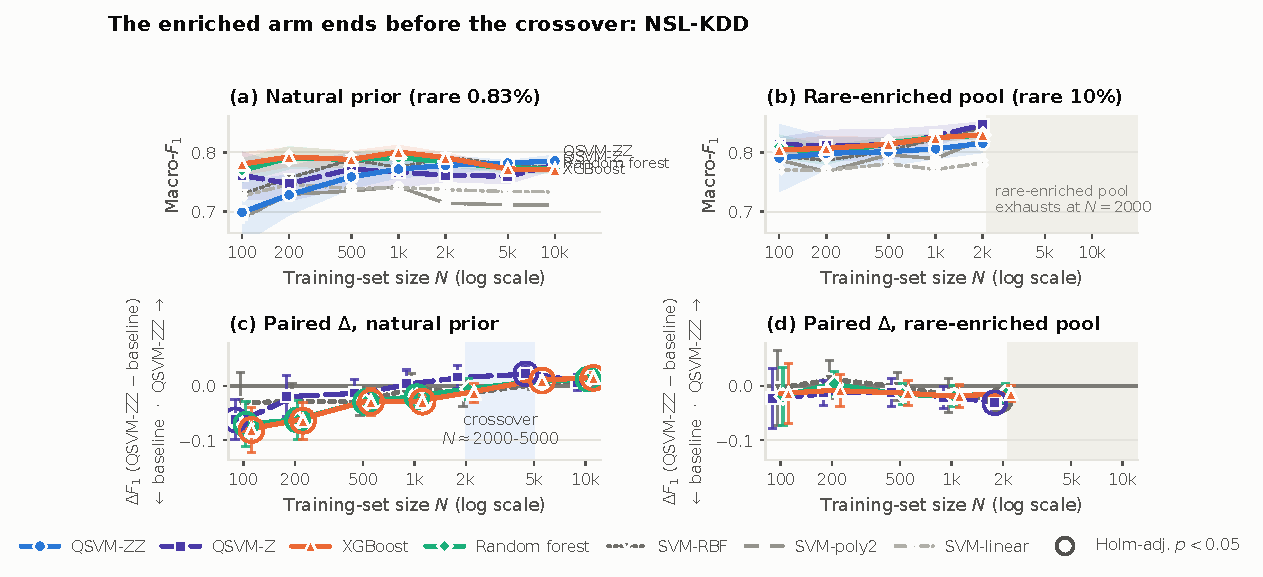
\includegraphics[width=\textwidth]{figs_revision/fig9_learning_curve_nslkdd.pdf}
  \caption{%
    \textbf{Under the natural prior the ordering reverses between $N=2000$ and
    $N=5000$; the rare-enriched arm ends before that interval.} (a,~b) Mean
    macro-$F_1$ over ten runs on the full KDDTest+ set with $95\%$ bands;
    (c,~d) paired differences against each baseline, circled where the
    Holm-adjusted $p<0.05$. The reversal against the tree ensembles and the
    linear and polynomial kernels lies in the band in (c); against SVM-RBF the
    sign change is $+0.0008$ and never significant. The enriched pool (b,~d)
    cannot be sampled past $N=2000$ without runs sharing rare samples, so it
    stops one step before the reversal; within the shared range the tree
    ensembles lead under both priors. Whether enrichment removes the reversal is
    therefore untested, not shown (Sec.~\ref{sec:res-c4}).}
  \label{fig:learning-curve}
\end{figure*}

\input{tables/ref_arm}
\begin{revbody}



The submitted version claimed an advantage in the low-data regime from a sweep
that stopped at $N=1000$. Extending it to $N=10^4$ under the natural class prior
reverses the claim and, in doing so, produces the paper's main new finding
(Fig.~\ref{fig:learning-curve}).

All seven models share the four-component front-end of
Sec.~\ref{sec:framework}, so the ranking below is a ranking of learners on
that embedding. At $N=100$ the ranking is XGBoost $0.7802$, random forest $0.7695$,
QSVM-\Zmap{} $0.7613$, SVM-RBF $0.7296$, linear $0.7261$, \QSVM{} $0.6989$: the
quantum kernel is next to last, and the gap to XGBoost, $-0.0812$, is the
largest in the sweep. At $N=10^4$ the ranking is \QSVM{} $0.7855$, QSVM-\Zmap{}
$0.7787$, SVM-RBF $0.7740$, random forest $0.7728$, XGBoost $0.7706$: the
quantum kernel is first among them. The paired difference against XGBoost passes through
zero between $N=2000$ and $N=5000$ ($-0.0129 \rightarrow +0.0100$), and is
corrected-significant at both $N=5000$ ($p_{\text{Holm}}=0.027$, $d_z=1.22$) and
$N=10^4$ ($+0.0149$, $p_{\text{Holm}}=0.0078$, $d_z=1.07$).

Four qualifications keep this from being read as more than it is.

First, the reversal is not an artefact of re-tuning.
Table~\ref{tab:crossover-arms} repeats the sweep with hyper-parameters frozen at
their C2 values instead of re-tuned at each $N$; all six baseline--arm
combinations change sign in the same interval, $2000\rightarrow5000$. A
re-tuning artefact would not survive freezing the tuning.

Second, the reversal is not uniform across baselines. Against SVM-RBF the
difference does turn positive, but no cell in the sweep reaches
corrected significance; the quantum kernel never demonstrably beats an RBF
kernel at any size we tested. Significance is reached against XGBoost at
$N\geq5000$, against the random forest only at $N=10^4$, and against the linear
and poly-2 kernels from $N=1000$ and $N=2000$ respectively.

Third, whether the reversal is a property of the natural prior cannot be
decided by this design, and an earlier draft of this paper claimed that it was.
Repeating the sweep with rare attacks enriched twelvefold to $10\%$, the
sampling the submitted protocol used, leaves $26$ of $30$ comparisons
inconclusive and shows no crossover in its range; but that range ends at
$N=2000$, because at $N=5000$ the ten runs would share $59\%$ of their rare
samples and independence between runs would be lost, and the crossover under
the natural prior occurs between $N=2000$ and $N=5000$, one step beyond it.
Within the range the two regimes share, the tree ensembles lead under both
priors: against XGBoost the paired difference is negative at all five sizes
under both, against the random forest and SVM-RBF at five of five under the
natural prior and four of five under enrichment, and the sign agrees in $22$ of
the $30$ shared cells; the enriched arm reaches a verdict in $4$ of its $30$
cells against $12$ of $30$ for the natural arm on the same sizes, most of the
difference being classical-favourable cells at $N\leq1000$ that enrichment
leaves inconclusive. The enriched arm therefore ends before the phenomenon begins, and
what the comparison establishes is that enrichment is untested against the
crossover, not that it removes it. What does follow for the submitted protocol
is narrower: a sweep confined to $N\leq2000$, under either prior, could not have
seen the regime in which the kernel does best.

Fourth, the reversal is a statement about the shared embedding, not about the
dataset. Table~\ref{tab:ref-arm} adds a reference arm outside the paired
protocol: XGBoost and the random forest trained on the same nested subsets and
seeds but on all $122$ one-hot features, scored on the same full KDDTest$^+$.
Full-feature XGBoost also declines with $N$ on this split, from
$\refArmXgbPeak$ at $N=\refArmXgbPeakN$ to $\refArmXgbTenK$ at $N=10^4$, and at
$N=5000$ and $N=10^4$ the paired difference against \QSVM{} is
$\refArmDeltaXgbFiveK$ and $\refArmDeltaXgbTenK$: parity, not a crossover.
Against the full-feature random forest the quantum kernel does lead at
$N=10^4$ ($\refArmDeltaRfTenK$). With the entire $125{,}973$-record partition,
full-feature XGBoost reaches $0.804$ (Sec.~\ref{sec:setup}), above the best
score of any four-qubit model in this paper. The practical reading is
therefore narrower than the ranking suggests: a four-qubit kernel matches, but
does not beat, a tree ensemble given the raw record.

\end{revbody}

\subsection{Rare attacks}
\label{sec:res-rare}
\revnote{new}{New subsection. The submitted version claimed ``+6.7 points on rare attacks, d=+0.68'' but the released code computed no rare-class metric (R4-5). That claim is withdrawn.}
\begin{revbody}

Because R2L and U2R are the classes an operator cares about, we report them
separately rather than only inside the macro average. At $N=10^4$ under the
natural prior the rare-class $F_1$ is SVM-RBF $0.585$, \QSVM{} $0.507$,
QSVM-\Zmap{} $0.421$, XGBoost $0.334$, random forest $0.331$, poly-2 $0.109$,
linear $0.089$.

Two things follow. The quantum kernel is far better on rare attacks than either
tree ensemble, which is not visible in the macro average and is worth knowing.
But SVM-RBF is better still, by $0.078$, so the honest statement is that an RBF
kernel is the strongest rare-attack detector in this study. The submitted
version reported a $+6.7$-point rare-attack gain with $d=+0.68$; no rare-class
metric was computed by the code that produced it, and we withdraw the number.
\end{revbody}

\subsection{Transfer to UNSW-NB15}
\label{sec:res-unsw}
\revnote{new}{New subsection. The submitted version mentioned UNSW-NB15 in one sentence of the limitations; AE-3 and R1-2 asked for a second dataset in full.}
\input{figs_revision/fig_unsw_transfer}
\begin{revbody}


The selection rule is applied to UNSW-NB15 without changing a threshold or a
constant (Fig.~\ref{fig:c1-selection}(b)). It returns $n^\ast=6$, at $V=0.9044$,
$\mathrm{KTA}=0.1986$ and $60$ two-qubit gates. Re-running it on ten
independent subsets returns $n^\ast=6$ in $10/10$ at tolerance
$\varepsilon\in\{0.02,0.05\}$ and $7/10$ at $\varepsilon=0.1$. That the rule
returns a different width on a different dataset is the point: it is a rule with
inputs, not a constant dressed as one.

The sample-complexity result does not transfer (Fig.~\ref{fig:unsw-transfer}). At
$N=10^4$, \QSVM{} is favourable against SVM-RBF ($+0.0401$,
$p_{\text{Holm}}=0.0059$) and against its own entanglement-free control
($+0.0449$, $p_{\text{Holm}}=0.0020$), but XGBoost stays ahead at every size
tested ($-0.0204$ at $N=10^4$, classical-favourable), and no crossover against
either tree ensemble occurs anywhere in the sweep. A finding that reproduces on
one dataset and not the other is reported as exactly that.
\end{revbody}

\subsection{Where the kernel breaks, and why}
\label{sec:res-width}
\revnote{new}{New subsection. Answers R3-4 (``very few qubits''): at 8 qubits all 48 comparisons favour the classical side, with the Gram-matrix mechanism measured.}
% Sinh boi runners/make_paper1_figures.py; caption doi chieu bang
% runners/audit_figures.py. File rieng cho tung hinh de \input DUNG CHO
% trong than bai -- float cua LaTeX chi troi VE SAU, khai bao het o cuoi
% tai lieu thi ca 9 hinh don xuong cuoi va tran vao danh muc tai lieu.

\begin{figure*}[t]
  \centering
  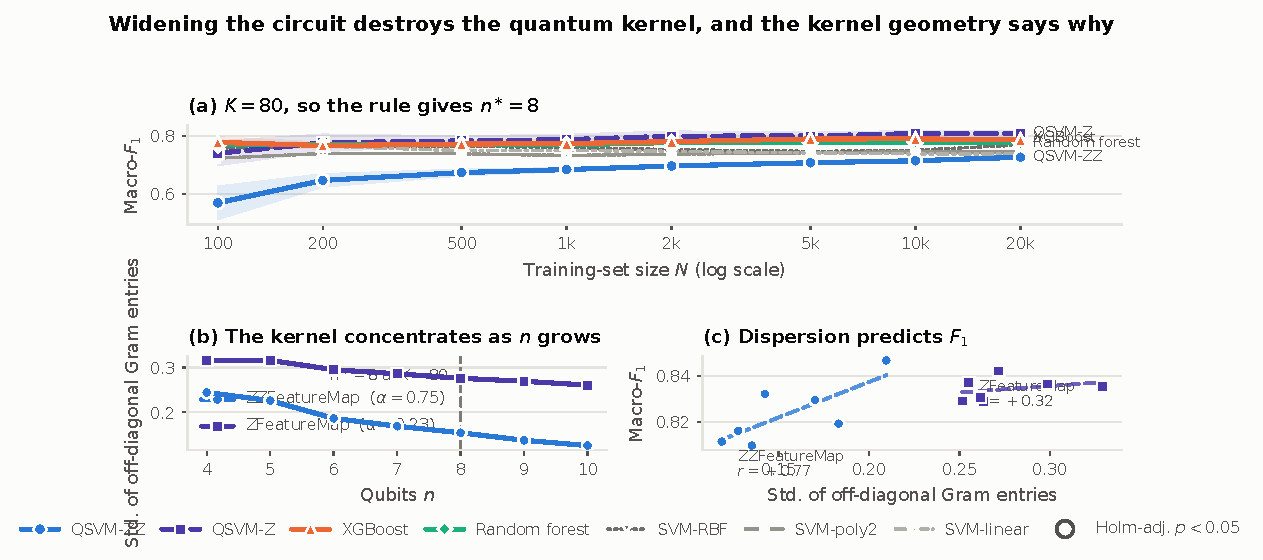
\includegraphics[width=\textwidth]{figs_revision/fig12_width_concentration.pdf}
  \caption{%
    \textbf{Widening the circuit destroys the quantum kernel, and the kernel
    geometry says why.} (a) The sample-complexity sweep re-run at $K=80$, where
    the rule returns $n^{\ast}=8$: all $48$ paired comparisons are
    classical-favourable. (b) Off-diagonal Gram dispersion against width, fitted
    as $n^{-\alpha}$ at $K=80$; the \ZZ{} map concentrates $3.3$ times as fast
    as the \Zmap{} map here ($\alpha=0.75$ against $0.23$), against the factor
    of $2.02$ at $K=20$ that phase-term counting predicts (Sec.~\ref{sec:res-width}).
    (c) Across widths the dispersion correlates with macro-$F_1$ at $r=+0.77$
    for \ZZ{} (95\% CI $[+0.04,+0.96]$) and $r=+0.32$ for \Zmap{}
    ($[-0.57,+0.87]$); the contrast between the two is not resolved at seven
    widths ($z=0.97$, $p=0.33$).}
  \label{fig:width}
\end{figure*}

\begin{revbody}


Sec.~\ref{sec:res-c1} showed that a larger feature budget forces a wider
circuit. Paying that price is the sharpest test of whether the quantum kernel
has headroom, and it fails it (Fig.~\ref{fig:width}).

Re-running the entire sample-complexity sweep at $K=80$, where the rule returns
$n^\ast=8$, produces $48$ paired comparisons (six baselines across eight
training-set sizes), and every one of them is classical-favourable. The
entanglement ablation reverses sign as well: at eight qubits \QSVM{} falls
\emph{below} its entanglement-free control at every size, by $0.082$ to $0.171$
macro-$F_1$. Widening the circuit does not extend the advantage; it removes it.

The mechanism is measurable in the Gram matrix rather than inferred. Writing
$s(n)$ for the standard deviation of the off-diagonal entries and fitting
$s(n)\propto n^{-\alpha}$ over $n=4,\dots,10$, we obtain $\alpha_{\ZZ}=0.590$
against $\alpha_{\Zmap}=0.292$ at $K=20$, a ratio of $2.02$. That ratio is
what the circuit structure predicts: the \ZZ{} map contributes
$\binom{n}{2}$ pairwise phase terms where the \Zmap{} map contributes $n$
single-qubit terms, so the former's phase content grows quadratically and the
latter's linearly. The prediction holds at $K=20$ and not at $K=80$, the budget
at which the collapse occurs: there the fitted exponents are $0.75$ against
$0.23$, a ratio of $3.32$ (Fig.~\ref{fig:width}b), and over the same range the
\ZZ{} kernel loses $49\%$ of its off-diagonal dispersion against $18\%$ for the
\Zmap{} kernel. The counting argument therefore predicts the ordering of the
two decay rates everywhere and their ratio only where the kernel does not
collapse; Sec.~\ref{sec:limitations} returns to this.

The concentration is not merely present; it tracks the end-task result. Across
$n=4,\dots,10$ the correlation between off-diagonal dispersion and macro-$F_1$
is $r=+0.77$ for the \ZZ{} kernel (95\% CI $[+0.04,+0.96]$, $p=0.04$ on seven
widths) and $r=+0.32$ for the \Zmap{} kernel ($[-0.57,+0.87]$, $p=0.48$), which
barely concentrates. The first correlation is resolved, barely; the contrast
between the two is not: a test of the difference between the two correlations
gives $z=0.97$, $p=0.33$, so the data do not establish that the relation is
specific to the concentrating map, and we do not claim that they do. As the Gram
matrix flattens, accuracy follows it down.
This is the exponential-concentration phenomenon of \cite{thanasilp2024} in a
concrete applied setting, and it is why we present a bounded operating window
rather than a method that scales.

An independent measurement supports the boundary and sharpens its
interpretation. Cirillo \emph{et al.} \cite{qmi2026}, sweeping qubit count on
the same corpus under backend-derived noise, locate good performance in a
$20$--$35$ two-qubit-gate band with degradation beyond roughly $60$ gates. Our
operating point of $24$ gates sits inside that band and our collapse at $112$
gates lies beyond their threshold, so the two studies agree on where the
usable window ends. They differ on why: that study attributes the degradation
to two-qubit gate error accumulating on hardware, whereas the results above are
obtained under exact, noiseless simulation, in which no gate error exists. The
window therefore does not widen with better hardware. It is set by the kernel.
\end{revbody}


% =====================================================================
\section{Regime Map: When to Use \QSVM{}}
\label{sec:regimemap}
% =====================================================================
%  VI. Regime Map
%
%  Muc nay la cho "doi khung": tu "chung toi co loi the" sang "day la ranh
%  gioi". So 21/21/68 phai xuat hien nguyen ven, khong duoc chi ke 21 thang.
%  Nguon: results/nslkdd/regime_map_rows.csv, doi chieu ca 110 dong bang
%  runners/audit_c4.py muc E.
% =====================================================================



% Sinh boi runners/make_paper1_figures.py; caption doi chieu bang
% runners/audit_figures.py. File rieng cho tung hinh de \input DUNG CHO
% trong than bai -- float cua LaTeX chi troi VE SAU, khai bao het o cuoi
% tai lieu thi ca 9 hinh don xuong cuoi va tran vao danh muc tai lieu.

\begin{figure*}[t]
  \centering
  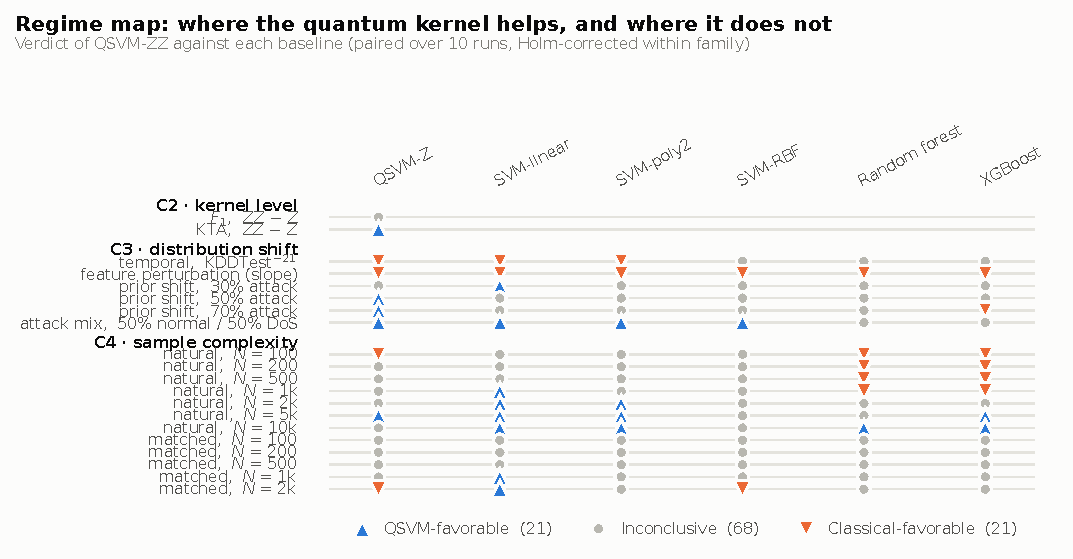
\includegraphics[width=\textwidth]{figs_revision/fig10_regime_map.pdf}
  \caption{%
    \textbf{Regime map: 110 controlled comparisons of \QSVM{} against six
    baselines.} Each cell is one paired comparison over ten runs, Holm-corrected
    within its baseline family (families of one to three; the $20$ cells
    against QSVM-\Zmap{} are uncorrected). Verdicts are encoded by both colour
    and glyph so the figure survives greyscale printing. The distribution is the
    result: $21$ favourable, $21$ classical-favourable, $68$ inconclusive within
    families; $17$, $15$ and $78$ under one Benjamini--Hochberg correction over
    all $110$ cells; and under Holm over all $110$ no cell survives. The seven
    C4-natural rows ($42$ cells) are the single-protocol block of
    Sec.~\ref{sec:regimemap}; the C2 and C3 rows are scored on a $300$- or
    $1000$-record test set. A single aggregate number would hide exactly the
    structure this paper is about.}
  \label{fig:regime-map}
\end{figure*}


Collecting every controlled comparison in one place gives the map in
Fig.~\ref{fig:regime-map}: $110$ cells, each a paired comparison between
\QSVM{} and one baseline under one condition, each carrying a Holm-corrected
verdict. Twenty-one favour the quantum kernel, twenty-one favour a classical
baseline, and sixty-eight are inconclusive. Two qualifications attach to that
count. The cells are corrected within families of one to three
(Sec.~\ref{sec:stats}); under a single Benjamini--Hochberg correction over all
$110$ cells the tally is $17$, $15$ and $78$, every cell that changes moving to
inconclusive and none changing side, and under Holm over all $110$ no cell
survives. And the cells come from two protocols that Sec.~\ref{sec:setup} says
are not interchangeable: $42$ cells from the natural prior on the full
KDDTest$^+$ partition (11 favourable, 9 unfavourable, 22 inconclusive) and $68$
from the rare-enriched pool (10, 12, 46), of which $30$ are scored on the full
partition and $38$ on a $300$-record or re-mixed $1000$-record test set. A
difference estimated on $300$ records and one estimated on $22{,}544$ do not
carry the same weight, and the reader who wants a single-protocol map should
read the natural-prior block on its own.

The balance of the first two numbers is the honest summary of this study. A
practitioner reading only the count would conclude that the quantum kernel is
neither better nor worse on average, and that conclusion would be correct and
useless. The map is worth more than its margin because the verdicts are not
distributed at random across conditions.

\subsection{Where it is worth the cost}
\revnote{rewrite}{The submitted forest plot had 9 rows; now 110 cells, each with $\Delta$, CI, $p$ and $d_z$ (R2-4).}
\begin{revbody}

Three conditions produce a favourable verdict, and they share a structure.

\emph{Enough data, natural prior.} At $N\geq5000$ under the natural class prior,
\QSVM{} is favourable against XGBoost and, at $N=10^{4}$, against the random
forest; it is favourable against the linear and poly-2 kernels from $N=1000$ and
$N=2000$. Below $N=2000$ the verdicts run the other way. The regime is bounded
on both sides: below it the kernel has too little data, and
Sec.~\ref{sec:res-width} shows that a wider circuit does not extend it upward.
It is also bounded from above by a model outside the paired protocol: every
favourable verdict here is against a baseline given the same four components,
and against XGBoost given all $122$ features the kernel reaches parity at
$N\geq5000$ (Table~\ref{tab:ref-arm}), while XGBoost on the full training
partition scores $0.804$, above any four-qubit model in this paper
(Sec.~\ref{sec:setup}). The regime is where the kernel is worth its cost
relative to a classical learner on the same embedding, not relative to the best
classical score available on the record.

\emph{Balanced binary composition.} On a $50/50$ Normal--DoS mixture the quantum
kernel is favourable against all four kernel baselines, with effect sizes up to
$3.02$. This is a C3 cell: models trained on the rare-enriched $N=1000$ pool
and scored on a re-mixed $1000$-record test set, so it lies outside the
natural-prior block and is not visible in the single-protocol reading. This is the condition under which quantum-kernel IDS results are most
often reported in the literature, and our numbers reproduce that impression;
which is part of why we report the other conditions too.

\emph{Rare-attack detection relative to tree ensembles.} At $N=10^{4}$ the
rare-class $F_{1}$ of \QSVM{} is $0.507$ against $0.334$ for XGBoost and $0.331$
for the random forest. If the deployment objective is rare-attack recall rather
than macro-averaged accuracy, the ranking changes substantially, though
SVM-RBF, at $0.585$, remains ahead of both.
\end{revbody}

\subsection{Where it is not}
\revnote{rewrite}{R2-4 observed that favourable regimes received full statistics and unfavourable ones only qualitative remarks; both sides now receive the same treatment.}
\begin{revbody}

\emph{Small training sets.} At $N\leq500$ the quantum kernel loses to both tree
ensembles at every size, by up to $0.081$ macro-$F_{1}$. No configuration we
tested recovers this.

\emph{Feature perturbation.} Six of six comparisons are classical-favourable
with effect sizes beyond $2.8$. The quantum kernel is the most perturbation-%
sensitive model in the study, which matters for a security application where
adversarial feature manipulation is the norm rather than the exception. Like
the balanced-composition result above, this is a C3 cell on the rare-enriched
pool and a $1000$-record test set, outside the natural-prior block; the two
clearest effect sizes in the map both come from that protocol.

\emph{Strong prior shift.} At a $70\%$ attack rate the comparison against
XGBoost is classical-favourable, and \QSVM{} degrades across the shift by
$0.032$ against $0.021$ for XGBoost. The submitted version presented this regime
as its strongest evidence; against strong tabular baselines it is evidence in
the opposite direction.

\emph{Wide circuits.} At $K=80$ and $n^{\ast}=8$, all $48$ comparisons are
classical-favourable. This is the sharpest boundary we found and the least
expected: it says the operating window is closed from above by the physics of
the feature map rather than by engineering limits that better hardware would
lift.

\emph{Any comparison against SVM-RBF on sample size.} Across the whole sweep, no
cell reaches corrected significance in the quantum kernel's favour. An RBF
kernel is the baseline this method does not clear.
\end{revbody}

\subsection{Reading the map}
\revnote{new}{New subsection, absorbing the ``decision rule'' of the submitted version.}
\begin{revbody}

Two properties of the map should govern how it is generalised.

First, the inconclusive cells are the majority, and they are informative. With
ten runs and Holm correction the smallest difference that reaches a verdict
anywhere in the map is $0.010$ macro-$F_1$, while differences as large as
$0.031$ remain inconclusive when their run-to-run spread is wide; the median
inconclusive cell sits at $0.014$. Most of the differences in this study are of
that order. A study reporting sharper verdicts on the same data with fewer
repetitions and no multiplicity control is not seeing more; it is resolving
less.

Second, the favourable regime is bounded on every axis we varied, and the
bounds are not far apart: $N \gtrsim 5000$ but not at a width beyond four to six
qubits, on NSL-KDD but not on UNSW-NB15 for the sample-size effect, and under
the natural prior, with the enriched prior untested at the sizes where the
regime lies. A method whose advantage is confined to a
box this small is not yet a practical instrument, and we do not present it as
one. What it is, on this evidence, is a phenomenon with a measurable boundary
and the boundary, being predicted by the circuit's phase-term count, is the
part most likely to hold beyond these two datasets.
\end{revbody}


% =====================================================================
% =====================================================================
%  Muc VII viet lai -- TETC-2026-05-0252
%
%  Ban da nop hua ba thu la "ongoing work" hoac "deferred": (a) do tac dong
%  cua be rong mach, (b) so voi baseline khong phai SVM, (c) dataset thu hai.
%  Ca ba nay bay gio deu co so do, nen muc han che khong con la loi hua ma la
%  bao cao ket qua kem ranh gioi ro rang.
%
%  Cho DUY NHAT van con la loi hua: thuc thi tren QPU that. Phai ghi that ro
%  da lam gi va CHUA lam gi -- neu de mo ho thi reviewer se doc "NISQ-aware"
%  thanh mot khang dinh ve phan cung ma bai khong do duoc.
% =====================================================================

\section{Limitations and Threats to Validity}
\label{sec:limitations}

\subsection{Hardware noise: what was and was not measured}
\revnote{rewrite}{The submitted version covered finite-shot error only. A backend-derived noise model is added (AE-6, R1-6, R3-4), with a statement of what is not measured.}
\begin{revbody}

The submitted version reported only finite-shot sampling error and deferred
coherent noise to a companion study. Reviewers correctly objected that shot
noise alone cannot support a NISQ-feasibility claim. We therefore state the
scope precisely.

\emph{What we measure.} The C2 pipeline is re-run under a noise model derived
from the published calibration data of a real superconducting backend
(\texttt{FakeManilaV2}) \cite{ref27} via \texttt{NoiseModel.from\_backend}, which
carries gate errors, readout errors, and gate-duration-dependent thermal
relaxation.
Circuits are transpiled onto that backend's coupling map and basis gate set,
giving a depth of $59$ and $44$ two-qubit gates for the $n=4$, $r=2$ map.
Under this model the entanglement conclusion is unchanged: the alignment gap
between QSVM-ZZ and QSVM-Z survives, while the macro-$F_1$ difference remains
within its confidence interval. This noisy re-run covers one of the ten runs
and the $300$-record test split (Table~\ref{tab:protocol}); it establishes
that the noise model does not move the operating point, not a noisy confidence
interval, which would require the remaining nine runs at the same $512$ shots
per kernel entry.

\emph{What we do not measure.} The circuits were not executed on a quantum
processor. Two effects are therefore outside our evidence: drift of calibration
parameters between the snapshot and execution time, and idle-time decoherence
beyond what gate durations already attribute. Our released code contains the
execution path for a real backend, and the comparison it would produce
(exact statevector $\rightarrow$ backend-derived noise $\rightarrow$ hardware)
is specified, but we report no hardware numbers and make no claim about them.
Readers should read ``NISQ-aware'' as a statement about \emph{circuit budget}
(qubit count, depth, and two-qubit gate count chosen under an explicit cost
model, in the sense of \cite{ref8}) and not as a claim of hardware validation.
\end{revbody}

\subsection{Embedding size: now measured, and the news is not good for width}
\revnote{fix}{The submitted version left this as an ``open question''; it is now measured, and the result is unfavourable to wider circuits.}
\begin{revbody}

The submitted version listed the effect of moving along the frontier as an open
question. We have since measured it, and the answer constrains the method more
sharply than we expected.

Increasing the feature budget $K$ does buy accuracy for a classical proxy, but
it is not free: retaining $85\%$ of the variance at $K=80$ requires $n^\ast=8$
qubits rather than the $n^\ast=4$ that $K=20$ admits, raising the two-qubit gate
count from $24$ to $112$. Re-running the full sample-complexity sweep at that
operating point removes the quantum kernel's advantage entirely: across eight
training-set sizes and six baselines, all $48$ paired comparisons favour the
classical model, and the entanglement ablation reverses sign, with QSVM-ZZ now
\emph{below} its entanglement-free control.

The mechanism is measurable rather than conjectural. The dispersion of the
off-diagonal Gram entries decays with width as $n^{-\alpha}$, and the fitted
exponent for the ZZ map is close to twice that of the Z map at $K=20$
($0.59$ vs.\ $0.29$), consistent with the $\binom{n}{2}$ pairwise phase terms of
the former growing quadratically where the latter's grow linearly. Across
$n=4$ to $10$ the macro-$F_1$ of the ZZ kernel tracks this dispersion
($r=+0.77$, 95\% CI $[+0.04,+0.96]$), whereas the Z kernel, which barely
concentrates, shows no resolved dependence ($r=+0.32$, $[-0.57,+0.87]$). This is
the concentration phenomenon of \cite{thanasilp2024} appearing directly in our
setting.

Three caveats. The exponent ratio is $2.02$ at $K=20$, where the kernel does not
collapse, and $3.32$ at $K=80$, where it does, so the term-counting argument
predicts the ordering of the two rates and, at the collapse, not their ratio;
the abstract and Sec.~\ref{sec:intro} state both values. The $F_1$--dispersion
relation is measured on seven widths at a single training-set size, and the
contrast between the two kernels' correlations is not resolvable at seven
points ($z=0.97$, $p=0.33$); we present the relation as an empirical regularity
of the \ZZ{} map, not a law, and make no claim that it is specific to the
concentrating map. A test of either would need more widths and more than one
training-set size.
\end{revbody}

\subsection{Classical-baseline strength}
\revnote{rewrite}{RF and XGBoost added; CatBoost, TabNet and FT-Transformer deliberately not added, with the reason stated (R1-5).}
\begin{revbody}

The submitted version compared only against SVM variants. We have added a
random forest and XGBoost under the identical protocol, and they change the
headline: on the main benchmark XGBoost attains the highest mean macro-$F_1$
($0.8503$) ahead of QSVM-ZZ ($0.8469$), with overlapping intervals. We report
this as an ordering of point estimates, not a significant separation.

We did not add CatBoost or deep tabular models such as TabNet and
FT-Transformer. CatBoost would supply a second gradient-boosting representative
without changing the comparison structure; the deep tabular family would require
its own tuning-budget protocol to be compared fairly, which would enlarge the
study from a controlled quantum-kernel benchmark into a survey of tabular
architectures. We therefore do not claim coverage of all strong tabular methods,
and any practical reading of our results should be qualified accordingly.
\end{revbody}

\subsection{Dataset breadth and protocol}
\revnote{rewrite}{UNSW-NB15 added, with duplication statistics for both corpora.}
\begin{revbody}

The submitted version rested almost entirely on NSL-KDD. We have added
UNSW-NB15 under the same protocol, which is what allows us to separate findings
that transfer from findings that do not: the dimension-selection rule and the
entanglement ablation transfer, while the sample-complexity crossover and the
rare-class behaviour do not.

Two properties of the data limit what either dataset can show. NSL-KDD is an
aging benchmark in which $610$ test rows are identical to a training row in both
features and label ($617$ match on features alone). UNSW-NB15 is far more heavily
duplicated: $47.3\%$ of training rows are internal repeats, and $25.0\%$ of test
rows have an exact duplicate in the training partition, which
inflates absolute scores. Our claims are paired differences between models
evaluated on the same rows, which removes the duplication from the level but
not necessarily from the comparison: a tree ensemble reproduces an exact
training row by construction, a fidelity-kernel SVM does so only through its
support vectors and regulariser, and on the quarter of the UNSW-NB15 test set
that duplicates a training row a paired difference may therefore measure
memorisation rather than generalisation. We have not re-scored the paired
differences on the de-duplicated test subsets, because the sweep's per-row
predictions were not retained, and we list that re-scoring as the one cheap
check this study owes: until it is done, the UNSW-NB15 verdicts, and to a
smaller degree the NSL-KDD ones, carry this threat, and the absolute numbers
are not comparable to studies that de-duplicate.

Finally, the feature budget $K=20$ is inherited from the submitted protocol and
held fixed so that the revised results remain comparable to it.
Fig.~\ref{fig:ksweep} shows it is not the accuracy optimum; it is the value at
which the selection rule returns a four-qubit circuit.
\end{revbody}
            % Sec VII, da co \section ben trong

% =====================================================================
\section{Conclusion and Future Work}
\label{sec:conclusion}
% =====================================================================
%  VIII. Conclusion
%
%  Khong duoc ket bang "ket qua hua hen". Ket bang cai ta do duoc va cai
%  ta khong do duoc. Cau cuoi cung phai la mot cau kiem chung duoc.
% =====================================================================

\revnote{rewrite}{Rewritten: the advantage claim is replaced by the boundary the regime map draws (AE-1, R1-4, R3-2).}
\begin{revbody}
We set out to locate, rather than to demonstrate, the value of a NISQ-feasible
quantum kernel for network intrusion detection. Varying one factor at a time
over $110$ controlled comparisons, we find $21$ verdicts favouring the quantum
kernel, $21$ favouring a classical baseline, and $68$ inconclusive when each
is corrected within its baseline family; $17$, $15$ and $78$ under one
Benjamini--Hochberg correction over the map; and no surviving verdict at all
under Holm over all $110$ cells. Inside that balance there is a structure that
a single-operating-point benchmark cannot see, and it is stated below with the
protocol each part of it comes from.

The structure has three parts. The ordering between \QSVM{} and the tree
ensembles and the linear and polynomial kernels reverses between $N=2000$ and
$N=5000$ under the natural class prior, in both tuning arms, on a shared
four-component embedding; it does not demonstrably reverse against SVM-RBF at
any size tested, it becomes parity rather than a lead against XGBoost on the raw
$122$ features, and whether rare-attack enrichment removes it is not decided by
this design, whose enriched arm ends before the reversal begins. A
lexicographic selection rule that charges for two-qubit gates returns
$n^{\ast}=4$ on NSL-KDD and $n^{\ast}=6$ on UNSW-NB15 without any change of
threshold, so the embedding dimension is a property of the dataset rather than a
constant to be inherited. And the operating window is closed from above: at
$K=80$, where the rule requires eight qubits, every one of $48$ comparisons
favours the classical model, with off-diagonal Gram dispersion decaying faster
for the \ZZ{} map than for its entanglement-free control, by the factor of two
that phase-term counting predicts at $K=20$ and by $3.3$ at $K=80$, and tracking
macro-$F_1$ at $r=+0.77$ over seven widths (95\% CI $[+0.04,+0.96]$).

That last result is the one we would most like others to test. It ties a
structural property of the circuit ($\binom{n}{2}$ pairwise phase terms
against $n$ single-qubit ones) to a decay exponent we can measure and to an
end-task metric that follows it down. If it holds on other corpora and other
maps, then the practical question for quantum kernels on tabular data is not how
to make them more expressive but how to keep them from concentrating, and the
useful width is bounded well below where hardware limits bite.

We are equally clear about what this study does not establish. The circuits were
not executed on a quantum processor, and ``NISQ-aware'' here means a circuit
budget chosen under an explicit cost model, not hardware validation. The
comparison covers two datasets, two tree ensembles and three kernel baselines,
not the deep tabular architectures. The favourable regime is narrow on every
axis we varied. And five claims from the earlier version of this work do not
survive the revised protocol; they are withdrawn in Sec.~\ref{sec:intro} and
corrected in Sec.~\ref{sec:erratum}.

Three directions follow directly. Executing the same kernels on hardware would
close the one gap our simulations cannot: the released code contains the
execution path and the three-tier comparison it would produce is already
specified. Testing the dispersion--accuracy relationship on projected quantum
kernels, which concentrate differently, would show whether the boundary we
measured is a property of fidelity kernels specifically or of the approach.
And since the crossover reproduces on one dataset and not the other, the
mechanism behind it, why more data helps this kernel more than it helps a
tree ensemble and only under a skewed prior, remains open. Our full
implementation, protocol files, intermediate artifacts and two independent audit
scripts are released so that each of these can be started from where we stopped.
\end{revbody}


% =====================================================================
%  Phu luc: chung minh Lemma 1. Ban da nop hua "Appendix A" nhung IEEEtran
%  can \appendices tuong minh -- lenh do nam trong file duoi.
% =====================================================================
\input{sections/09_appendix}

% =====================================================================
\section*{Acknowledgment}
This work was supported by The University of Danang - University of Science
and Technology, project T2026-02-10TN. The authors thank Danang Architecture
University for computing resources, and the maintainers of Qiskit and
scikit-learn.
\begin{revbody}
The authors used Anthropic's Claude (Opus~5) as an assistant during the
preparation of this revision. Its use covered three areas: drafting and editing
prose throughout the manuscript and the response letter; writing the analysis,
audit and experiment-orchestration scripts released with the artifact; and
proposing measurements reported in Secs.~IV and~V, among them the symmetric
tuning arms, the protocol-by-contribution table, the full-feature reference arm
(Table~IV) and the audit scripts. All experimental results were produced by
executing the released code, and every number reported here was checked
against the run records by the authors, who take full responsibility for the
content of this paper.
\end{revbody}

% =====================================================================
%  Danh muc tai lieu. TUNG co \clearpage o day lam chot chan chong hinh
%  xen vao giua cac muc tai lieu; da bo vi nguyen nhan goc (ca 9 hinh khai
%  bao o cuoi tai lieu) da sua, va chot chan do lam trong nua trang truoc
%  phan References.
% =====================================================================
% =====================================================================
\input{bibliography}           % 35 muc; xem ghi chu trong file

% 13/09/2026: tieu su 5 tac gia (TETC yeu cau trong ban revise; ban da nop co)
\input{sections/10_biographies}
 va % =====================================================================
%  PREAMBLE dung chung cho ca hai ban:
%    main_revision.tex   -> ban SACH (nop cho tap chi)
%    main_annotated.tex  -> ban CO DANH DAU (de thay va AE doi chieu)
%  Sua o day thi ca hai ban cung doi -- khong co ban nao lech ban nao.
% =====================================================================

% =====================================================================
%  TETC-2026-05-0252 -- BAN REVISION
%
%  Dung lai tu paper1.pdf vi file .tex goc khong con. Tieu de, danh sach
%  tac gia va don vi GIU NGUYEN: IEEE cam doi tac gia neu khong co dong y
%  bang van ban cua EiC, va reviewer trich dan theo so muc cu.
%
%  Bien dich:  pdflatex -> pdflatex   (bibliography la thebibliography,
%              khong can BibTeX)
%
%  Cac manh duoc \input o duoi deu co the kiem doc lap:
%      python runners/audit_c4.py        -> 100/100
%      python runners/audit_figures.py   ->  36/36
% =====================================================================

\usepackage{cite}
\usepackage{amsmath,amssymb,amsfonts}
\usepackage{amsthm}
\usepackage{algorithmic}
\usepackage{graphicx}
\usepackage{textcomp}
\usepackage{xcolor}
\usepackage{booktabs}
\usepackage{multirow}
\usepackage{array}
\usepackage{url}
\usepackage{bm}
\usepackage[hidelinks]{hyperref}

\graphicspath{{./}}

% =====================================================================
%  Tham so dat float. Mac dinh cua LaTeX chi cho float chiem <=70% dinh
%  trang va bat chua >=20% chu, nen hinh rong ca trang gan nhu luon bi day
%  di cho khac; day du xa thi no roi xuong cuoi bai va xen vao danh muc tai
%  lieu. Noi rong ra thi hinh dat duoc ngay trang no duoc nhac toi.
% =====================================================================
\setcounter{topnumber}{2}
\setcounter{bottomnumber}{1}
\setcounter{totalnumber}{3}
\setcounter{dbltopnumber}{2}
\renewcommand{\topfraction}{0.92}
\renewcommand{\bottomfraction}{0.5}
\renewcommand{\textfraction}{0.07}
\renewcommand{\floatpagefraction}{0.80}
\renewcommand{\dbltopfraction}{0.92}
\renewcommand{\dblfloatpagefraction}{0.80}

% Trang chi co float: mac dinh LaTeX can giua theo chieu doc, nen hai hinh
% bi keo xa nhau bang mot khoang trang lon. Ep can tren, khoang cach co
% dinh, phan du don xuong duoi.
\makeatletter
\setlength{\@fptop}{0pt}
\setlength{\@fpsep}{10pt plus 1fil}
\setlength{\@fpbot}{0pt plus 2fil}
\setlength{\@dblfptop}{0pt}
\setlength{\@dblfpsep}{10pt plus 1fil}
\setlength{\@dblfpbot}{0pt plus 2fil}
\makeatother

% Moi truong dinh ly. Ban da nop dung Proposition cho ca nhung su that hien
% nhien; ban nay chi con Lemma (dan xuat rieng cua bai) va Definition.
\newtheorem{definition}{Definition}
\newtheorem{lemma}{Lemma}
\newtheorem{assumption}{Assumption}
\newtheorem{problem}{Problem}
\theoremstyle{remark}
\newtheorem{remark}{Remark}

\newcommand{\ZZ}{\textsc{zz}}
\newcommand{\Zmap}{\textsc{z}}
\newcommand{\QSVM}{QSVM-\ZZ}
\newcommand{\Fmac}{F_1^{\mathrm{macro}}}

% =====================================================================
%  DANH DAU THAY DOI so voi ban da nop (TETC bat buoc nop ban danh dau).
%
%  Mot nguon, hai ban:
%    main_revision.tex   -> ban SACH, khong hien gi
%    main_annotated.tex  -> bat co \annottrue, hien nhan o le trai
%
%  Dung \revnote{loai}{ghi chu} ngay sau moi \subsection. Cac loai:
%    new      muc hoan toan moi, ban da nop khong co
%    rewrite  co trong ban cu nhung viet lai
%    fix      SUA LOI cua ban cu
%    keep     giu nguyen y cua ban cu
% =====================================================================
% \newif\ifannot -- 13/09: dinh nghia + dat co o main_revision.tex / main_annotated.tex TRUOC % =====================================================================
%  PREAMBLE dung chung cho ca hai ban:
%    main_revision.tex   -> ban SACH (nop cho tap chi)
%    main_annotated.tex  -> ban CO DANH DAU (de thay va AE doi chieu)
%  Sua o day thi ca hai ban cung doi -- khong co ban nao lech ban nao.
% =====================================================================

% =====================================================================
%  TETC-2026-05-0252 -- BAN REVISION
%
%  Dung lai tu paper1.pdf vi file .tex goc khong con. Tieu de, danh sach
%  tac gia va don vi GIU NGUYEN: IEEE cam doi tac gia neu khong co dong y
%  bang van ban cua EiC, va reviewer trich dan theo so muc cu.
%
%  Bien dich:  pdflatex -> pdflatex   (bibliography la thebibliography,
%              khong can BibTeX)
%
%  Cac manh duoc \input o duoi deu co the kiem doc lap:
%      python runners/audit_c4.py        -> 100/100
%      python runners/audit_figures.py   ->  36/36
% =====================================================================

\usepackage{cite}
\usepackage{amsmath,amssymb,amsfonts}
\usepackage{amsthm}
\usepackage{algorithmic}
\usepackage{graphicx}
\usepackage{textcomp}
\usepackage{xcolor}
\usepackage{booktabs}
\usepackage{multirow}
\usepackage{array}
\usepackage{url}
\usepackage{bm}
\usepackage[hidelinks]{hyperref}

\graphicspath{{./}}

% =====================================================================
%  Tham so dat float. Mac dinh cua LaTeX chi cho float chiem <=70% dinh
%  trang va bat chua >=20% chu, nen hinh rong ca trang gan nhu luon bi day
%  di cho khac; day du xa thi no roi xuong cuoi bai va xen vao danh muc tai
%  lieu. Noi rong ra thi hinh dat duoc ngay trang no duoc nhac toi.
% =====================================================================
\setcounter{topnumber}{2}
\setcounter{bottomnumber}{1}
\setcounter{totalnumber}{3}
\setcounter{dbltopnumber}{2}
\renewcommand{\topfraction}{0.92}
\renewcommand{\bottomfraction}{0.5}
\renewcommand{\textfraction}{0.07}
\renewcommand{\floatpagefraction}{0.80}
\renewcommand{\dbltopfraction}{0.92}
\renewcommand{\dblfloatpagefraction}{0.80}

% Trang chi co float: mac dinh LaTeX can giua theo chieu doc, nen hai hinh
% bi keo xa nhau bang mot khoang trang lon. Ep can tren, khoang cach co
% dinh, phan du don xuong duoi.
\makeatletter
\setlength{\@fptop}{0pt}
\setlength{\@fpsep}{10pt plus 1fil}
\setlength{\@fpbot}{0pt plus 2fil}
\setlength{\@dblfptop}{0pt}
\setlength{\@dblfpsep}{10pt plus 1fil}
\setlength{\@dblfpbot}{0pt plus 2fil}
\makeatother

% Moi truong dinh ly. Ban da nop dung Proposition cho ca nhung su that hien
% nhien; ban nay chi con Lemma (dan xuat rieng cua bai) va Definition.
\newtheorem{definition}{Definition}
\newtheorem{lemma}{Lemma}
\newtheorem{assumption}{Assumption}
\newtheorem{problem}{Problem}
\theoremstyle{remark}
\newtheorem{remark}{Remark}

\newcommand{\ZZ}{\textsc{zz}}
\newcommand{\Zmap}{\textsc{z}}
\newcommand{\QSVM}{QSVM-\ZZ}
\newcommand{\Fmac}{F_1^{\mathrm{macro}}}

% =====================================================================
%  DANH DAU THAY DOI so voi ban da nop (TETC bat buoc nop ban danh dau).
%
%  Mot nguon, hai ban:
%    main_revision.tex   -> ban SACH, khong hien gi
%    main_annotated.tex  -> bat co \annottrue, hien nhan o le trai
%
%  Dung \revnote{loai}{ghi chu} ngay sau moi \subsection. Cac loai:
%    new      muc hoan toan moi, ban da nop khong co
%    rewrite  co trong ban cu nhung viet lai
%    fix      SUA LOI cua ban cu
%    keep     giu nguyen y cua ban cu
% =====================================================================
% \newif\ifannot -- 13/09: dinh nghia + dat co o main_revision.tex / main_annotated.tex TRUOC % =====================================================================
%  PREAMBLE dung chung cho ca hai ban:
%    main_revision.tex   -> ban SACH (nop cho tap chi)
%    main_annotated.tex  -> ban CO DANH DAU (de thay va AE doi chieu)
%  Sua o day thi ca hai ban cung doi -- khong co ban nao lech ban nao.
% =====================================================================

% =====================================================================
%  TETC-2026-05-0252 -- BAN REVISION
%
%  Dung lai tu paper1.pdf vi file .tex goc khong con. Tieu de, danh sach
%  tac gia va don vi GIU NGUYEN: IEEE cam doi tac gia neu khong co dong y
%  bang van ban cua EiC, va reviewer trich dan theo so muc cu.
%
%  Bien dich:  pdflatex -> pdflatex   (bibliography la thebibliography,
%              khong can BibTeX)
%
%  Cac manh duoc \input o duoi deu co the kiem doc lap:
%      python runners/audit_c4.py        -> 100/100
%      python runners/audit_figures.py   ->  36/36
% =====================================================================

\usepackage{cite}
\usepackage{amsmath,amssymb,amsfonts}
\usepackage{amsthm}
\usepackage{algorithmic}
\usepackage{graphicx}
\usepackage{textcomp}
\usepackage{xcolor}
\usepackage{booktabs}
\usepackage{multirow}
\usepackage{array}
\usepackage{url}
\usepackage{bm}
\usepackage[hidelinks]{hyperref}

\graphicspath{{./}}

% =====================================================================
%  Tham so dat float. Mac dinh cua LaTeX chi cho float chiem <=70% dinh
%  trang va bat chua >=20% chu, nen hinh rong ca trang gan nhu luon bi day
%  di cho khac; day du xa thi no roi xuong cuoi bai va xen vao danh muc tai
%  lieu. Noi rong ra thi hinh dat duoc ngay trang no duoc nhac toi.
% =====================================================================
\setcounter{topnumber}{2}
\setcounter{bottomnumber}{1}
\setcounter{totalnumber}{3}
\setcounter{dbltopnumber}{2}
\renewcommand{\topfraction}{0.92}
\renewcommand{\bottomfraction}{0.5}
\renewcommand{\textfraction}{0.07}
\renewcommand{\floatpagefraction}{0.80}
\renewcommand{\dbltopfraction}{0.92}
\renewcommand{\dblfloatpagefraction}{0.80}

% Trang chi co float: mac dinh LaTeX can giua theo chieu doc, nen hai hinh
% bi keo xa nhau bang mot khoang trang lon. Ep can tren, khoang cach co
% dinh, phan du don xuong duoi.
\makeatletter
\setlength{\@fptop}{0pt}
\setlength{\@fpsep}{10pt plus 1fil}
\setlength{\@fpbot}{0pt plus 2fil}
\setlength{\@dblfptop}{0pt}
\setlength{\@dblfpsep}{10pt plus 1fil}
\setlength{\@dblfpbot}{0pt plus 2fil}
\makeatother

% Moi truong dinh ly. Ban da nop dung Proposition cho ca nhung su that hien
% nhien; ban nay chi con Lemma (dan xuat rieng cua bai) va Definition.
\newtheorem{definition}{Definition}
\newtheorem{lemma}{Lemma}
\newtheorem{assumption}{Assumption}
\newtheorem{problem}{Problem}
\theoremstyle{remark}
\newtheorem{remark}{Remark}

\newcommand{\ZZ}{\textsc{zz}}
\newcommand{\Zmap}{\textsc{z}}
\newcommand{\QSVM}{QSVM-\ZZ}
\newcommand{\Fmac}{F_1^{\mathrm{macro}}}

% =====================================================================
%  DANH DAU THAY DOI so voi ban da nop (TETC bat buoc nop ban danh dau).
%
%  Mot nguon, hai ban:
%    main_revision.tex   -> ban SACH, khong hien gi
%    main_annotated.tex  -> bat co \annottrue, hien nhan o le trai
%
%  Dung \revnote{loai}{ghi chu} ngay sau moi \subsection. Cac loai:
%    new      muc hoan toan moi, ban da nop khong co
%    rewrite  co trong ban cu nhung viet lai
%    fix      SUA LOI cua ban cu
%    keep     giu nguyen y cua ban cu
% =====================================================================
% \newif\ifannot -- 13/09: dinh nghia + dat co o main_revision.tex / main_annotated.tex TRUOC \input{preamble}
% 13/09/2026: TETC doi ban annotated to NEN VANG phan moi/doi. Moi truong revbody boc than
% moi subsection co nhan new/rewrite/fix; che do sach thi khong lam gi. framed/shaded* qua trang duoc;
% float khong duoc nam trong no (script check/make_yellow_annotated.py da doi \input float ra ngoai).
% 13/09 toi: Hao yeu cau to VANG chu (inline highlight), khong dong khung khoi. Ban annotated bien dich
% bang LUALATEX: lua-ul \highLight to nen tung dong chu, di qua ngat doan, cong thuc, itemize; float da doi ra ngoai.
% Ban sach van bien dich bang pdflatex (revbody khong lam gi). environ bat than moi truong thanh \BODY.
\usepackage{environ}
\ifannot
  \usepackage{luacolor}\usepackage{lua-ul}
  \NewEnviron{revbody}{\highLight[yellow!45]{\BODY}}
\else
  \newenvironment{revbody}{}{}
\fi
\definecolor{tagnew}{HTML}{0B6E4F}
\definecolor{tagrew}{HTML}{1F3D6B}
\definecolor{tagfix}{HTML}{A3341F}
\definecolor{tagkeep}{HTML}{6B6B6B}
\newcommand{\revnote}[2]{%
  \ifannot
    \par\nobreak\vspace{1pt}%
    {\footnotesize\sffamily
     \csname revtag@#1\endcsname~\textcolor{tagkeep}{#2}}%
    \par\nobreak\vspace{2pt}%
  \fi}
\expandafter\def\csname revtag@new\endcsname{%
  \colorbox{tagnew}{\textcolor{white}{\bfseries NEW}}}
\expandafter\def\csname revtag@rewrite\endcsname{%
  \colorbox{tagrew}{\textcolor{white}{\bfseries REWRITTEN}}}
\expandafter\def\csname revtag@fix\endcsname{%
  \colorbox{tagfix}{\textcolor{white}{\bfseries CORRECTED}}}
\expandafter\def\csname revtag@keep\endcsname{%
  \colorbox{tagkeep}{\textcolor{white}{\bfseries RETAINED}}}

% Ten cong khai de dung trong bang chu giai cua main_annotated.tex
\newcommand{\revtagnew}{\csname revtag@new\endcsname}
\newcommand{\revtagrewrite}{\csname revtag@rewrite\endcsname}
\newcommand{\revtagfix}{\csname revtag@fix\endcsname}
\newcommand{\revtagkeep}{\csname revtag@keep\endcsname}



% 13/09/2026: so cua nhanh tham chieu (XGBoost/RF du dac trung), sinh boi check/pair_ref_arm.py
\input{tables/ref_arm_macros}

% 13/09/2026: TETC doi ban annotated to NEN VANG phan moi/doi. Moi truong revbody boc than
% moi subsection co nhan new/rewrite/fix; che do sach thi khong lam gi. framed/shaded* qua trang duoc;
% float khong duoc nam trong no (script check/make_yellow_annotated.py da doi \input float ra ngoai).
% 13/09 toi: Hao yeu cau to VANG chu (inline highlight), khong dong khung khoi. Ban annotated bien dich
% bang LUALATEX: lua-ul \highLight to nen tung dong chu, di qua ngat doan, cong thuc, itemize; float da doi ra ngoai.
% Ban sach van bien dich bang pdflatex (revbody khong lam gi). environ bat than moi truong thanh \BODY.
\usepackage{environ}
\ifannot
  \usepackage{luacolor}\usepackage{lua-ul}
  \NewEnviron{revbody}{\highLight[yellow!45]{\BODY}}
\else
  \newenvironment{revbody}{}{}
\fi
\definecolor{tagnew}{HTML}{0B6E4F}
\definecolor{tagrew}{HTML}{1F3D6B}
\definecolor{tagfix}{HTML}{A3341F}
\definecolor{tagkeep}{HTML}{6B6B6B}
\newcommand{\revnote}[2]{%
  \ifannot
    \par\nobreak\vspace{1pt}%
    {\footnotesize\sffamily
     \csname revtag@#1\endcsname~\textcolor{tagkeep}{#2}}%
    \par\nobreak\vspace{2pt}%
  \fi}
\expandafter\def\csname revtag@new\endcsname{%
  \colorbox{tagnew}{\textcolor{white}{\bfseries NEW}}}
\expandafter\def\csname revtag@rewrite\endcsname{%
  \colorbox{tagrew}{\textcolor{white}{\bfseries REWRITTEN}}}
\expandafter\def\csname revtag@fix\endcsname{%
  \colorbox{tagfix}{\textcolor{white}{\bfseries CORRECTED}}}
\expandafter\def\csname revtag@keep\endcsname{%
  \colorbox{tagkeep}{\textcolor{white}{\bfseries RETAINED}}}

% Ten cong khai de dung trong bang chu giai cua main_annotated.tex
\newcommand{\revtagnew}{\csname revtag@new\endcsname}
\newcommand{\revtagrewrite}{\csname revtag@rewrite\endcsname}
\newcommand{\revtagfix}{\csname revtag@fix\endcsname}
\newcommand{\revtagkeep}{\csname revtag@keep\endcsname}



% 13/09/2026: so cua nhanh tham chieu (XGBoost/RF du dac trung), sinh boi check/pair_ref_arm.py
\input{tables/ref_arm_macros}

% 13/09/2026: TETC doi ban annotated to NEN VANG phan moi/doi. Moi truong revbody boc than
% moi subsection co nhan new/rewrite/fix; che do sach thi khong lam gi. framed/shaded* qua trang duoc;
% float khong duoc nam trong no (script check/make_yellow_annotated.py da doi \input float ra ngoai).
% 13/09 toi: Hao yeu cau to VANG chu (inline highlight), khong dong khung khoi. Ban annotated bien dich
% bang LUALATEX: lua-ul \highLight to nen tung dong chu, di qua ngat doan, cong thuc, itemize; float da doi ra ngoai.
% Ban sach van bien dich bang pdflatex (revbody khong lam gi). environ bat than moi truong thanh \BODY.
\usepackage{environ}
\ifannot
  \usepackage{luacolor}\usepackage{lua-ul}
  \NewEnviron{revbody}{\highLight[yellow!45]{\BODY}}
\else
  \newenvironment{revbody}{}{}
\fi
\definecolor{tagnew}{HTML}{0B6E4F}
\definecolor{tagrew}{HTML}{1F3D6B}
\definecolor{tagfix}{HTML}{A3341F}
\definecolor{tagkeep}{HTML}{6B6B6B}
\newcommand{\revnote}[2]{%
  \ifannot
    \par\nobreak\vspace{1pt}%
    {\footnotesize\sffamily
     \csname revtag@#1\endcsname~\textcolor{tagkeep}{#2}}%
    \par\nobreak\vspace{2pt}%
  \fi}
\expandafter\def\csname revtag@new\endcsname{%
  \colorbox{tagnew}{\textcolor{white}{\bfseries NEW}}}
\expandafter\def\csname revtag@rewrite\endcsname{%
  \colorbox{tagrew}{\textcolor{white}{\bfseries REWRITTEN}}}
\expandafter\def\csname revtag@fix\endcsname{%
  \colorbox{tagfix}{\textcolor{white}{\bfseries CORRECTED}}}
\expandafter\def\csname revtag@keep\endcsname{%
  \colorbox{tagkeep}{\textcolor{white}{\bfseries RETAINED}}}

% Ten cong khai de dung trong bang chu giai cua main_annotated.tex
\newcommand{\revtagnew}{\csname revtag@new\endcsname}
\newcommand{\revtagrewrite}{\csname revtag@rewrite\endcsname}
\newcommand{\revtagfix}{\csname revtag@fix\endcsname}
\newcommand{\revtagkeep}{\csname revtag@keep\endcsname}



% 13/09/2026: so cua nhanh tham chieu (XGBoost/RF du dac trung), sinh boi check/pair_ref_arm.py
\input{tables/ref_arm_macros}
. Sua o sections/ thi ca hai cung doi.
%
%  Bien dich: lualatex -> lualatex  (13/09: to vang inline bang lua-ul, CAN LuaLaTeX; ban sach van pdflatex)
% =====================================================================
\documentclass[journal]{IEEEtran}

\newif\ifannot
\annottrue
% =====================================================================
%  PREAMBLE dung chung cho ca hai ban:
%    main_revision.tex   -> ban SACH (nop cho tap chi)
%    main_annotated.tex  -> ban CO DANH DAU (de thay va AE doi chieu)
%  Sua o day thi ca hai ban cung doi -- khong co ban nao lech ban nao.
% =====================================================================

% =====================================================================
%  TETC-2026-05-0252 -- BAN REVISION
%
%  Dung lai tu paper1.pdf vi file .tex goc khong con. Tieu de, danh sach
%  tac gia va don vi GIU NGUYEN: IEEE cam doi tac gia neu khong co dong y
%  bang van ban cua EiC, va reviewer trich dan theo so muc cu.
%
%  Bien dich:  pdflatex -> pdflatex   (bibliography la thebibliography,
%              khong can BibTeX)
%
%  Cac manh duoc \input o duoi deu co the kiem doc lap:
%      python runners/audit_c4.py        -> 100/100
%      python runners/audit_figures.py   ->  36/36
% =====================================================================

\usepackage{cite}
\usepackage{amsmath,amssymb,amsfonts}
\usepackage{amsthm}
\usepackage{algorithmic}
\usepackage{graphicx}
\usepackage{textcomp}
\usepackage{xcolor}
\usepackage{booktabs}
\usepackage{multirow}
\usepackage{array}
\usepackage{url}
\usepackage{bm}
\usepackage[hidelinks]{hyperref}

\graphicspath{{./}}

% =====================================================================
%  Tham so dat float. Mac dinh cua LaTeX chi cho float chiem <=70% dinh
%  trang va bat chua >=20% chu, nen hinh rong ca trang gan nhu luon bi day
%  di cho khac; day du xa thi no roi xuong cuoi bai va xen vao danh muc tai
%  lieu. Noi rong ra thi hinh dat duoc ngay trang no duoc nhac toi.
% =====================================================================
\setcounter{topnumber}{2}
\setcounter{bottomnumber}{1}
\setcounter{totalnumber}{3}
\setcounter{dbltopnumber}{2}
\renewcommand{\topfraction}{0.92}
\renewcommand{\bottomfraction}{0.5}
\renewcommand{\textfraction}{0.07}
\renewcommand{\floatpagefraction}{0.80}
\renewcommand{\dbltopfraction}{0.92}
\renewcommand{\dblfloatpagefraction}{0.80}

% Trang chi co float: mac dinh LaTeX can giua theo chieu doc, nen hai hinh
% bi keo xa nhau bang mot khoang trang lon. Ep can tren, khoang cach co
% dinh, phan du don xuong duoi.
\makeatletter
\setlength{\@fptop}{0pt}
\setlength{\@fpsep}{10pt plus 1fil}
\setlength{\@fpbot}{0pt plus 2fil}
\setlength{\@dblfptop}{0pt}
\setlength{\@dblfpsep}{10pt plus 1fil}
\setlength{\@dblfpbot}{0pt plus 2fil}
\makeatother

% Moi truong dinh ly. Ban da nop dung Proposition cho ca nhung su that hien
% nhien; ban nay chi con Lemma (dan xuat rieng cua bai) va Definition.
\newtheorem{definition}{Definition}
\newtheorem{lemma}{Lemma}
\newtheorem{assumption}{Assumption}
\newtheorem{problem}{Problem}
\theoremstyle{remark}
\newtheorem{remark}{Remark}

\newcommand{\ZZ}{\textsc{zz}}
\newcommand{\Zmap}{\textsc{z}}
\newcommand{\QSVM}{QSVM-\ZZ}
\newcommand{\Fmac}{F_1^{\mathrm{macro}}}

% =====================================================================
%  DANH DAU THAY DOI so voi ban da nop (TETC bat buoc nop ban danh dau).
%
%  Mot nguon, hai ban:
%    main_revision.tex   -> ban SACH, khong hien gi
%    main_annotated.tex  -> bat co \annottrue, hien nhan o le trai
%
%  Dung \revnote{loai}{ghi chu} ngay sau moi \subsection. Cac loai:
%    new      muc hoan toan moi, ban da nop khong co
%    rewrite  co trong ban cu nhung viet lai
%    fix      SUA LOI cua ban cu
%    keep     giu nguyen y cua ban cu
% =====================================================================
% \newif\ifannot -- 13/09: dinh nghia + dat co o main_revision.tex / main_annotated.tex TRUOC % =====================================================================
%  PREAMBLE dung chung cho ca hai ban:
%    main_revision.tex   -> ban SACH (nop cho tap chi)
%    main_annotated.tex  -> ban CO DANH DAU (de thay va AE doi chieu)
%  Sua o day thi ca hai ban cung doi -- khong co ban nao lech ban nao.
% =====================================================================

% =====================================================================
%  TETC-2026-05-0252 -- BAN REVISION
%
%  Dung lai tu paper1.pdf vi file .tex goc khong con. Tieu de, danh sach
%  tac gia va don vi GIU NGUYEN: IEEE cam doi tac gia neu khong co dong y
%  bang van ban cua EiC, va reviewer trich dan theo so muc cu.
%
%  Bien dich:  pdflatex -> pdflatex   (bibliography la thebibliography,
%              khong can BibTeX)
%
%  Cac manh duoc \input o duoi deu co the kiem doc lap:
%      python runners/audit_c4.py        -> 100/100
%      python runners/audit_figures.py   ->  36/36
% =====================================================================

\usepackage{cite}
\usepackage{amsmath,amssymb,amsfonts}
\usepackage{amsthm}
\usepackage{algorithmic}
\usepackage{graphicx}
\usepackage{textcomp}
\usepackage{xcolor}
\usepackage{booktabs}
\usepackage{multirow}
\usepackage{array}
\usepackage{url}
\usepackage{bm}
\usepackage[hidelinks]{hyperref}

\graphicspath{{./}}

% =====================================================================
%  Tham so dat float. Mac dinh cua LaTeX chi cho float chiem <=70% dinh
%  trang va bat chua >=20% chu, nen hinh rong ca trang gan nhu luon bi day
%  di cho khac; day du xa thi no roi xuong cuoi bai va xen vao danh muc tai
%  lieu. Noi rong ra thi hinh dat duoc ngay trang no duoc nhac toi.
% =====================================================================
\setcounter{topnumber}{2}
\setcounter{bottomnumber}{1}
\setcounter{totalnumber}{3}
\setcounter{dbltopnumber}{2}
\renewcommand{\topfraction}{0.92}
\renewcommand{\bottomfraction}{0.5}
\renewcommand{\textfraction}{0.07}
\renewcommand{\floatpagefraction}{0.80}
\renewcommand{\dbltopfraction}{0.92}
\renewcommand{\dblfloatpagefraction}{0.80}

% Trang chi co float: mac dinh LaTeX can giua theo chieu doc, nen hai hinh
% bi keo xa nhau bang mot khoang trang lon. Ep can tren, khoang cach co
% dinh, phan du don xuong duoi.
\makeatletter
\setlength{\@fptop}{0pt}
\setlength{\@fpsep}{10pt plus 1fil}
\setlength{\@fpbot}{0pt plus 2fil}
\setlength{\@dblfptop}{0pt}
\setlength{\@dblfpsep}{10pt plus 1fil}
\setlength{\@dblfpbot}{0pt plus 2fil}
\makeatother

% Moi truong dinh ly. Ban da nop dung Proposition cho ca nhung su that hien
% nhien; ban nay chi con Lemma (dan xuat rieng cua bai) va Definition.
\newtheorem{definition}{Definition}
\newtheorem{lemma}{Lemma}
\newtheorem{assumption}{Assumption}
\newtheorem{problem}{Problem}
\theoremstyle{remark}
\newtheorem{remark}{Remark}

\newcommand{\ZZ}{\textsc{zz}}
\newcommand{\Zmap}{\textsc{z}}
\newcommand{\QSVM}{QSVM-\ZZ}
\newcommand{\Fmac}{F_1^{\mathrm{macro}}}

% =====================================================================
%  DANH DAU THAY DOI so voi ban da nop (TETC bat buoc nop ban danh dau).
%
%  Mot nguon, hai ban:
%    main_revision.tex   -> ban SACH, khong hien gi
%    main_annotated.tex  -> bat co \annottrue, hien nhan o le trai
%
%  Dung \revnote{loai}{ghi chu} ngay sau moi \subsection. Cac loai:
%    new      muc hoan toan moi, ban da nop khong co
%    rewrite  co trong ban cu nhung viet lai
%    fix      SUA LOI cua ban cu
%    keep     giu nguyen y cua ban cu
% =====================================================================
% \newif\ifannot -- 13/09: dinh nghia + dat co o main_revision.tex / main_annotated.tex TRUOC % =====================================================================
%  PREAMBLE dung chung cho ca hai ban:
%    main_revision.tex   -> ban SACH (nop cho tap chi)
%    main_annotated.tex  -> ban CO DANH DAU (de thay va AE doi chieu)
%  Sua o day thi ca hai ban cung doi -- khong co ban nao lech ban nao.
% =====================================================================

% =====================================================================
%  TETC-2026-05-0252 -- BAN REVISION
%
%  Dung lai tu paper1.pdf vi file .tex goc khong con. Tieu de, danh sach
%  tac gia va don vi GIU NGUYEN: IEEE cam doi tac gia neu khong co dong y
%  bang van ban cua EiC, va reviewer trich dan theo so muc cu.
%
%  Bien dich:  pdflatex -> pdflatex   (bibliography la thebibliography,
%              khong can BibTeX)
%
%  Cac manh duoc \input o duoi deu co the kiem doc lap:
%      python runners/audit_c4.py        -> 100/100
%      python runners/audit_figures.py   ->  36/36
% =====================================================================

\usepackage{cite}
\usepackage{amsmath,amssymb,amsfonts}
\usepackage{amsthm}
\usepackage{algorithmic}
\usepackage{graphicx}
\usepackage{textcomp}
\usepackage{xcolor}
\usepackage{booktabs}
\usepackage{multirow}
\usepackage{array}
\usepackage{url}
\usepackage{bm}
\usepackage[hidelinks]{hyperref}

\graphicspath{{./}}

% =====================================================================
%  Tham so dat float. Mac dinh cua LaTeX chi cho float chiem <=70% dinh
%  trang va bat chua >=20% chu, nen hinh rong ca trang gan nhu luon bi day
%  di cho khac; day du xa thi no roi xuong cuoi bai va xen vao danh muc tai
%  lieu. Noi rong ra thi hinh dat duoc ngay trang no duoc nhac toi.
% =====================================================================
\setcounter{topnumber}{2}
\setcounter{bottomnumber}{1}
\setcounter{totalnumber}{3}
\setcounter{dbltopnumber}{2}
\renewcommand{\topfraction}{0.92}
\renewcommand{\bottomfraction}{0.5}
\renewcommand{\textfraction}{0.07}
\renewcommand{\floatpagefraction}{0.80}
\renewcommand{\dbltopfraction}{0.92}
\renewcommand{\dblfloatpagefraction}{0.80}

% Trang chi co float: mac dinh LaTeX can giua theo chieu doc, nen hai hinh
% bi keo xa nhau bang mot khoang trang lon. Ep can tren, khoang cach co
% dinh, phan du don xuong duoi.
\makeatletter
\setlength{\@fptop}{0pt}
\setlength{\@fpsep}{10pt plus 1fil}
\setlength{\@fpbot}{0pt plus 2fil}
\setlength{\@dblfptop}{0pt}
\setlength{\@dblfpsep}{10pt plus 1fil}
\setlength{\@dblfpbot}{0pt plus 2fil}
\makeatother

% Moi truong dinh ly. Ban da nop dung Proposition cho ca nhung su that hien
% nhien; ban nay chi con Lemma (dan xuat rieng cua bai) va Definition.
\newtheorem{definition}{Definition}
\newtheorem{lemma}{Lemma}
\newtheorem{assumption}{Assumption}
\newtheorem{problem}{Problem}
\theoremstyle{remark}
\newtheorem{remark}{Remark}

\newcommand{\ZZ}{\textsc{zz}}
\newcommand{\Zmap}{\textsc{z}}
\newcommand{\QSVM}{QSVM-\ZZ}
\newcommand{\Fmac}{F_1^{\mathrm{macro}}}

% =====================================================================
%  DANH DAU THAY DOI so voi ban da nop (TETC bat buoc nop ban danh dau).
%
%  Mot nguon, hai ban:
%    main_revision.tex   -> ban SACH, khong hien gi
%    main_annotated.tex  -> bat co \annottrue, hien nhan o le trai
%
%  Dung \revnote{loai}{ghi chu} ngay sau moi \subsection. Cac loai:
%    new      muc hoan toan moi, ban da nop khong co
%    rewrite  co trong ban cu nhung viet lai
%    fix      SUA LOI cua ban cu
%    keep     giu nguyen y cua ban cu
% =====================================================================
% \newif\ifannot -- 13/09: dinh nghia + dat co o main_revision.tex / main_annotated.tex TRUOC \input{preamble}
% 13/09/2026: TETC doi ban annotated to NEN VANG phan moi/doi. Moi truong revbody boc than
% moi subsection co nhan new/rewrite/fix; che do sach thi khong lam gi. framed/shaded* qua trang duoc;
% float khong duoc nam trong no (script check/make_yellow_annotated.py da doi \input float ra ngoai).
% 13/09 toi: Hao yeu cau to VANG chu (inline highlight), khong dong khung khoi. Ban annotated bien dich
% bang LUALATEX: lua-ul \highLight to nen tung dong chu, di qua ngat doan, cong thuc, itemize; float da doi ra ngoai.
% Ban sach van bien dich bang pdflatex (revbody khong lam gi). environ bat than moi truong thanh \BODY.
\usepackage{environ}
\ifannot
  \usepackage{luacolor}\usepackage{lua-ul}
  \NewEnviron{revbody}{\highLight[yellow!45]{\BODY}}
\else
  \newenvironment{revbody}{}{}
\fi
\definecolor{tagnew}{HTML}{0B6E4F}
\definecolor{tagrew}{HTML}{1F3D6B}
\definecolor{tagfix}{HTML}{A3341F}
\definecolor{tagkeep}{HTML}{6B6B6B}
\newcommand{\revnote}[2]{%
  \ifannot
    \par\nobreak\vspace{1pt}%
    {\footnotesize\sffamily
     \csname revtag@#1\endcsname~\textcolor{tagkeep}{#2}}%
    \par\nobreak\vspace{2pt}%
  \fi}
\expandafter\def\csname revtag@new\endcsname{%
  \colorbox{tagnew}{\textcolor{white}{\bfseries NEW}}}
\expandafter\def\csname revtag@rewrite\endcsname{%
  \colorbox{tagrew}{\textcolor{white}{\bfseries REWRITTEN}}}
\expandafter\def\csname revtag@fix\endcsname{%
  \colorbox{tagfix}{\textcolor{white}{\bfseries CORRECTED}}}
\expandafter\def\csname revtag@keep\endcsname{%
  \colorbox{tagkeep}{\textcolor{white}{\bfseries RETAINED}}}

% Ten cong khai de dung trong bang chu giai cua main_annotated.tex
\newcommand{\revtagnew}{\csname revtag@new\endcsname}
\newcommand{\revtagrewrite}{\csname revtag@rewrite\endcsname}
\newcommand{\revtagfix}{\csname revtag@fix\endcsname}
\newcommand{\revtagkeep}{\csname revtag@keep\endcsname}



% 13/09/2026: so cua nhanh tham chieu (XGBoost/RF du dac trung), sinh boi check/pair_ref_arm.py
\input{tables/ref_arm_macros}

% 13/09/2026: TETC doi ban annotated to NEN VANG phan moi/doi. Moi truong revbody boc than
% moi subsection co nhan new/rewrite/fix; che do sach thi khong lam gi. framed/shaded* qua trang duoc;
% float khong duoc nam trong no (script check/make_yellow_annotated.py da doi \input float ra ngoai).
% 13/09 toi: Hao yeu cau to VANG chu (inline highlight), khong dong khung khoi. Ban annotated bien dich
% bang LUALATEX: lua-ul \highLight to nen tung dong chu, di qua ngat doan, cong thuc, itemize; float da doi ra ngoai.
% Ban sach van bien dich bang pdflatex (revbody khong lam gi). environ bat than moi truong thanh \BODY.
\usepackage{environ}
\ifannot
  \usepackage{luacolor}\usepackage{lua-ul}
  \NewEnviron{revbody}{\highLight[yellow!45]{\BODY}}
\else
  \newenvironment{revbody}{}{}
\fi
\definecolor{tagnew}{HTML}{0B6E4F}
\definecolor{tagrew}{HTML}{1F3D6B}
\definecolor{tagfix}{HTML}{A3341F}
\definecolor{tagkeep}{HTML}{6B6B6B}
\newcommand{\revnote}[2]{%
  \ifannot
    \par\nobreak\vspace{1pt}%
    {\footnotesize\sffamily
     \csname revtag@#1\endcsname~\textcolor{tagkeep}{#2}}%
    \par\nobreak\vspace{2pt}%
  \fi}
\expandafter\def\csname revtag@new\endcsname{%
  \colorbox{tagnew}{\textcolor{white}{\bfseries NEW}}}
\expandafter\def\csname revtag@rewrite\endcsname{%
  \colorbox{tagrew}{\textcolor{white}{\bfseries REWRITTEN}}}
\expandafter\def\csname revtag@fix\endcsname{%
  \colorbox{tagfix}{\textcolor{white}{\bfseries CORRECTED}}}
\expandafter\def\csname revtag@keep\endcsname{%
  \colorbox{tagkeep}{\textcolor{white}{\bfseries RETAINED}}}

% Ten cong khai de dung trong bang chu giai cua main_annotated.tex
\newcommand{\revtagnew}{\csname revtag@new\endcsname}
\newcommand{\revtagrewrite}{\csname revtag@rewrite\endcsname}
\newcommand{\revtagfix}{\csname revtag@fix\endcsname}
\newcommand{\revtagkeep}{\csname revtag@keep\endcsname}



% 13/09/2026: so cua nhanh tham chieu (XGBoost/RF du dac trung), sinh boi check/pair_ref_arm.py
\input{tables/ref_arm_macros}

% 13/09/2026: TETC doi ban annotated to NEN VANG phan moi/doi. Moi truong revbody boc than
% moi subsection co nhan new/rewrite/fix; che do sach thi khong lam gi. framed/shaded* qua trang duoc;
% float khong duoc nam trong no (script check/make_yellow_annotated.py da doi \input float ra ngoai).
% 13/09 toi: Hao yeu cau to VANG chu (inline highlight), khong dong khung khoi. Ban annotated bien dich
% bang LUALATEX: lua-ul \highLight to nen tung dong chu, di qua ngat doan, cong thuc, itemize; float da doi ra ngoai.
% Ban sach van bien dich bang pdflatex (revbody khong lam gi). environ bat than moi truong thanh \BODY.
\usepackage{environ}
\ifannot
  \usepackage{luacolor}\usepackage{lua-ul}
  \NewEnviron{revbody}{\highLight[yellow!45]{\BODY}}
\else
  \newenvironment{revbody}{}{}
\fi
\definecolor{tagnew}{HTML}{0B6E4F}
\definecolor{tagrew}{HTML}{1F3D6B}
\definecolor{tagfix}{HTML}{A3341F}
\definecolor{tagkeep}{HTML}{6B6B6B}
\newcommand{\revnote}[2]{%
  \ifannot
    \par\nobreak\vspace{1pt}%
    {\footnotesize\sffamily
     \csname revtag@#1\endcsname~\textcolor{tagkeep}{#2}}%
    \par\nobreak\vspace{2pt}%
  \fi}
\expandafter\def\csname revtag@new\endcsname{%
  \colorbox{tagnew}{\textcolor{white}{\bfseries NEW}}}
\expandafter\def\csname revtag@rewrite\endcsname{%
  \colorbox{tagrew}{\textcolor{white}{\bfseries REWRITTEN}}}
\expandafter\def\csname revtag@fix\endcsname{%
  \colorbox{tagfix}{\textcolor{white}{\bfseries CORRECTED}}}
\expandafter\def\csname revtag@keep\endcsname{%
  \colorbox{tagkeep}{\textcolor{white}{\bfseries RETAINED}}}

% Ten cong khai de dung trong bang chu giai cua main_annotated.tex
\newcommand{\revtagnew}{\csname revtag@new\endcsname}
\newcommand{\revtagrewrite}{\csname revtag@rewrite\endcsname}
\newcommand{\revtagfix}{\csname revtag@fix\endcsname}
\newcommand{\revtagkeep}{\csname revtag@keep\endcsname}



% 13/09/2026: so cua nhanh tham chieu (XGBoost/RF du dac trung), sinh boi check/pair_ref_arm.py
\input{tables/ref_arm_macros}


\begin{document}

% ---------------------------------------------------------------------
%  Trang bia cua ban danh dau. Khong co trong ban sach.
% ---------------------------------------------------------------------
\thispagestyle{empty}
\begin{center}
  {\LARGE\bfseries Annotated copy}\\[6pt]
  {\large Manuscript TETC-2026-05-0252}\\[10pt]
  {\itshape NISQ-Aware Quantum Kernel SVM for Network Intrusion Detection:\\
   A Regime-Specific Benchmark on NSL-KDD}
\end{center}

\vspace{10pt}

This copy is identical to the clean version except for two additions. First,
new or changed text is set on a \colorbox{yellow!35}{yellow background}: the
abstract, and the body of every subsection that is new, rewritten or corrected
with respect to the submitted version, as well as every bibliography entry that
was added or corrected. Second, every subsection heading carries a tag recording
the kind of change and the reviewer item that prompted it. Both appear only in
this copy; the manuscript text is generated from the same source files as the
clean version.

\vspace{6pt}
\begin{center}
\begin{tabular}{@{}lll@{}}
\toprule
Tag & Meaning & Body \\
\midrule
\revtagnew      & Subsection is new; the submitted version had nothing here & yellow \\
\revtagrewrite  & Present in the submitted version but rewritten & yellow \\
\revtagfix      & Corrects an error in the submitted version & yellow \\
\revtagkeep     & Retained from the submitted version & plain \\
\bottomrule
\end{tabular}
\end{center}

\vspace{10pt}

\textbf{Not tagged, because they did not change:} the title, the author list and
affiliations, the circuit configuration ($K=20$, $n^{\ast}=4$, $r=2$, full
entanglement), and Assumption~1.

\textbf{Removed from the submitted version} and therefore not visible anywhere
in this copy: Theorem~1, Definition~4 (Pareto optimality), Algorithm~1, the
objective $J(n)$ of Eq.~(6), Table~II (notation), Table~III (Pareto data),
Table~VII (shot noise), and Figs.~1, 2, 3 and~5. Sec.~III-D of the manuscript
states why for each.

\textbf{Bibliography.} Six entries added, four removed, one corrected; $38$
entries remain, each cited at least once. The added and the corrected entries
are set on a yellow background in the reference list of this copy; removed
entries cannot be shown and are listed in the response letter. One removal
(former [26]) and the correction ([15]) are changes Reviewer~2 asked for; the
other three removals (former [34]--[36]) supported only the calibration
material that was withdrawn. Every bibliography change is itemised, with its
reason, in the section ``Changes to the bibliography'' of the response letter
addressed to the Editor-in-Chief and the Associate Editor.

\clearpage

% =====================================================================
%  THAN TAI LIEU dung chung: tieu de, tac gia, abstract, va thu tu cac muc.
%  Khong chua lenh mo tai lieu -- hai ban main bao ngoai phan nay.
% =====================================================================
\title{NISQ-Aware Quantum Kernel SVM for Network\\
  Intrusion Detection:\\
  A Regime-Specific Benchmark on NSL-KDD}

\author{Minh~Tuan~Pham,
        Phuc~Hao~Do,
        Nguyen~Nang~Hung~Van,
        Quang~Anh~Nguyen,
        and~Quan~Tran~Anh~Vo% <-- GIU NGUYEN, khong them/bot tac gia
\thanks{Manuscript received [Date]; revised [Date]. This work was supported by
The University of Danang - University of Science and Technology under Project
T2026-02-10TN. \emph{(Corresponding author: Quan Tran Anh Vo.)}}
\thanks{Phuc Hao Do is with The Bonch-Bruevich Saint Petersburg State University
of Telecommunications, Saint Petersburg 193232, Russia, and also with Danang
Architecture University, Danang 550000, Vietnam (e-mail: do.hf@sut.ru;
haodp@dau.edu.vn).}
\thanks{Minh Tuan Pham, Nguyen Nang Hung Van, Quang Anh Nguyen, and Quan Tran
Anh Vo are with the University of Science and Technology - The University of
Danang, Danang 550000, Vietnam (e-mail: pmtuan@dut.udn.vn;
nguyenvan@dut.udn.vn; anh1303052005@gmail.com; votrananhquan1111@gmail.com).}}

\markboth{IEEE Transactions on Emerging Topics in Computing,~Vol.~XX, No.~Y, 2026}%
{Pham \MakeLowercase{\textit{et al.}}: NISQ-Aware Quantum Kernel SVM for Network Intrusion Detection}

\maketitle

% =====================================================================
%  ABSTRACT -- viet lai. Ban da nop khang dinh loi the o che do it du lieu
%  va o dich chuyen prior; ca hai deu khong con dung sau khi them baseline
%  manh va do lai voi 10 run. Abstract moi dan bang cau hoi "o dau" chu
%  khong bang mot con so thang cuoc.
% =====================================================================
\begin{abstract}
\begin{revbody}
Quantum support vector machines (QSVM) built on the \ZZ{}-feature map are
routinely reported to help on network intrusion detection (NIDS), yet the
conditions under which they help are rarely isolated. This paper asks where a
NISQ-feasible quantum kernel is worth its cost, where ``NISQ-aware'' means a
circuit budget (four qubits, depth two, 44 two-qubit gates) chosen under an
explicit cost model and checked under a backend-derived noise model in
simulation, not execution on hardware, and answers with a protocol in
which one factor is varied at a time: the embedding dimension is fixed by a
lexicographic rule that charges explicitly for two-qubit gate count; the
entangling layer is ablated against an otherwise identical control; the test
distribution is shifted; and the training-set size is swept across two orders of
magnitude under both the natural class prior and a rare-enriched one. Every
comparison is paired within run over ten runs, tuned symmetrically for quantum
and classical models alike, and corrected for multiplicity within baseline
families; under a single Benjamini--Hochberg correction over all cells the
tally below becomes 17, 15 and 78, and under Holm over all 110 cells no
verdict survives. Against six baselines that now include a
random forest and XGBoost, we find no general advantage: of 110 controlled
comparisons, 21 favour the quantum kernel, 21 favour a classical baseline, and
68 are inconclusive, and the cells come from two protocols (a rare-enriched
pool with small test splits, and the natural prior on the full test set) that
are tallied separately in the paper. What we do find is structure. Under the
natural class prior the ordering against the two tree ensembles and the linear
and polynomial kernels reverses between $N=2000$ and $N=5000$ and survives
freezing the hyper-parameters; against the RBF kernel it does not demonstrably
reverse at any size tested, and against XGBoost given all 122 features the
kernel reaches parity, not a lead. Whether rare-attack enrichment, as the
submitted protocol used, removes the reversal cannot be decided by this design:
the enriched arm cannot be run past $N=2000$ without runs sharing samples, and
where the two arms overlap the tree ensembles lead under both priors. The selection rule transfers to
UNSW-NB15 unchanged and returns six qubits rather than four, while the
sample-complexity reversal does not transfer. Finally, spending a larger feature
budget forces a wider circuit, and widening destroys the kernel: at eight qubits
all 48 paired comparisons favour the classical model, with a mechanism visible
directly in the Gram matrix, whose off-diagonal dispersion decays faster for the
\ZZ{} map than for its entanglement-free control, by the factor of two that
phase-term counting predicts at $K=20$ and by 3.3 at $K=80$, where the collapse
occurs. We report the result as a regime map, including the regimes in which the
quantum kernel loses.
\end{revbody}
\end{abstract}

\begin{IEEEkeywords}
Quantum machine learning, quantum kernel, support vector machine, network
intrusion detection, NSL-KDD, UNSW-NB15, NISQ, \ZZ{}FeatureMap, kernel
concentration, sample complexity, class-prior shift.
\end{IEEEkeywords}

% =====================================================================
\section{Introduction}
\label{sec:intro}
% =====================================================================
%  I. Introduction
%
%  Ban da nop mo bai bang "QSVM dat 0.854, hon SVM-RBF 0.838". So do gio
%  khong con dung (XGBoost 0.8503 dung dau). Ban nay mo bang CAU HOI, va
%  noi thang ngay o trang 1 rang phan lon ket qua la am hoac khong ket luan
%  duoc. Reviewer doc trang 1 phai thay ngay minh khong ban loi the.
%
%  Dong cuoi cua danh sach dong gop la cho tu khai 5 khang dinh phai rut.
%  De o day chu khong giau xuong muc VII: neu reviewer tu tim ra thi mat
%  het thien chi.
% =====================================================================

\revnote{rewrite}{Rewritten. The submitted introduction claimed a low-data and prior-shift advantage; both are withdrawn (AE-1, R1-4).}
\begin{revbody}
Network intrusion detection is an attractive target for quantum machine
learning. The data are tabular and moderate-dimensional, the decision is a
classification, and the operational value of a small accuracy gain is high
\cite{ref24}. Classical machine learning and deep learning are well established
on the task \cite{ref1,ref2,ref3}, which sets the bar a quantum method has to
clear. Quantum kernel methods are the natural instrument: a feature map prepares a
state whose fidelities form a positive semi-definite kernel that can be dropped
into a standard support vector machine \cite{havlicek2019,schuld2019}, so the
quantum component is a single well-isolated block inside an otherwise classical
pipeline.

The literature reflects that attractiveness. Studies applying quantum kernels
and variational classifiers to NSL-KDD \cite{ref4} and its successors
\cite{ref25} report accuracies competitive with, and sometimes above,
classical baselines \cite{ref13,ref14,ref15}. What they rarely report is the shape of the claim: at which training
set size, against which class prior, at which circuit width, and against which
classical opponent. Those choices are not incidental. We show below that varying
only the training-set size, with everything else fixed, is enough to reverse the
ordering between a quantum kernel and the tree ensembles and the linear and
polynomial kernels we tested, on a shared four-dimensional embedding.
A benchmark conducted at one operating point can therefore report an advantage
or a deficit and be internally consistent in either case.

This paper asks a narrower question than the literature usually asks:
\emph{where} is a NISQ-feasible quantum kernel worth its cost? The question is
posed as a regime-identification problem (Problem~\ref{prob:regime}) whose
answers include the regimes where the answer is ``nowhere we can detect''.

Our protocol varies one factor at a time. The embedding dimension is fixed by a
lexicographic rule that charges explicitly for two-qubit gates, before any
downstream metric is inspected. The entangling layer is ablated against an
otherwise identical control. The test distribution is shifted four ways. The
training-set size is swept over two orders of magnitude under both the natural
class prior and a rare-enriched one. Every comparison is paired within run over
ten runs, both quantum and classical models are tuned by the same procedure on
the same held-out set, and $p$-values are Holm-corrected within baseline
families. The baselines include a random forest and XGBoost, which the submitted
version of this work did not.

The headline is a map, not a number. Of $110$ controlled comparisons, $21$
favour the quantum kernel, $21$ favour a classical baseline, and $68$ are
inconclusive. Inside that map there is structure worth reporting:

\begin{itemize}
  \item \textbf{An ordering that reverses with sample size.} Under the natural
    class prior, on the shared four-component embedding, \QSVM{} is the
    second-worst model at $N=100$ and the best at $N=10^{4}$; the paired
    difference against XGBoost and the random forest changes sign between
    $N=2000$ and $N=5000$ in both tuning arms and reaches corrected
    significance, the sign change against SVM-RBF is $+0.0008$ and never
    significant, and against XGBoost given all $122$ features the kernel
    reaches parity rather than a lead. Whether rare-attack enrichment (the
    sampling our own submitted protocol used) removes the reversal is not
    decidable with this design: the enriched arm ends at $N=2000$, before the
    reversal, and where the two arms overlap the tree ensembles lead under
    both priors.
  \item \textbf{A selection rule that transfers.} The three-stage rule returns
    $n^{\ast}=4$ on NSL-KDD and, applied without changing a threshold,
    $n^{\ast}=6$ on UNSW-NB15, recovered on $10/10$ independent subsets. The
    entanglement ablation transfers as well; the sample-size reversal does not.
  \item \textbf{A measured boundary.} Spending a larger feature budget forces a
    wider circuit, and widening destroys the kernel: at $K=80$, where the rule
    returns $n^{\ast}=8$, all $48$ paired comparisons favour the classical
    model and the entanglement ablation reverses sign. The mechanism is visible
    in the Gram matrix, whose off-diagonal dispersion decays faster for the
    \ZZ{} map than for its entanglement-free control: by a factor of $2.02$ at
    $K=20$, the ratio the $\binom{n}{2}$ versus $n$ phase-term counting
    predicts, and by $3.32$ at $K=80$, where the collapse occurs and the
    counting argument predicts the ordering but not the rate. Across widths the
    dispersion correlates with macro-$F_{1}$ at $r=+0.77$ for the \ZZ{} map
    (seven widths, 95\% CI $[+0.04,+0.96]$); the contrast with the \Zmap{}
    map ($r=+0.32$) is not resolvable at seven points.
\end{itemize}

We also report where the method loses. It degrades faster than either tree
ensemble under class-prior shift; it is the least robust of all seven models to
feature perturbation; and although it detects rare attacks far better than the
tree ensembles, an RBF-kernel SVM detects them better still.
\end{revbody}

\subsection*{Relation to the submitted version}
\revnote{new}{New subsection: the five claims of the submitted version that are withdrawn, stated on page 1.}
\begin{revbody}

This paper is a substantially revised version of an earlier submission, and five
of that version's claims do not survive the revised protocol. We state them
here rather than in a footnote. (i)~The claimed advantage in the low-data regime
is reversed in direction. (ii)~A reported rare-attack gain of $6.7$ points with
$d=+0.68$ is withdrawn: no rare-class metric was computed by the code that
produced it. (iii)~The former Theorem~1 was false, as one reviewer identified;
it and the objective it maximised have been removed rather than repaired.
(iv)~The former Pareto stage filtered no candidate on this data and has been
replaced. (v)~With a tree ensemble in the comparison, \QSVM{} is no longer the
top-ranked model at the main operating point. Sec.~\ref{sec:erratum} gives the
technical detail, including one error no reviewer raised.
\end{revbody}


% =====================================================================
\section{Background and Related Work}
\label{sec:related}
% =====================================================================
%  II. Background and Related Work
%
%  Ba viec muc nay phai lam, theo dung thu tu uu tien cua reviewer:
%    R1-1  : them QMI 2026 (bai R1 chi dich danh) + cap nhat Table I
%    R3-5  : dinh vi ro so voi arXiv:2403.07059 va 2409.04406
%    tu giac: trich Gillani et al. (2608.18155) -- bai dong thoi, trung
%             ca hai dataset. Nop sau ho 2 thang ma lo di la reviewer tu tim ra.
%
%  Giong van: KHONG cai nhau voi R3. Neu ho noi benchmark khong phai dong
%  gop, ta neu su that la hai bai chinh ho tin cay cung la benchmark thuan
%  tuy -- roi di tiep.
% =====================================================================

\subsection{Quantum kernels}
\revnote{rewrite}{Submitted version had Definitions 1--2 and Propositions 1--2; merged, and Proposition 1 demoted to a cited fact (F1) as R3-3 asks.}
\begin{revbody}

A quantum kernel embeds $\bm{x}$ into a state $|\phi(\bm{x})\rangle$ prepared by
a parameterised circuit and reads off the fidelity as a similarity
\cite{havlicek2019,schuld2019}. The construction sits inside a broader quantum
machine learning programme \cite{ref5,ref6,ref7}, and the identification of
parameterised-circuit models with kernel machines \cite{ref9} is what makes the
quantum component substitutable into a classical learner. Separations have been
proved for constructed problems \cite{ref18}, but the conditions under which they
extend to data that arise in practice are restrictive \cite{ref19,ref20}.
Two results bound expectations. Alignment-based
bounds \cite{cristianini2002,cortes2012} say that a kernel better aligned with
the labels admits a tighter generalisation guarantee at equal empirical risk,
but say nothing about whether a given circuit produces such a kernel. In the
other direction, fidelity kernels from expressive maps concentrate exponentially
toward a constant as the qubit count grows \cite{thanasilp2024}, an effect
distinct from, though related to, the barren plateaus of variational training
\cite{ref10}, so the same expressivity \cite{ref21} that makes a map interesting
makes its Gram matrix uninformative at width. Sec.~\ref{sec:res-width} measures both effects here: the alignment gain
is large, and the concentration is what eventually destroys it.
\end{revbody}

\subsection{Quantum machine learning for intrusion detection}
\revnote{rewrite}{Adds the 2026 survey and Cirillo et al. (QMI 2026), the study Reviewer 1 named in R1-1.}
\begin{revbody}

Applications of quantum kernels and variational classifiers to network intrusion
detection have grown quickly \cite{ref13,ref14,ref15}, most using NSL-KDD
\cite{ref4} or a successor corpus \cite{ref25}; a 2026 survey \cite{kaissar2026} covers the field through
January of that year and reaches two conclusions that bear directly on this
paper: most published approaches rely on simulated quantum environments and
legacy datasets, and evaluation practice is inconsistent across studies. The
recurring pattern is a single operating point (one qubit count, one
training-set size, one class prior) with an accuracy compared against a small
set of classical baselines.

The most directly comparable study is the benchmark of Cirillo \emph{et al.}
\cite{qmi2026}, which evaluates Pegasos-QSVC, a variational classifier and a
hybrid quantum--classical network on ToN\_IoT and NSL-KDD under ideal and three
backend-derived noise models, and reports Pegasos-QSVC best at $94.60\%$
accuracy and $94.13\%$ $F_1$ on NSL-KDD.

Two of their findings bear on ours. They compare against SVM, XGBoost, random
forest and a neural network at matched dimensionality and conclude that the
classical models retain higher peak accuracy, XGBoost reaching $99.1\%$ on
ToN\_IoT, while the quantum models stay competitive in low-dimensional
feature spaces; our own ranking agrees (Sec.~\ref{sec:res-c2}). And they sweep
the qubit count from $2$ to $10$ against two-qubit gate count, finding
performance concentrated in a $20$--$35$ CNOT band and degrading beyond about
$60$. Our operating point of $24$ CNOTs sits inside that band, and the collapse
we report at $112$ is consistent with their threshold.

The two studies diverge on the mechanism, and that divergence is part of our
contribution: they attribute the degradation to two-qubit gate error
accumulating on noisy backends, whereas we observe the same collapse under
\emph{exact, noiseless} simulation and trace it to concentration of the Gram
matrix. Hardware noise is not a necessary ingredient; the bound is intrinsic to
the kernel.

What that study does not vary is the training-set size, fixed at a single $15\%$
class-balanced subsample ($15{,}114$ training instances for NSL-KDD) drawn under
a random $80/20$ split rather than the official partitions.
\end{revbody}

\subsection{Benchmarking studies of quantum models}
\revnote{new}{New subsection. The two benchmarking studies Reviewer 3 cited as prior evidence (R3-5), read in full.}
\begin{revbody}

Two broad benchmarks are relevant precisely because they are sceptical. Bowles,
Ahmed and Schuld \cite{bowles2024} evaluate twelve QML models over $160$ datasets
(predominantly synthetic, so that data properties can be controlled) in
noise-free statevector simulation at up to $18$ qubits, against an MLP, an
RBF-kernel SVM and a CNN, and find that quantum models rarely beat well-tuned
classical baselines. Schnabel and Roth \cite{schnabel2024} run over $20{,}000$
tuned models comparing fidelity and projected quantum kernels across five
dataset families, at up to $15$ qubits against RBF-kernel baselines, and use
correlation analysis to identify which design choices matter. Both conclude that
general-purpose feature maps seldom win once the classical comparison is done
properly, and our results agree with them at the aggregate level.

Neither varies the training-set size: Bowles \emph{et al.} subsample fixed
counts per task, and Schnabel and Roth fix $M=240$ training and $M'=60$ test
points throughout.

Concurrently with this revision, Gillani \emph{et al.} \cite{gillani2026}
benchmark quantum and classical models for intrusion detection across four
corpora, including both of ours, at eight qubits with a $4/6/8/12$-qubit
ablation, against five tuned classical baselines including a random forest and
XGBoost, with Benjamini--Hochberg control over $108$ comparisons on NSL-KDD.
Their conclusion, that reported quantum gains are largely attributable to the
classical preprocessing front-end once the same front-end is given to classical
models, stands in a relation to Sec.~\ref{sec:res-c4} that is closer to a
discrepancy than to corroboration, and we report it as such. Our positive
result is obtained under exactly the matched front-end they describe: every
classical baseline consumes the same four components as the circuit, and the
kernel still leads the tree ensembles at $N\geq5000$. Two differences may
account for it, and the data cannot separate them. Their comparison is made at
one training-set size, the full $125{,}973$-record partition, where our
reference arm shows full-feature XGBoost at $0.804$ above any four-qubit model;
ours sweeps $N$ and finds the lead only between $5000$ and $10^{4}$ records, on
an embedding of four dimensions. And their front-end is given to classical
models at eight qubits' worth of features, where Sec.~\ref{sec:res-width}
shows our kernel has already collapsed. Read together, the two studies agree
that the front-end carries most of what is reported as quantum advantage, and
disagree on whether a residual lead exists in a narrow window of training-set
size and embedding width that their design does not visit. We do not claim
breadth over that study: they evaluate four datasets to our two, at eight
qubits to our four and six, with a stricter error-rate criterion.
\end{revbody}

\subsection{Bounded advantage windows in adjacent domains}
\revnote{new}{New subsection. Carducci, ICAD 2026, the study Reviewer 4 named in R4-1.}
\begin{revbody}

The question this paper asks is being asked elsewhere, and in at least one
adjacent domain it has been given the same shape. Carducci \cite{carducci2026}
opens by arguing that malware analysts ``do not need another general claim that
quantum computing is either broadly superior or broadly impractical'' but rather
``need to know which kinds of malware representations justify quantum effort''
which is, on a different task, the reframing this revision makes.

That study places malware representations on an eleven-rank
representational-complexity scale and reports that the measured advantage is
confined to an \emph{intermediate} window: at the co-occurrence and local-order
representations the quantum workflow retrieves malware where the classical
baseline retrieves none ($4.29\%$ against $0\%$), while classical methods remain
stronger both at the lower-complexity statistical representations and at the
higher-complexity ones. The advantage survives parameter tuning, which the
author reports specifically to rule out a favourable-setting artefact, and the
stated practical implication is to prefer classical methods wherever mature
inductive biases already exist.

Three features of that result recur in ours, on a different task and with a
different quantum primitive: the advantage is bounded on \emph{both} sides
rather than growing with capability; the authors test explicitly whether
re-tuning explains it, as our frozen and tuned arms do; and the region where the
quantum method helps is characterised by \emph{local pairwise structure}, which
is what the $\binom{n}{2}$ pairwise phase terms of the \ZZ{} map encode and what
Sec.~\ref{sec:res-width} shows to stop paying off once $n$ grows.

We could not obtain that full text through our institutional access, so the
comparison rests on its abstract, introduction and index terms; we could not
establish its qubit count or whether it varies training-set size. We present the
parallel as suggestive rather than as evidence, and do not tabulate the study in
Table~\ref{tab:novelty}, whose cells are read from full texts.
\end{revbody}

\subsection{Positioning}
\revnote{rewrite}{Table I rebuilt: from 4 studies and 3 columns to 5 studies and 13 rows, every cell read from the full text (AE-2, R3-5).}
\input{tables/novelty_matrix}
\begin{revbody}


Table~\ref{tab:novelty} places this work against those four studies on the axes
that distinguish them; each cell was read from the full text rather than from an
abstract. The distinguishing axis is not the model, the dataset, the circuit
width or the noise treatment, on all of which we are comparable or narrower;
two of the four vary the qubit count, and two compare against tree ensembles. It
is that \emph{none of the four sweeps the training-set size}, which each fixes at
a single value, and the training-set size is the variable that decides the answer
here: the ordering between \QSVM{} and every strong classical baseline reverses
inside the range $N\in[10^{2},10^{4}]$ under the natural class prior. A benchmark
conducted at a single $N$, as all four are and as our own submitted version
was, can therefore report either outcome and be internally consistent.

We take the reviewers' point that benchmarking alone is not a contribution, and
we note that the two studies most often cited as establishing what is already
known \cite{bowles2024,schnabel2024} are themselves benchmarks without a new
kernel, feature map, algorithm, hardware demonstration or theoretical result.
What makes a benchmark worth publishing is not its novelty of apparatus but
whether it changes what the field believes. We report an ordering that reverses
with sample size, a selection rule whose output transfers across datasets, and a
measured mechanism, Gram-matrix concentration, that predicts where the
method stops working. The last of these is the closest we come to a theoretical
contribution, and we present it as an empirical regularity rather than as a
theorem, which is what our evidence supports.
\end{revbody}
          % gom Background + bang dinh vi

% =====================================================================
\section{NISQ-Aware QSVM Framework}
\label{sec:framework}
\input{sections/03_framework}           % Assumption 1, Problem 1, pipeline
\input{sections/03b_theory}                 % luat ba giai doan + ablation + erratum

% =====================================================================
\section{Experimental Setup}
\label{sec:setup}
% =====================================================================
%  IV. Experimental Setup
%
%  Ban da nop dung 5 seed va tune bat doi xung (QSVM co dinh C=1.0 trong khi
%  SVM co dien duoc chon C tren validation fold). R1-3 va R4-6 deu bat dung
%  cho nay. Muc nay ghi lai giao thuc da sua.
% =====================================================================

\subsection{Data and preprocessing}
\revnote{rewrite}{UNSW-NB15 added as a primary dataset (AE-3, R1-2), with duplication statistics for both corpora; the official-split versus random-split comparison of R1-9 added.}
\begin{revbody}

NSL-KDD~\cite{ref4} is used with its official partitions. The training partition
holds $125{,}973$ records and the test partition $22{,}544$; the class mix is
Normal $53.5\%$, DoS $36.5\%$, Probe $9.3\%$, R2L $0.8\%$ and U2R $0.04\%$,
so the two rare classes together account for $0.83\%$ of the data. One-hot
encoding of the three categorical fields expands the feature space from $41$ to
$122$ dimensions. UNSW-NB15~\cite{ref25} is used with its official CSV
partitions and the same pipeline, expanding to $189$ columns.

Absolute scores on the official split are lower than the $\approx0.99$ often
reported for NSL-KDD, and the difference is the protocol rather than the
models. With all $122$ features and the full training partition, XGBoost
reaches macro-$F_1$ $0.804$ and a random forest $0.777$ on KDDTest$^+$, whereas
a random split \emph{within} KDDTrain$^+$ gives $0.999$ and $0.998$, because
near-duplicate records then fall on both sides. Studies reporting
$\approx0.99$ are, in the cases we could check, using the latter. We use the
official partitions throughout, and $0.804$ is the reference against which
every absolute number below should be read.

Two properties of these corpora are relevant to how the numbers should be read
and are quantified in Sec.~\ref{sec:limitations}: NSL-KDD has $610$ test rows
identical to a training row in both features and label, and UNSW-NB15 is far
more heavily duplicated.
\end{revbody}

\subsection{Protocol}
\revnote{fix}{Submitted version: 5 seeds, QSVM fixed at C=1.0 while the classical SVMs were tuned (R1-3, R4-6). Now: 10 runs, symmetric tuning, two arms, two test sets, and a protocol-by-contribution table (R1-8).}
\input{tables/protocol_by_contribution}
\begin{revbody}


\emph{Two sampling regimes.} Contributions C1 to C3 and the width sweep of
Sec.~\ref{sec:res-width} use the training pool of the submitted version, in
which the rare classes R2L and U2R are enriched to $10\%$ of each subset, and
the fixed $300$-record test split of that version. The sample-complexity sweep
(C4) and the rare-attack analysis draw subsets at the natural class prior
($0.83\%$ rare) and are scored on the complete KDDTest$^+$ partition.
Table~\ref{tab:protocol} states which regime each figure uses; the two are not
interchangeable, and the same model at the same $N$ scores differently under
them (Sec.~\ref{sec:res-c4}).

\emph{Repetitions.} Every reported quantity is computed over ten independent
runs with fixed seeds $\{100,\dots,109\}$. Subsets are drawn stratified on the
four-way label $\{\text{Normal},\text{DoS},\text{Probe},\text{R2L}\cup
\text{U2R}\}$, which guarantees at least one rare-attack instance even at
$N=100$. The submitted version used five seeds; the increase to ten was
prompted by the observation that five is a thin base for the interval estimates
we report.

\emph{Two test sets.} Results are reported both on the fixed $300$-sample
stratified split used by the submitted version, which keeps continuity with it,
and on the complete KDDTest$^+$ partition. The latter is the operative one for
any deployment reading, and the two differ enough that quoting only the former
would overstate absolute performance.

\emph{Symmetric tuning.} The submitted version fixed the quantum regulariser at
$C=1.0$ while selecting $C$ for the classical SVMs on a validation fold, and
described this as avoiding bias. It does the opposite: it grants one family a
search the other is denied. In this revision every model, quantum and classical,
is tuned by the same procedure on the same disjoint tuning set of $2{,}000$
records, and results are reported for two arms: \emph{tuned per $N$}, in
which the search is repeated at each training-set size, and \emph{frozen}, in
which hyper-parameters are held at the values selected once. Because the
quantum kernel does not depend on $C$, its grid costs only repeated fits on an
already-computed Gram matrix.

\emph{Zero leakage.} All transformers are fit on the training fold alone and
applied unchanged to the test fold. In the primary arm the entire front-end,
including feature selection and the projection, is refit at each $N$, so a
representation never sees more data than the classifier it feeds. The nested
subsets satisfy $\mathcal{D}_{N_1}\subset\mathcal{D}_{N_2}\subset\cdots$, so
variation across sizes reflects added data rather than a changed sample.
\end{revbody}

\subsection{Statistical methodology}
\revnote{rewrite}{Holm correction within baseline families added (R2-3, R2-4).}
\begin{revbody}

Every comparison is paired within run: for run $i$ we form
$\Delta_i = m(\text{\QSVM{}}) - m(\text{baseline})$ on the same subset and the
same test rows. We report the mean of $\Delta$ with a $t$-based $95\%$
confidence interval, a Wilcoxon signed-rank test, the paired effect size $d_z$
\cite{ref32}, and the fraction of runs with $\Delta>0$. Pairing within run is
what licenses these tests here: it removes the subset-to-subset variance that
otherwise dominates comparisons between learners on resampled data \cite{ref31}.

Because each contribution tests several baselines, $p$-values are Holm-corrected
within baseline families, namely \emph{entanglement} $\{$QSVM-\Zmap{}$\}$,
\emph{classical kernel} $\{$linear, poly2, RBF$\}$, and \emph{strong tabular}
$\{$random forest, XGBoost$\}$, and every verdict in this paper is the
corrected one. A comparison is called favourable to one side only when the
corrected $p<0.05$ \emph{and} the confidence interval excludes zero; otherwise
it is inconclusive, and we report it as such rather than as a win.
\end{revbody}

\subsection{Implementation and reproducibility}
\revnote{new}{Repository link, commit hash and four audit scripts added; R4-3 noted that the submitted version claimed reproducibility without providing anything.}
\begin{revbody}

Experiments use NumPy 2.4, SciPy 1.17, scikit-learn 1.8 \cite{ref30},
XGBoost 3.3, Qiskit 2.3 \cite{ref29} with qiskit-machine-learning 0.9, and
Qiskit Aer 0.17. Quantum
kernels are evaluated as exact statevector fidelities. Because the
\ZZ{}FeatureMap is diagonal after each Hadamard layer, the state can be written
in closed form rather than simulated gate by gate, which we verified against the
Qiskit reference to within $4\times10^{-15}$ and which makes the sweeps in
Sec.~\ref{sec:results} tractable.

Two sources of run-to-run variation deserve mention because they set the
precision of what follows. XGBoost with the histogram tree method varies by
about $\pm0.001$ macro-$F_1$ between machines even with a single thread, so we
report its values to three decimals and never rest a claim on a smaller
difference. The fidelity statevector kernel exposes no seed of its own; its
determinism is controlled through the global Qiskit seed, which we pin.

\emph{Reproducibility.} The complete implementation, the frozen protocol files,
every intermediate artifact, all figure-generation scripts, and four audit
scripts are released at
\url{https://github.com/haodpsut/nisq-qsvm-nids-benchmark}, release tag \texttt{tetc-r1}, which
marks the exact revision this manuscript reports.

The audits are not decorative, and running them is the intended way to check
this paper. \texttt{audit\_c4.py} (100 checks) recomputes every published
statistic from the raw per-run records using an independent implementation
rather than calling the pipeline's own statistics functions, since using the
code that produced a number to verify that number lets shared errors through.
\texttt{audit\_figures.py} (36) checks that each figure is newer than its inputs
and that every plotted number is re-derived from the artifacts.
\texttt{audit\_prose.py} (123) re-derives every number written in the text of
this paper. \texttt{verify\_lemma1.py} (15) checks the expansion of
Lemma~\ref{lem:expansion} against the exact kernel. Together they found four
errors in our own revision code before publication, one of which changed a
reported $n^{\ast}$.
\end{revbody}


% =====================================================================
\section{Results}
\label{sec:results}
% =====================================================================
%  V. Results
%
%  Moi con so trong muc nay deu doc ra tu artifact trong repo va duoc
%  runners/audit_c4.py + runners/audit_figures.py doi chieu doc lap.
%  KHONG duoc go tay them so nao vao day ma khong co artifact dung sau.
%
%  Nhung cho phai giu nguyen ke ca khi doc kho chiu:
%    - XGBoost dung dau bang o C2 (0.8503 > 0.8469)
%    - SVM-RBF thang moi model ve rare-attack F1
%    - QSVM chua bao gio thang SVM-RBF co y nghia trong sweep sample size
%    - prior shift: QSVM tut nhieu hon ca hai ensemble cay
% =====================================================================

\subsection{Choosing the embedding size, and what it costs}
\label{sec:res-c1}
\revnote{rewrite}{Fig. 5 (Pareto frontier) of the submitted version removed; replaced by the K sweep and the three-stage rule on both datasets (R4-2).}
\input{figs_revision/fig_ksweep}
\begin{revbody}


The feature budget $K$ and the qubit count $n$ are not independent, and the
selection rule makes the coupling explicit.

Fig.~\ref{fig:ksweep}(a) sweeps $K$ with a classical proxy. Raw macro-$F_1$ rises
monotonically to $0.9727$ at the full $K=122$, and after projection to four
components it peaks at $0.9283$ at $K=80$; at the inherited operating point
$K=20$ the projected value is $0.9007$. So $K=20$ is not the accuracy optimum,
and we do not present it as one.

What $K=20$ is, is the largest budget the rule can serve with a four-qubit
circuit. Applying the three-stage rule of Sec.~\ref{sec:framework} at $K=20$:
the variance gate $V(n)\geq0.85$ admits $n\in\{4,\dots,10\}$; the alignment gate
$\mathrm{KTA}\geq0.95\,\mathrm{KTA}_{\max}$, with $\mathrm{KTA}_{\max}=0.2439$
at $n=5$ and hence a threshold of $0.2317$, narrows this to $\{4,5,6\}$; and
minimising $Q(n)$ selects $n^\ast=4$, that is $24$ two-qubit gates.
Fig.~\ref{fig:c1-selection} shows the three stages acting in sequence.

Re-running the same rule at larger budgets (Fig.~\ref{fig:ksweep}(b)) gives
$n^\ast = 4, 7, 8, 9$ for $K = 20, 40, 80, 122$. The mechanism is the variance
gate: spreading the same variance over more retained features pushes $V(n)$ down
at every $n$, so the gate opens later. This is the honest reading of $K=20$. It
is not an elbow in accuracy (accuracy keeps improving); it is the point at
which the circuit is still cheap. Moving from $K=20$ to $K=80$ buys $0.028$
macro-$F_1$ for the classical proxy and costs a rise from $24$ to $112$
two-qubit gates. Sec.~\ref{sec:res-width} reports what happens when that price
is actually paid.
\end{revbody}

\subsection{Does entanglement help at the operating point?}
\label{sec:res-c2}
\revnote{fix}{QSVM numbers unchanged. Adding a random forest and XGBoost (AE-4, R1-5, R2-1) changes the ordering: XGBoost 0.8503 above QSVM-ZZ 0.8469. The submitted version placed QSVM first.}
\input{figs_revision/fig_ablation}
\input{figs_revision/fig_perrun}
\begin{revbody}


At $n^\ast=4$ we compare \QSVM{} against an otherwise identical circuit with the
entangling layer removed, and against five classical baselines
(Fig.~\ref{fig:perrun}). The answer splits by what is measured.

In kernel geometry the entangling layer matters, and by a wide margin: the
paired alignment gain is $\Delta\mathrm{KTA} = +0.1378$
$[+0.1267,+0.1489]$, $d_z=8.91$. In end-task accuracy it does not resolve:
$\Delta\Fmac = +0.0114$ $[-0.0054,+0.0281]$, $p=0.23$. The interval crosses zero
and we report the comparison as inconclusive. Alignment is a property of the
Gram matrix; whether it converts into accuracy depends on the classifier and the
task, and here it does not measurably convert.

Across all seven models the ordering is
XGBoost $0.8503$ $[0.8412,0.8595]$, \QSVM{} $0.8469$ $[0.8321,0.8616]$, random
forest $0.8446$, SVM-RBF $0.8362$, QSVM-\Zmap{} $0.8355$, poly-2 $0.8327$,
linear $0.8137$. The submitted version reported \QSVM{} at the top of this table
because it did not include a tree ensemble; with one included, \QSVM{} is second
and the intervals overlap. We therefore describe this as an ordering of point
estimates and not as a separation.

Under the backend-derived noise model the conclusion is unchanged. This check
is a single run (run~1, $300$ test records, $512$ shots per kernel entry), so
its resolution is about $\pm0.02$ macro-$F_1$ and we quote it to two decimals:
\QSVM{} attains $0.87$ under exact statevector simulation, $0.86$ with finite
shots, and $0.87$ under \texttt{FakeManilaV2} noise, with QSVM-\Zmap{} at
$0.85$, $0.85$ and $0.85$. The noisy value is not lower than the ideal one,
which we read as noise being immaterial at this depth rather than as noise
helping; a ten-run version of this check is the obvious next step and is
listed in Sec.~\ref{sec:limitations}.
\end{revbody}

\subsection{Distribution shift}
\label{sec:res-c3}
\revnote{fix}{With RF/XGBoost added the conclusion reverses: QSVM degrades faster than both tree ensembles. The submitted version called this regime its strongest evidence of advantage.}
\input{figs_revision/fig_priorshift}
\begin{revbody}


Four shifts are applied to a fixed operating point (Fig.~\ref{fig:priorshift}).
Each is a form of dataset shift in the standard taxonomy \cite{ref33}: the first
two change the class prior and the class-conditional mix, the third changes the
sampling period, and the fourth perturbs the features themselves.

\emph{Class-prior shift.} As the attack fraction is driven from its natural
value to $30$, $50$ and $70\%$, \QSVM{} separates from the entanglement-free
control ($+0.0237$ and $+0.0367$ at $50$ and $70\%$, both corrected-significant)
and from the linear kernel, but it degrades \emph{faster} than either tree
ensemble: across the shift it loses $0.032$ macro-$F_1$ against $0.021$ for
XGBoost and $0.025$ for the random forest, and at $70\%$ attack the comparison
against XGBoost is classical-favourable ($-0.0242$, $p_{\text{Holm}}=0.039$).
The submitted version named prior shift as its strongest evidence of advantage.
Against strong tabular baselines it is not; we correct that claim here.

\emph{Attack composition.} On a $50/50$ Normal--DoS mixture \QSVM{} is
favourable against all four kernel baselines, with effect sizes from $1.56$ to
$3.02$, and inconclusive against both tree ensembles ($+0.0014$ and $+0.0006$).
The pattern is consistent: the quantum kernel competes with other kernels, and
the tree ensembles are a separate matter.

\emph{Temporal shift.} On the harder KDDTest-21 partition \QSVM{} degrades more
than the control and more than the linear and poly-2 kernels (all three
classical-favourable) and is inconclusive against SVM-RBF and both ensembles.
No reading of this regime favours the quantum kernel.

\emph{Feature perturbation.} Under additive noise of increasing $\sigma$,
\QSVM{}'s degradation slope is steeper than every baseline's: six of six
comparisons classical-favourable, slopes from $-0.69$ to $-1.11$, all effect
sizes beyond $2.8$. This is the clearest negative result in the paper and we
present it as such.
\end{revbody}

\subsection{Sample complexity: an ordering that reverses}
\label{sec:res-c4}
\revnote{fix}{Result reversed. The submitted sweep stopped at N=1000 and claimed a low-data advantage; extended to $N=10^4$ at the natural prior, the classical models win at small N. Answers R1-7 directly.}
% =====================================================================
%  Bang robustness: crossover khong phai tao tac cua viec tune lai
%  Sinh tu results/nslkdd/c4_revision/c4_pairwise_statistics_natural_all_arms.csv
%  (runners/pairwise_all_arms.py). Doi chieu doc lap: runners/audit_c4.py
% =====================================================================
\begin{table}[t]
\centering
\caption{The crossover is not an artefact of per-$N$ re-tuning. Paired mean
$\Delta F_1 = $ QSVM-ZZ $-$ baseline over 10 runs on the full KDDTest+ set,
natural class prior. \emph{frozen} keeps the hyper-parameters fixed at their
C2 values; \emph{tuned} re-tunes every model, quantum and classical alike, at
each $N$. All six baseline--arm combinations change sign between $N=2000$ and
$N=5000$ (bold row); for SVM-RBF the positive values ($+0.0008$, $+0.0026$)
are below the map's resolution and never reach significance.}
\label{tab:crossover-arms}
\footnotesize
\setlength{\tabcolsep}{4pt}
\begin{tabular}{@{}r rr rr rr@{}}
\toprule
 & \multicolumn{2}{c}{XGBoost} & \multicolumn{2}{c}{Random forest} & \multicolumn{2}{c}{SVM-RBF} \\
\cmidrule(lr){2-3}\cmidrule(lr){4-5}\cmidrule(lr){6-7}
$N$ & frozen & tuned & frozen & tuned & frozen & tuned \\
\midrule
100 & -0.0393 & -0.0812 & -0.0242 & -0.0705 & -0.0145 & -0.0307 \\
200 & -0.0236 & -0.0641 & -0.0196 & -0.0627 & -0.0073 & -0.0284 \\
500 & -0.0213 & -0.0293 & -0.0115 & -0.0293 & -0.0118 & -0.0292 \\
1000 & -0.0309 & -0.0289 & -0.0171 & -0.0196 & -0.0021 & -0.0028 \\
2000 & -0.0134 & -0.0129 & -0.0013 & -0.0059 & -0.0055 & -0.0138 \\
\textbf{5000} & \textbf{+0.0114} & \textbf{+0.0100} & \textbf{+0.0103} & \textbf{+0.0082} & \textbf{+0.0008} & \textbf{+0.0026} \\
10000 & +0.0169 & +0.0149 & +0.0144 & +0.0127 & +0.0092 & +0.0115 \\
\bottomrule
\end{tabular}
\end{table}

% Sinh boi runners/make_paper1_figures.py; caption doi chieu bang
% runners/audit_figures.py. File rieng cho tung hinh de \input DUNG CHO
% trong than bai -- float cua LaTeX chi troi VE SAU, khai bao het o cuoi
% tai lieu thi ca 9 hinh don xuong cuoi va tran vao danh muc tai lieu.

\begin{figure*}[t]
  \centering
  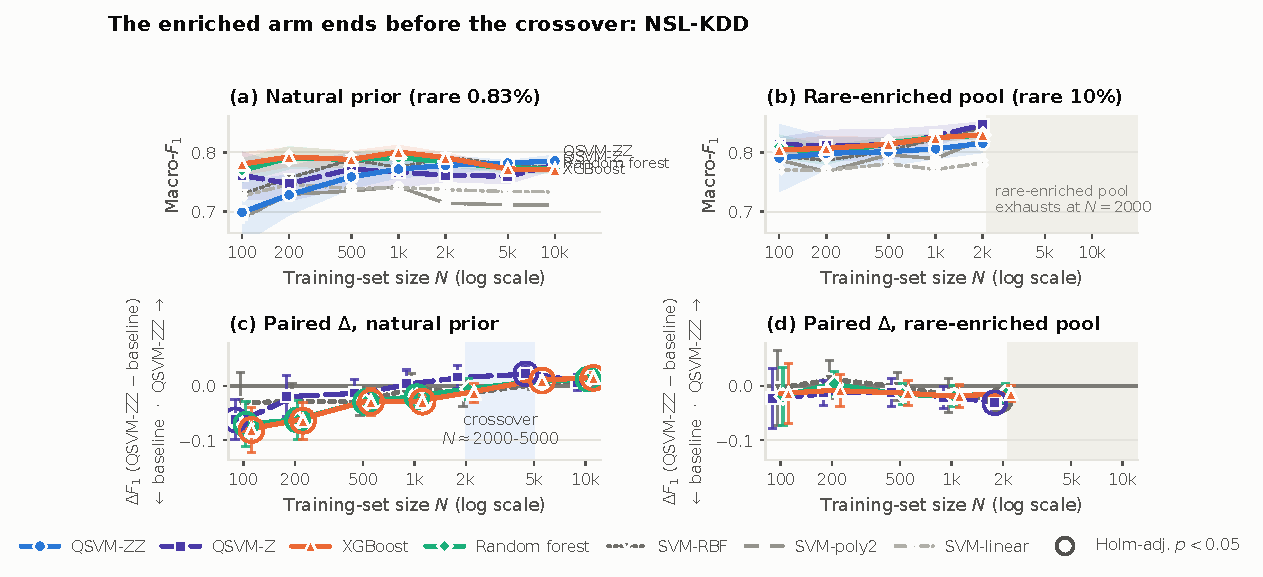
\includegraphics[width=\textwidth]{figs_revision/fig9_learning_curve_nslkdd.pdf}
  \caption{%
    \textbf{Under the natural prior the ordering reverses between $N=2000$ and
    $N=5000$; the rare-enriched arm ends before that interval.} (a,~b) Mean
    macro-$F_1$ over ten runs on the full KDDTest+ set with $95\%$ bands;
    (c,~d) paired differences against each baseline, circled where the
    Holm-adjusted $p<0.05$. The reversal against the tree ensembles and the
    linear and polynomial kernels lies in the band in (c); against SVM-RBF the
    sign change is $+0.0008$ and never significant. The enriched pool (b,~d)
    cannot be sampled past $N=2000$ without runs sharing rare samples, so it
    stops one step before the reversal; within the shared range the tree
    ensembles lead under both priors. Whether enrichment removes the reversal is
    therefore untested, not shown (Sec.~\ref{sec:res-c4}).}
  \label{fig:learning-curve}
\end{figure*}

\input{tables/ref_arm}
\begin{revbody}



The submitted version claimed an advantage in the low-data regime from a sweep
that stopped at $N=1000$. Extending it to $N=10^4$ under the natural class prior
reverses the claim and, in doing so, produces the paper's main new finding
(Fig.~\ref{fig:learning-curve}).

All seven models share the four-component front-end of
Sec.~\ref{sec:framework}, so the ranking below is a ranking of learners on
that embedding. At $N=100$ the ranking is XGBoost $0.7802$, random forest $0.7695$,
QSVM-\Zmap{} $0.7613$, SVM-RBF $0.7296$, linear $0.7261$, \QSVM{} $0.6989$: the
quantum kernel is next to last, and the gap to XGBoost, $-0.0812$, is the
largest in the sweep. At $N=10^4$ the ranking is \QSVM{} $0.7855$, QSVM-\Zmap{}
$0.7787$, SVM-RBF $0.7740$, random forest $0.7728$, XGBoost $0.7706$: the
quantum kernel is first among them. The paired difference against XGBoost passes through
zero between $N=2000$ and $N=5000$ ($-0.0129 \rightarrow +0.0100$), and is
corrected-significant at both $N=5000$ ($p_{\text{Holm}}=0.027$, $d_z=1.22$) and
$N=10^4$ ($+0.0149$, $p_{\text{Holm}}=0.0078$, $d_z=1.07$).

Four qualifications keep this from being read as more than it is.

First, the reversal is not an artefact of re-tuning.
Table~\ref{tab:crossover-arms} repeats the sweep with hyper-parameters frozen at
their C2 values instead of re-tuned at each $N$; all six baseline--arm
combinations change sign in the same interval, $2000\rightarrow5000$. A
re-tuning artefact would not survive freezing the tuning.

Second, the reversal is not uniform across baselines. Against SVM-RBF the
difference does turn positive, but no cell in the sweep reaches
corrected significance; the quantum kernel never demonstrably beats an RBF
kernel at any size we tested. Significance is reached against XGBoost at
$N\geq5000$, against the random forest only at $N=10^4$, and against the linear
and poly-2 kernels from $N=1000$ and $N=2000$ respectively.

Third, whether the reversal is a property of the natural prior cannot be
decided by this design, and an earlier draft of this paper claimed that it was.
Repeating the sweep with rare attacks enriched twelvefold to $10\%$, the
sampling the submitted protocol used, leaves $26$ of $30$ comparisons
inconclusive and shows no crossover in its range; but that range ends at
$N=2000$, because at $N=5000$ the ten runs would share $59\%$ of their rare
samples and independence between runs would be lost, and the crossover under
the natural prior occurs between $N=2000$ and $N=5000$, one step beyond it.
Within the range the two regimes share, the tree ensembles lead under both
priors: against XGBoost the paired difference is negative at all five sizes
under both, against the random forest and SVM-RBF at five of five under the
natural prior and four of five under enrichment, and the sign agrees in $22$ of
the $30$ shared cells; the enriched arm reaches a verdict in $4$ of its $30$
cells against $12$ of $30$ for the natural arm on the same sizes, most of the
difference being classical-favourable cells at $N\leq1000$ that enrichment
leaves inconclusive. The enriched arm therefore ends before the phenomenon begins, and
what the comparison establishes is that enrichment is untested against the
crossover, not that it removes it. What does follow for the submitted protocol
is narrower: a sweep confined to $N\leq2000$, under either prior, could not have
seen the regime in which the kernel does best.

Fourth, the reversal is a statement about the shared embedding, not about the
dataset. Table~\ref{tab:ref-arm} adds a reference arm outside the paired
protocol: XGBoost and the random forest trained on the same nested subsets and
seeds but on all $122$ one-hot features, scored on the same full KDDTest$^+$.
Full-feature XGBoost also declines with $N$ on this split, from
$\refArmXgbPeak$ at $N=\refArmXgbPeakN$ to $\refArmXgbTenK$ at $N=10^4$, and at
$N=5000$ and $N=10^4$ the paired difference against \QSVM{} is
$\refArmDeltaXgbFiveK$ and $\refArmDeltaXgbTenK$: parity, not a crossover.
Against the full-feature random forest the quantum kernel does lead at
$N=10^4$ ($\refArmDeltaRfTenK$). With the entire $125{,}973$-record partition,
full-feature XGBoost reaches $0.804$ (Sec.~\ref{sec:setup}), above the best
score of any four-qubit model in this paper. The practical reading is
therefore narrower than the ranking suggests: a four-qubit kernel matches, but
does not beat, a tree ensemble given the raw record.

\end{revbody}

\subsection{Rare attacks}
\label{sec:res-rare}
\revnote{new}{New subsection. The submitted version claimed ``+6.7 points on rare attacks, d=+0.68'' but the released code computed no rare-class metric (R4-5). That claim is withdrawn.}
\begin{revbody}

Because R2L and U2R are the classes an operator cares about, we report them
separately rather than only inside the macro average. At $N=10^4$ under the
natural prior the rare-class $F_1$ is SVM-RBF $0.585$, \QSVM{} $0.507$,
QSVM-\Zmap{} $0.421$, XGBoost $0.334$, random forest $0.331$, poly-2 $0.109$,
linear $0.089$.

Two things follow. The quantum kernel is far better on rare attacks than either
tree ensemble, which is not visible in the macro average and is worth knowing.
But SVM-RBF is better still, by $0.078$, so the honest statement is that an RBF
kernel is the strongest rare-attack detector in this study. The submitted
version reported a $+6.7$-point rare-attack gain with $d=+0.68$; no rare-class
metric was computed by the code that produced it, and we withdraw the number.
\end{revbody}

\subsection{Transfer to UNSW-NB15}
\label{sec:res-unsw}
\revnote{new}{New subsection. The submitted version mentioned UNSW-NB15 in one sentence of the limitations; AE-3 and R1-2 asked for a second dataset in full.}
\input{figs_revision/fig_unsw_transfer}
\begin{revbody}


The selection rule is applied to UNSW-NB15 without changing a threshold or a
constant (Fig.~\ref{fig:c1-selection}(b)). It returns $n^\ast=6$, at $V=0.9044$,
$\mathrm{KTA}=0.1986$ and $60$ two-qubit gates. Re-running it on ten
independent subsets returns $n^\ast=6$ in $10/10$ at tolerance
$\varepsilon\in\{0.02,0.05\}$ and $7/10$ at $\varepsilon=0.1$. That the rule
returns a different width on a different dataset is the point: it is a rule with
inputs, not a constant dressed as one.

The sample-complexity result does not transfer (Fig.~\ref{fig:unsw-transfer}). At
$N=10^4$, \QSVM{} is favourable against SVM-RBF ($+0.0401$,
$p_{\text{Holm}}=0.0059$) and against its own entanglement-free control
($+0.0449$, $p_{\text{Holm}}=0.0020$), but XGBoost stays ahead at every size
tested ($-0.0204$ at $N=10^4$, classical-favourable), and no crossover against
either tree ensemble occurs anywhere in the sweep. A finding that reproduces on
one dataset and not the other is reported as exactly that.
\end{revbody}

\subsection{Where the kernel breaks, and why}
\label{sec:res-width}
\revnote{new}{New subsection. Answers R3-4 (``very few qubits''): at 8 qubits all 48 comparisons favour the classical side, with the Gram-matrix mechanism measured.}
% Sinh boi runners/make_paper1_figures.py; caption doi chieu bang
% runners/audit_figures.py. File rieng cho tung hinh de \input DUNG CHO
% trong than bai -- float cua LaTeX chi troi VE SAU, khai bao het o cuoi
% tai lieu thi ca 9 hinh don xuong cuoi va tran vao danh muc tai lieu.

\begin{figure*}[t]
  \centering
  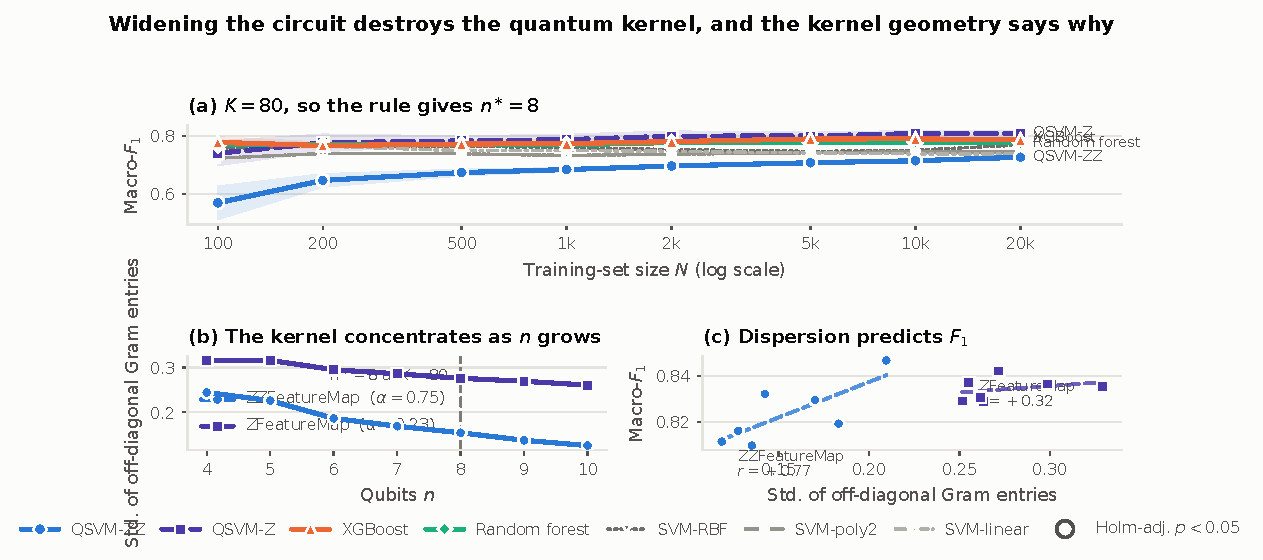
\includegraphics[width=\textwidth]{figs_revision/fig12_width_concentration.pdf}
  \caption{%
    \textbf{Widening the circuit destroys the quantum kernel, and the kernel
    geometry says why.} (a) The sample-complexity sweep re-run at $K=80$, where
    the rule returns $n^{\ast}=8$: all $48$ paired comparisons are
    classical-favourable. (b) Off-diagonal Gram dispersion against width, fitted
    as $n^{-\alpha}$ at $K=80$; the \ZZ{} map concentrates $3.3$ times as fast
    as the \Zmap{} map here ($\alpha=0.75$ against $0.23$), against the factor
    of $2.02$ at $K=20$ that phase-term counting predicts (Sec.~\ref{sec:res-width}).
    (c) Across widths the dispersion correlates with macro-$F_1$ at $r=+0.77$
    for \ZZ{} (95\% CI $[+0.04,+0.96]$) and $r=+0.32$ for \Zmap{}
    ($[-0.57,+0.87]$); the contrast between the two is not resolved at seven
    widths ($z=0.97$, $p=0.33$).}
  \label{fig:width}
\end{figure*}

\begin{revbody}


Sec.~\ref{sec:res-c1} showed that a larger feature budget forces a wider
circuit. Paying that price is the sharpest test of whether the quantum kernel
has headroom, and it fails it (Fig.~\ref{fig:width}).

Re-running the entire sample-complexity sweep at $K=80$, where the rule returns
$n^\ast=8$, produces $48$ paired comparisons (six baselines across eight
training-set sizes), and every one of them is classical-favourable. The
entanglement ablation reverses sign as well: at eight qubits \QSVM{} falls
\emph{below} its entanglement-free control at every size, by $0.082$ to $0.171$
macro-$F_1$. Widening the circuit does not extend the advantage; it removes it.

The mechanism is measurable in the Gram matrix rather than inferred. Writing
$s(n)$ for the standard deviation of the off-diagonal entries and fitting
$s(n)\propto n^{-\alpha}$ over $n=4,\dots,10$, we obtain $\alpha_{\ZZ}=0.590$
against $\alpha_{\Zmap}=0.292$ at $K=20$, a ratio of $2.02$. That ratio is
what the circuit structure predicts: the \ZZ{} map contributes
$\binom{n}{2}$ pairwise phase terms where the \Zmap{} map contributes $n$
single-qubit terms, so the former's phase content grows quadratically and the
latter's linearly. The prediction holds at $K=20$ and not at $K=80$, the budget
at which the collapse occurs: there the fitted exponents are $0.75$ against
$0.23$, a ratio of $3.32$ (Fig.~\ref{fig:width}b), and over the same range the
\ZZ{} kernel loses $49\%$ of its off-diagonal dispersion against $18\%$ for the
\Zmap{} kernel. The counting argument therefore predicts the ordering of the
two decay rates everywhere and their ratio only where the kernel does not
collapse; Sec.~\ref{sec:limitations} returns to this.

The concentration is not merely present; it tracks the end-task result. Across
$n=4,\dots,10$ the correlation between off-diagonal dispersion and macro-$F_1$
is $r=+0.77$ for the \ZZ{} kernel (95\% CI $[+0.04,+0.96]$, $p=0.04$ on seven
widths) and $r=+0.32$ for the \Zmap{} kernel ($[-0.57,+0.87]$, $p=0.48$), which
barely concentrates. The first correlation is resolved, barely; the contrast
between the two is not: a test of the difference between the two correlations
gives $z=0.97$, $p=0.33$, so the data do not establish that the relation is
specific to the concentrating map, and we do not claim that they do. As the Gram
matrix flattens, accuracy follows it down.
This is the exponential-concentration phenomenon of \cite{thanasilp2024} in a
concrete applied setting, and it is why we present a bounded operating window
rather than a method that scales.

An independent measurement supports the boundary and sharpens its
interpretation. Cirillo \emph{et al.} \cite{qmi2026}, sweeping qubit count on
the same corpus under backend-derived noise, locate good performance in a
$20$--$35$ two-qubit-gate band with degradation beyond roughly $60$ gates. Our
operating point of $24$ gates sits inside that band and our collapse at $112$
gates lies beyond their threshold, so the two studies agree on where the
usable window ends. They differ on why: that study attributes the degradation
to two-qubit gate error accumulating on hardware, whereas the results above are
obtained under exact, noiseless simulation, in which no gate error exists. The
window therefore does not widen with better hardware. It is set by the kernel.
\end{revbody}


% =====================================================================
\section{Regime Map: When to Use \QSVM{}}
\label{sec:regimemap}
% =====================================================================
%  VI. Regime Map
%
%  Muc nay la cho "doi khung": tu "chung toi co loi the" sang "day la ranh
%  gioi". So 21/21/68 phai xuat hien nguyen ven, khong duoc chi ke 21 thang.
%  Nguon: results/nslkdd/regime_map_rows.csv, doi chieu ca 110 dong bang
%  runners/audit_c4.py muc E.
% =====================================================================



% Sinh boi runners/make_paper1_figures.py; caption doi chieu bang
% runners/audit_figures.py. File rieng cho tung hinh de \input DUNG CHO
% trong than bai -- float cua LaTeX chi troi VE SAU, khai bao het o cuoi
% tai lieu thi ca 9 hinh don xuong cuoi va tran vao danh muc tai lieu.

\begin{figure*}[t]
  \centering
  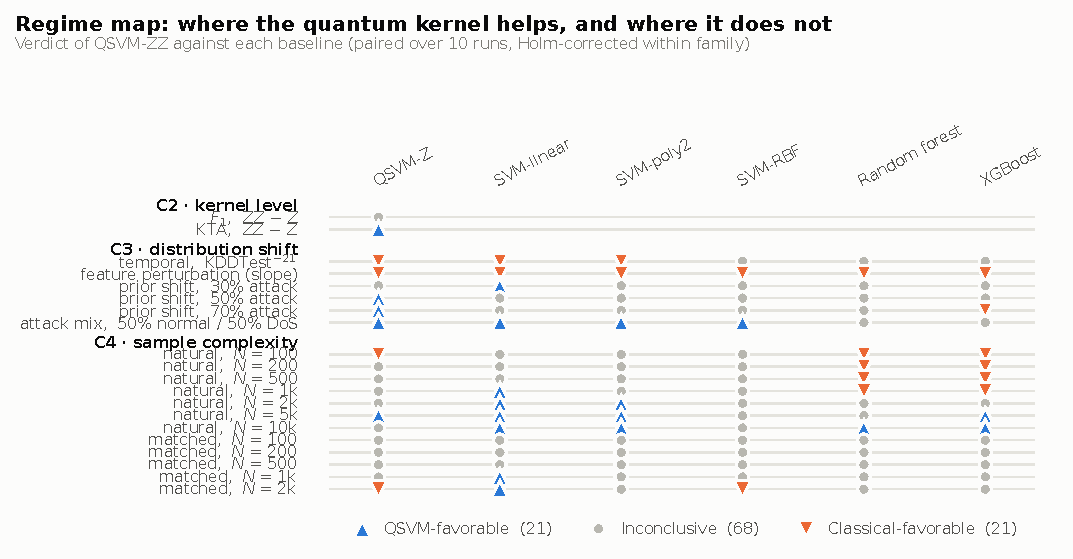
\includegraphics[width=\textwidth]{figs_revision/fig10_regime_map.pdf}
  \caption{%
    \textbf{Regime map: 110 controlled comparisons of \QSVM{} against six
    baselines.} Each cell is one paired comparison over ten runs, Holm-corrected
    within its baseline family (families of one to three; the $20$ cells
    against QSVM-\Zmap{} are uncorrected). Verdicts are encoded by both colour
    and glyph so the figure survives greyscale printing. The distribution is the
    result: $21$ favourable, $21$ classical-favourable, $68$ inconclusive within
    families; $17$, $15$ and $78$ under one Benjamini--Hochberg correction over
    all $110$ cells; and under Holm over all $110$ no cell survives. The seven
    C4-natural rows ($42$ cells) are the single-protocol block of
    Sec.~\ref{sec:regimemap}; the C2 and C3 rows are scored on a $300$- or
    $1000$-record test set. A single aggregate number would hide exactly the
    structure this paper is about.}
  \label{fig:regime-map}
\end{figure*}


Collecting every controlled comparison in one place gives the map in
Fig.~\ref{fig:regime-map}: $110$ cells, each a paired comparison between
\QSVM{} and one baseline under one condition, each carrying a Holm-corrected
verdict. Twenty-one favour the quantum kernel, twenty-one favour a classical
baseline, and sixty-eight are inconclusive. Two qualifications attach to that
count. The cells are corrected within families of one to three
(Sec.~\ref{sec:stats}); under a single Benjamini--Hochberg correction over all
$110$ cells the tally is $17$, $15$ and $78$, every cell that changes moving to
inconclusive and none changing side, and under Holm over all $110$ no cell
survives. And the cells come from two protocols that Sec.~\ref{sec:setup} says
are not interchangeable: $42$ cells from the natural prior on the full
KDDTest$^+$ partition (11 favourable, 9 unfavourable, 22 inconclusive) and $68$
from the rare-enriched pool (10, 12, 46), of which $30$ are scored on the full
partition and $38$ on a $300$-record or re-mixed $1000$-record test set. A
difference estimated on $300$ records and one estimated on $22{,}544$ do not
carry the same weight, and the reader who wants a single-protocol map should
read the natural-prior block on its own.

The balance of the first two numbers is the honest summary of this study. A
practitioner reading only the count would conclude that the quantum kernel is
neither better nor worse on average, and that conclusion would be correct and
useless. The map is worth more than its margin because the verdicts are not
distributed at random across conditions.

\subsection{Where it is worth the cost}
\revnote{rewrite}{The submitted forest plot had 9 rows; now 110 cells, each with $\Delta$, CI, $p$ and $d_z$ (R2-4).}
\begin{revbody}

Three conditions produce a favourable verdict, and they share a structure.

\emph{Enough data, natural prior.} At $N\geq5000$ under the natural class prior,
\QSVM{} is favourable against XGBoost and, at $N=10^{4}$, against the random
forest; it is favourable against the linear and poly-2 kernels from $N=1000$ and
$N=2000$. Below $N=2000$ the verdicts run the other way. The regime is bounded
on both sides: below it the kernel has too little data, and
Sec.~\ref{sec:res-width} shows that a wider circuit does not extend it upward.
It is also bounded from above by a model outside the paired protocol: every
favourable verdict here is against a baseline given the same four components,
and against XGBoost given all $122$ features the kernel reaches parity at
$N\geq5000$ (Table~\ref{tab:ref-arm}), while XGBoost on the full training
partition scores $0.804$, above any four-qubit model in this paper
(Sec.~\ref{sec:setup}). The regime is where the kernel is worth its cost
relative to a classical learner on the same embedding, not relative to the best
classical score available on the record.

\emph{Balanced binary composition.} On a $50/50$ Normal--DoS mixture the quantum
kernel is favourable against all four kernel baselines, with effect sizes up to
$3.02$. This is a C3 cell: models trained on the rare-enriched $N=1000$ pool
and scored on a re-mixed $1000$-record test set, so it lies outside the
natural-prior block and is not visible in the single-protocol reading. This is the condition under which quantum-kernel IDS results are most
often reported in the literature, and our numbers reproduce that impression;
which is part of why we report the other conditions too.

\emph{Rare-attack detection relative to tree ensembles.} At $N=10^{4}$ the
rare-class $F_{1}$ of \QSVM{} is $0.507$ against $0.334$ for XGBoost and $0.331$
for the random forest. If the deployment objective is rare-attack recall rather
than macro-averaged accuracy, the ranking changes substantially, though
SVM-RBF, at $0.585$, remains ahead of both.
\end{revbody}

\subsection{Where it is not}
\revnote{rewrite}{R2-4 observed that favourable regimes received full statistics and unfavourable ones only qualitative remarks; both sides now receive the same treatment.}
\begin{revbody}

\emph{Small training sets.} At $N\leq500$ the quantum kernel loses to both tree
ensembles at every size, by up to $0.081$ macro-$F_{1}$. No configuration we
tested recovers this.

\emph{Feature perturbation.} Six of six comparisons are classical-favourable
with effect sizes beyond $2.8$. The quantum kernel is the most perturbation-%
sensitive model in the study, which matters for a security application where
adversarial feature manipulation is the norm rather than the exception. Like
the balanced-composition result above, this is a C3 cell on the rare-enriched
pool and a $1000$-record test set, outside the natural-prior block; the two
clearest effect sizes in the map both come from that protocol.

\emph{Strong prior shift.} At a $70\%$ attack rate the comparison against
XGBoost is classical-favourable, and \QSVM{} degrades across the shift by
$0.032$ against $0.021$ for XGBoost. The submitted version presented this regime
as its strongest evidence; against strong tabular baselines it is evidence in
the opposite direction.

\emph{Wide circuits.} At $K=80$ and $n^{\ast}=8$, all $48$ comparisons are
classical-favourable. This is the sharpest boundary we found and the least
expected: it says the operating window is closed from above by the physics of
the feature map rather than by engineering limits that better hardware would
lift.

\emph{Any comparison against SVM-RBF on sample size.} Across the whole sweep, no
cell reaches corrected significance in the quantum kernel's favour. An RBF
kernel is the baseline this method does not clear.
\end{revbody}

\subsection{Reading the map}
\revnote{new}{New subsection, absorbing the ``decision rule'' of the submitted version.}
\begin{revbody}

Two properties of the map should govern how it is generalised.

First, the inconclusive cells are the majority, and they are informative. With
ten runs and Holm correction the smallest difference that reaches a verdict
anywhere in the map is $0.010$ macro-$F_1$, while differences as large as
$0.031$ remain inconclusive when their run-to-run spread is wide; the median
inconclusive cell sits at $0.014$. Most of the differences in this study are of
that order. A study reporting sharper verdicts on the same data with fewer
repetitions and no multiplicity control is not seeing more; it is resolving
less.

Second, the favourable regime is bounded on every axis we varied, and the
bounds are not far apart: $N \gtrsim 5000$ but not at a width beyond four to six
qubits, on NSL-KDD but not on UNSW-NB15 for the sample-size effect, and under
the natural prior, with the enriched prior untested at the sizes where the
regime lies. A method whose advantage is confined to a
box this small is not yet a practical instrument, and we do not present it as
one. What it is, on this evidence, is a phenomenon with a measurable boundary
and the boundary, being predicted by the circuit's phase-term count, is the
part most likely to hold beyond these two datasets.
\end{revbody}


% =====================================================================
% =====================================================================
%  Muc VII viet lai -- TETC-2026-05-0252
%
%  Ban da nop hua ba thu la "ongoing work" hoac "deferred": (a) do tac dong
%  cua be rong mach, (b) so voi baseline khong phai SVM, (c) dataset thu hai.
%  Ca ba nay bay gio deu co so do, nen muc han che khong con la loi hua ma la
%  bao cao ket qua kem ranh gioi ro rang.
%
%  Cho DUY NHAT van con la loi hua: thuc thi tren QPU that. Phai ghi that ro
%  da lam gi va CHUA lam gi -- neu de mo ho thi reviewer se doc "NISQ-aware"
%  thanh mot khang dinh ve phan cung ma bai khong do duoc.
% =====================================================================

\section{Limitations and Threats to Validity}
\label{sec:limitations}

\subsection{Hardware noise: what was and was not measured}
\revnote{rewrite}{The submitted version covered finite-shot error only. A backend-derived noise model is added (AE-6, R1-6, R3-4), with a statement of what is not measured.}
\begin{revbody}

The submitted version reported only finite-shot sampling error and deferred
coherent noise to a companion study. Reviewers correctly objected that shot
noise alone cannot support a NISQ-feasibility claim. We therefore state the
scope precisely.

\emph{What we measure.} The C2 pipeline is re-run under a noise model derived
from the published calibration data of a real superconducting backend
(\texttt{FakeManilaV2}) \cite{ref27} via \texttt{NoiseModel.from\_backend}, which
carries gate errors, readout errors, and gate-duration-dependent thermal
relaxation.
Circuits are transpiled onto that backend's coupling map and basis gate set,
giving a depth of $59$ and $44$ two-qubit gates for the $n=4$, $r=2$ map.
Under this model the entanglement conclusion is unchanged: the alignment gap
between QSVM-ZZ and QSVM-Z survives, while the macro-$F_1$ difference remains
within its confidence interval. This noisy re-run covers one of the ten runs
and the $300$-record test split (Table~\ref{tab:protocol}); it establishes
that the noise model does not move the operating point, not a noisy confidence
interval, which would require the remaining nine runs at the same $512$ shots
per kernel entry.

\emph{What we do not measure.} The circuits were not executed on a quantum
processor. Two effects are therefore outside our evidence: drift of calibration
parameters between the snapshot and execution time, and idle-time decoherence
beyond what gate durations already attribute. Our released code contains the
execution path for a real backend, and the comparison it would produce
(exact statevector $\rightarrow$ backend-derived noise $\rightarrow$ hardware)
is specified, but we report no hardware numbers and make no claim about them.
Readers should read ``NISQ-aware'' as a statement about \emph{circuit budget}
(qubit count, depth, and two-qubit gate count chosen under an explicit cost
model, in the sense of \cite{ref8}) and not as a claim of hardware validation.
\end{revbody}

\subsection{Embedding size: now measured, and the news is not good for width}
\revnote{fix}{The submitted version left this as an ``open question''; it is now measured, and the result is unfavourable to wider circuits.}
\begin{revbody}

The submitted version listed the effect of moving along the frontier as an open
question. We have since measured it, and the answer constrains the method more
sharply than we expected.

Increasing the feature budget $K$ does buy accuracy for a classical proxy, but
it is not free: retaining $85\%$ of the variance at $K=80$ requires $n^\ast=8$
qubits rather than the $n^\ast=4$ that $K=20$ admits, raising the two-qubit gate
count from $24$ to $112$. Re-running the full sample-complexity sweep at that
operating point removes the quantum kernel's advantage entirely: across eight
training-set sizes and six baselines, all $48$ paired comparisons favour the
classical model, and the entanglement ablation reverses sign, with QSVM-ZZ now
\emph{below} its entanglement-free control.

The mechanism is measurable rather than conjectural. The dispersion of the
off-diagonal Gram entries decays with width as $n^{-\alpha}$, and the fitted
exponent for the ZZ map is close to twice that of the Z map at $K=20$
($0.59$ vs.\ $0.29$), consistent with the $\binom{n}{2}$ pairwise phase terms of
the former growing quadratically where the latter's grow linearly. Across
$n=4$ to $10$ the macro-$F_1$ of the ZZ kernel tracks this dispersion
($r=+0.77$, 95\% CI $[+0.04,+0.96]$), whereas the Z kernel, which barely
concentrates, shows no resolved dependence ($r=+0.32$, $[-0.57,+0.87]$). This is
the concentration phenomenon of \cite{thanasilp2024} appearing directly in our
setting.

Three caveats. The exponent ratio is $2.02$ at $K=20$, where the kernel does not
collapse, and $3.32$ at $K=80$, where it does, so the term-counting argument
predicts the ordering of the two rates and, at the collapse, not their ratio;
the abstract and Sec.~\ref{sec:intro} state both values. The $F_1$--dispersion
relation is measured on seven widths at a single training-set size, and the
contrast between the two kernels' correlations is not resolvable at seven
points ($z=0.97$, $p=0.33$); we present the relation as an empirical regularity
of the \ZZ{} map, not a law, and make no claim that it is specific to the
concentrating map. A test of either would need more widths and more than one
training-set size.
\end{revbody}

\subsection{Classical-baseline strength}
\revnote{rewrite}{RF and XGBoost added; CatBoost, TabNet and FT-Transformer deliberately not added, with the reason stated (R1-5).}
\begin{revbody}

The submitted version compared only against SVM variants. We have added a
random forest and XGBoost under the identical protocol, and they change the
headline: on the main benchmark XGBoost attains the highest mean macro-$F_1$
($0.8503$) ahead of QSVM-ZZ ($0.8469$), with overlapping intervals. We report
this as an ordering of point estimates, not a significant separation.

We did not add CatBoost or deep tabular models such as TabNet and
FT-Transformer. CatBoost would supply a second gradient-boosting representative
without changing the comparison structure; the deep tabular family would require
its own tuning-budget protocol to be compared fairly, which would enlarge the
study from a controlled quantum-kernel benchmark into a survey of tabular
architectures. We therefore do not claim coverage of all strong tabular methods,
and any practical reading of our results should be qualified accordingly.
\end{revbody}

\subsection{Dataset breadth and protocol}
\revnote{rewrite}{UNSW-NB15 added, with duplication statistics for both corpora.}
\begin{revbody}

The submitted version rested almost entirely on NSL-KDD. We have added
UNSW-NB15 under the same protocol, which is what allows us to separate findings
that transfer from findings that do not: the dimension-selection rule and the
entanglement ablation transfer, while the sample-complexity crossover and the
rare-class behaviour do not.

Two properties of the data limit what either dataset can show. NSL-KDD is an
aging benchmark in which $610$ test rows are identical to a training row in both
features and label ($617$ match on features alone). UNSW-NB15 is far more heavily
duplicated: $47.3\%$ of training rows are internal repeats, and $25.0\%$ of test
rows have an exact duplicate in the training partition, which
inflates absolute scores. Our claims are paired differences between models
evaluated on the same rows, which removes the duplication from the level but
not necessarily from the comparison: a tree ensemble reproduces an exact
training row by construction, a fidelity-kernel SVM does so only through its
support vectors and regulariser, and on the quarter of the UNSW-NB15 test set
that duplicates a training row a paired difference may therefore measure
memorisation rather than generalisation. We have not re-scored the paired
differences on the de-duplicated test subsets, because the sweep's per-row
predictions were not retained, and we list that re-scoring as the one cheap
check this study owes: until it is done, the UNSW-NB15 verdicts, and to a
smaller degree the NSL-KDD ones, carry this threat, and the absolute numbers
are not comparable to studies that de-duplicate.

Finally, the feature budget $K=20$ is inherited from the submitted protocol and
held fixed so that the revised results remain comparable to it.
Fig.~\ref{fig:ksweep} shows it is not the accuracy optimum; it is the value at
which the selection rule returns a four-qubit circuit.
\end{revbody}
            % Sec VII, da co \section ben trong

% =====================================================================
\section{Conclusion and Future Work}
\label{sec:conclusion}
% =====================================================================
%  VIII. Conclusion
%
%  Khong duoc ket bang "ket qua hua hen". Ket bang cai ta do duoc va cai
%  ta khong do duoc. Cau cuoi cung phai la mot cau kiem chung duoc.
% =====================================================================

\revnote{rewrite}{Rewritten: the advantage claim is replaced by the boundary the regime map draws (AE-1, R1-4, R3-2).}
\begin{revbody}
We set out to locate, rather than to demonstrate, the value of a NISQ-feasible
quantum kernel for network intrusion detection. Varying one factor at a time
over $110$ controlled comparisons, we find $21$ verdicts favouring the quantum
kernel, $21$ favouring a classical baseline, and $68$ inconclusive when each
is corrected within its baseline family; $17$, $15$ and $78$ under one
Benjamini--Hochberg correction over the map; and no surviving verdict at all
under Holm over all $110$ cells. Inside that balance there is a structure that
a single-operating-point benchmark cannot see, and it is stated below with the
protocol each part of it comes from.

The structure has three parts. The ordering between \QSVM{} and the tree
ensembles and the linear and polynomial kernels reverses between $N=2000$ and
$N=5000$ under the natural class prior, in both tuning arms, on a shared
four-component embedding; it does not demonstrably reverse against SVM-RBF at
any size tested, it becomes parity rather than a lead against XGBoost on the raw
$122$ features, and whether rare-attack enrichment removes it is not decided by
this design, whose enriched arm ends before the reversal begins. A
lexicographic selection rule that charges for two-qubit gates returns
$n^{\ast}=4$ on NSL-KDD and $n^{\ast}=6$ on UNSW-NB15 without any change of
threshold, so the embedding dimension is a property of the dataset rather than a
constant to be inherited. And the operating window is closed from above: at
$K=80$, where the rule requires eight qubits, every one of $48$ comparisons
favours the classical model, with off-diagonal Gram dispersion decaying faster
for the \ZZ{} map than for its entanglement-free control, by the factor of two
that phase-term counting predicts at $K=20$ and by $3.3$ at $K=80$, and tracking
macro-$F_1$ at $r=+0.77$ over seven widths (95\% CI $[+0.04,+0.96]$).

That last result is the one we would most like others to test. It ties a
structural property of the circuit ($\binom{n}{2}$ pairwise phase terms
against $n$ single-qubit ones) to a decay exponent we can measure and to an
end-task metric that follows it down. If it holds on other corpora and other
maps, then the practical question for quantum kernels on tabular data is not how
to make them more expressive but how to keep them from concentrating, and the
useful width is bounded well below where hardware limits bite.

We are equally clear about what this study does not establish. The circuits were
not executed on a quantum processor, and ``NISQ-aware'' here means a circuit
budget chosen under an explicit cost model, not hardware validation. The
comparison covers two datasets, two tree ensembles and three kernel baselines,
not the deep tabular architectures. The favourable regime is narrow on every
axis we varied. And five claims from the earlier version of this work do not
survive the revised protocol; they are withdrawn in Sec.~\ref{sec:intro} and
corrected in Sec.~\ref{sec:erratum}.

Three directions follow directly. Executing the same kernels on hardware would
close the one gap our simulations cannot: the released code contains the
execution path and the three-tier comparison it would produce is already
specified. Testing the dispersion--accuracy relationship on projected quantum
kernels, which concentrate differently, would show whether the boundary we
measured is a property of fidelity kernels specifically or of the approach.
And since the crossover reproduces on one dataset and not the other, the
mechanism behind it, why more data helps this kernel more than it helps a
tree ensemble and only under a skewed prior, remains open. Our full
implementation, protocol files, intermediate artifacts and two independent audit
scripts are released so that each of these can be started from where we stopped.
\end{revbody}


% =====================================================================
%  Phu luc: chung minh Lemma 1. Ban da nop hua "Appendix A" nhung IEEEtran
%  can \appendices tuong minh -- lenh do nam trong file duoi.
% =====================================================================
\input{sections/09_appendix}

% =====================================================================
\section*{Acknowledgment}
This work was supported by The University of Danang - University of Science
and Technology, project T2026-02-10TN. The authors thank Danang Architecture
University for computing resources, and the maintainers of Qiskit and
scikit-learn.
\begin{revbody}
The authors used Anthropic's Claude (Opus~5) as an assistant during the
preparation of this revision. Its use covered three areas: drafting and editing
prose throughout the manuscript and the response letter; writing the analysis,
audit and experiment-orchestration scripts released with the artifact; and
proposing measurements reported in Secs.~IV and~V, among them the symmetric
tuning arms, the protocol-by-contribution table, the full-feature reference arm
(Table~IV) and the audit scripts. All experimental results were produced by
executing the released code, and every number reported here was checked
against the run records by the authors, who take full responsibility for the
content of this paper.
\end{revbody}

% =====================================================================
%  Danh muc tai lieu. TUNG co \clearpage o day lam chot chan chong hinh
%  xen vao giua cac muc tai lieu; da bo vi nguyen nhan goc (ca 9 hinh khai
%  bao o cuoi tai lieu) da sua, va chot chan do lam trong nua trang truoc
%  phan References.
% =====================================================================
% =====================================================================
\input{bibliography}           % 35 muc; xem ghi chu trong file

% 13/09/2026: tieu su 5 tac gia (TETC yeu cau trong ban revise; ban da nop co)
\input{sections/10_biographies}

\end{document}
